\documentclass[oneside,11pt]{book} 

\usepackage[utf8]{inputenc} \usepackage[T1]{fontenc} \usepackage{listings}
\usepackage{color}
\usepackage[svgnames]{xcolor}
\usepackage{textcomp}
\usepackage{graphicx}
\usepackage{subcaption}
\usepackage{float}
\usepackage{footnote}  \usepackage{newfloat}
\def\PsfigVersion{1.10}
\def\setDriver{\DvipsDriver} \ifx\undefined\psfig\else\endinput\fi


\let\LaTeXAtSign=\@
\let\@=\relax
\edef\psfigRestoreAt{\catcode`\@=\number\catcode`@\relax}
\catcode`\@=11\relax
\newwrite\@unused
\def\ps@typeout#1{{\let\protect\string\immediate\write\@unused{#1}}}

\def\DvipsDriver{
	\ps@typeout{psfig/tex \PsfigVersion -dvips}
\def\PsfigSpecials{\DvipsSpecials} 	\def\ps@dir{/}
\def\ps@predir{} }
\def\OzTeXDriver{
	\ps@typeout{psfig/tex \PsfigVersion -oztex}
	\def\PsfigSpecials{\OzTeXSpecials}
	\def\ps@dir{:}
	\def\ps@predir{:}
	\catcode`\^^J=5
}



\def\figurepath{./:}
\def\psfigurepath#1{\edef\figurepath{#1:}}

\def\DoPaths#1{\expandafter\EachPath#1\stoplist}
\def\leer{}
\def\EachPath#1:#2\stoplist{\ExistsFile{#1}{\SearchedFile}
  \ifx#2\leer
  \else
    \expandafter\EachPath#2\stoplist
  \fi}
\def\ps@dir{/}
\def\ExistsFile#1#2{\openin1=\ps@predir#1\ps@dir#2
   \ifeof1
       \closein1
\else
       \closein1
\ifx\ps@founddir\leer
\edef\ps@founddir{#1}
        \fi
   \fi}
\def\get@dir#1{\def\ps@founddir{}
  \def\SearchedFile{#1}
  \DoPaths\figurepath
}



\def\@nnil{\@nil}
\def\@empty{}
\def\@psdonoop#1\@@#2#3{}
\def\@psdo#1:=#2\do#3{\edef\@psdotmp{#2}\ifx\@psdotmp\@empty \else
    \expandafter\@psdoloop#2,\@nil,\@nil\@@#1{#3}\fi}
\def\@psdoloop#1,#2,#3\@@#4#5{\def#4{#1}\ifx #4\@nnil \else
       #5\def#4{#2}\ifx #4\@nnil \else#5\@ipsdoloop #3\@@#4{#5}\fi\fi}
\def\@ipsdoloop#1,#2\@@#3#4{\def#3{#1}\ifx #3\@nnil 
       \let\@nextwhile=\@psdonoop \else
      #4\relax\let\@nextwhile=\@ipsdoloop\fi\@nextwhile#2\@@#3{#4}}
\def\@tpsdo#1:=#2\do#3{\xdef\@psdotmp{#2}\ifx\@psdotmp\@empty \else
    \@tpsdoloop#2\@nil\@nil\@@#1{#3}\fi}
\def\@tpsdoloop#1#2\@@#3#4{\def#3{#1}\ifx #3\@nnil 
       \let\@nextwhile=\@psdonoop \else
      #4\relax\let\@nextwhile=\@tpsdoloop\fi\@nextwhile#2\@@#3{#4}}
\ifx\undefined\fbox
\newdimen\fboxrule
\newdimen\fboxsep
\newdimen\ps@tempdima
\newbox\ps@tempboxa
\fboxsep = 3pt
\fboxrule = .4pt
\long\def\fbox#1{\leavevmode\setbox\ps@tempboxa\hbox{#1}\ps@tempdima\fboxrule
    \advance\ps@tempdima \fboxsep \advance\ps@tempdima \dp\ps@tempboxa
   \hbox{\lower \ps@tempdima\hbox
  {\vbox{\hrule height \fboxrule
          \hbox{\vrule width \fboxrule \hskip\fboxsep
          \vbox{\vskip\fboxsep \box\ps@tempboxa\vskip\fboxsep}\hskip 
                 \fboxsep\vrule width \fboxrule}
                 \hrule height \fboxrule}}}}
\fi
\newread\ps@stream
\newif\ifnot@eof       \newif\if@noisy        \newif\if@atend        \newif\if@psfile       {\catcode`\%=12\global\gdef\epsf@start{\def\epsf@PS{PS}
\def\epsf@getbb#1{\openin\ps@stream=\ps@predir#1
\ifeof\ps@stream\ps@typeout{Error, File #1 not found}\else
{\not@eoftrue \chardef\other=12
    \def\do##1{\catcode`##1=\other}\dospecials \catcode`\ =10
    \loop
       \if@psfile
	  \read\ps@stream to \epsf@fileline
       \else{
	  \obeyspaces
          \read\ps@stream to \epsf@tmp\global\let\epsf@fileline\epsf@tmp}
       \fi
       \ifeof\ps@stream\not@eoffalse\else
\if@psfile\else
       \expandafter\epsf@test\epsf@fileline:. \\\fi
\expandafter\epsf@aux\epsf@fileline:. \\\fi
   \ifnot@eof\repeat
   }\closein\ps@stream\fi}\long\def\epsf@test#1#2#3:#4\\{\def\epsf@testit{#1#2}
			\ifx\epsf@testit\epsf@start\else
\ps@typeout{Warning! File does not start with `\epsf@start'.  It may not be a PostScript file.}
			\fi
			\@psfiletrue} {\catcode`\%=12\global\let\epsf@percent=\long\def\epsf@aux#1#2:#3\\{\ifx#1\epsf@percent
   \def\epsf@testit{#2}\ifx\epsf@testit\epsf@bblit
	\@atendfalse
        \epsf@atend #3 . \\\if@atend	
	   \if@verbose{
		\ps@typeout{psfig: found `(atend)'; continuing search}
	   }\fi
        \else
        \epsf@grab #3 . . . \\\not@eoffalse
        \global\no@bbfalse
        \fi
   \fi\fi}\def\epsf@grab #1 #2 #3 #4 #5\\{\global\def\epsf@llx{#1}\ifx\epsf@llx\empty
      \epsf@grab #2 #3 #4 #5 .\\\else
   \global\def\epsf@lly{#2}\global\def\epsf@urx{#3}\global\def\epsf@ury{#4}\fi}\def\epsf@atendlit{(atend)} 
\def\epsf@atend #1 #2 #3\\{\def\epsf@tmp{#1}\ifx\epsf@tmp\empty
      \epsf@atend #2 #3 .\\\else
   \ifx\epsf@tmp\epsf@atendlit\@atendtrue\fi\fi}




\chardef\psletter = 11 \chardef\other = 12

\newif \ifdebug \newif\ifc@mpute \c@mputetrue 

\let\then = \relax
\def\r@dian{pt }
\let\r@dians = \r@dian
\let\dimensionless@nit = \r@dian
\let\dimensionless@nits = \dimensionless@nit
\def\internal@nit{sp }
\let\internal@nits = \internal@nit
\newif\ifstillc@nverging
\def \Mess@ge #1{\ifdebug \then \message {#1} \fi}

{ \catcode `\@ = \psletter
	\gdef \nodimen {\expandafter \n@dimen \the \dimen}
	\gdef \term #1 #2 #3{\edef \t@ {\the #1}\edef \t@@ {\expandafter \n@dimen \the #2\r@dian}\t@rm {\t@} {\t@@} {#3}}
	\gdef \t@rm #1 #2 #3{{\count 0 = 0
		\dimen 0 = 1 \dimensionless@nit
		\dimen 2 = #2\relax
		\Mess@ge {Calculating term #1 of \nodimen 2}\loop
		\ifnum	\count 0 < #1
		\then	\advance \count 0 by 1
			\Mess@ge {Iteration \the \count 0 \space}\Multiply \dimen 0 by {\dimen 2}\Mess@ge {After multiplication, term = \nodimen 0}\Divide \dimen 0 by {\count 0}\Mess@ge {After division, term = \nodimen 0}\repeat
		\Mess@ge {Final value for term #1 of 
				\nodimen 2 \space is \nodimen 0}\xdef \Term {#3 = \nodimen 0 \r@dians}\aftergroup \Term
	       }}
	\catcode `\p = \other
	\catcode `\t = \other
	\gdef \n@dimen #1pt{#1} }

\def \Divide #1by #2{\divide #1 by #2} 

\def \Multiply #1by #2{{\count 0 = #1\relax
	\count 2 = #2\relax
	\count 4 = 65536
	\Mess@ge {Before scaling, count 0 = \the \count 0 \space and
			count 2 = \the \count 2}\ifnum	\count 0 > 32767 \then	\divide \count 0 by 4
		\divide \count 4 by 4
	\else	\ifnum	\count 0 < -32767
		\then	\divide \count 0 by 4
			\divide \count 4 by 4
		\else
		\fi
	\fi
	\ifnum	\count 2 > 32767 \then	\divide \count 2 by 4
		\divide \count 4 by 4
	\else	\ifnum	\count 2 < -32767
		\then	\divide \count 2 by 4
			\divide \count 4 by 4
		\else
		\fi
	\fi
	\multiply \count 0 by \count 2
	\divide \count 0 by \count 4
	\xdef \product {#1 = \the \count 0 \internal@nits}\aftergroup \product
       }}

\def\r@duce{\ifdim\dimen0 > 90\r@dian \then   \multiply\dimen0 by -1
		\advance\dimen0 by 180\r@dian
		\r@duce
	    \else \ifdim\dimen0 < -90\r@dian \then  \advance\dimen0 by 360\r@dian
		\r@duce
		\fi
	    \fi}

\def\Sine#1{{\dimen 0 = #1 \r@dian
	\r@duce
	\ifdim\dimen0 = -90\r@dian \then
	   \dimen4 = -1\r@dian
	   \c@mputefalse
	\fi
	\ifdim\dimen0 = 90\r@dian \then
	   \dimen4 = 1\r@dian
	   \c@mputefalse
	\fi
	\ifdim\dimen0 = 0\r@dian \then
	   \dimen4 = 0\r@dian
	   \c@mputefalse
	\fi
\ifc@mpute \then
\divide\dimen0 by 180
		\dimen0=3.141592654\dimen0
\dimen 2 = 3.1415926535897963\r@dian \divide\dimen 2 by 2 \Mess@ge {Sin: calculating Sin of \nodimen 0}\count 0 = 1 \dimen 2 = 1 \r@dian \dimen 4 = 0 \r@dian \loop
			\ifnum	\dimen 2 = 0 \then	\stillc@nvergingfalse 
			\else	\stillc@nvergingtrue
			\fi
			\ifstillc@nverging \then	\term {\count 0} {\dimen 0} {\dimen 2}\advance \count 0 by 2
				\count 2 = \count 0
				\divide \count 2 by 2
				\ifodd	\count 2 \then	\advance \dimen 4 by \dimen 2
				\else	\advance \dimen 4 by -\dimen 2
				\fi
		\repeat
	\fi		
			\xdef \sine {\nodimen 4}}}

\def\Cosine#1{\ifx\sine\UnDefined\edef\Savesine{\relax}\else
		             \edef\Savesine{\sine}\fi
	{\dimen0=#1\r@dian\advance\dimen0 by 90\r@dian
	 \Sine{\nodimen 0}
	 \xdef\cosine{\sine}
	 \xdef\sine{\Savesine}}}	      


\def\psdraft{
	\def\@psdraft{0}
}
\def\psfull{
	\def\@psdraft{100}
}

\psfull

\newif\if@scalefirst
\def\psscalefirst{\@scalefirsttrue}
\def\psrotatefirst{\@scalefirstfalse}
\psrotatefirst

\newif\if@draftbox
\def\psnodraftbox{
	\@draftboxfalse
}
\def\psdraftbox{
	\@draftboxtrue
}
\@draftboxtrue

\newif\if@prologfile
\newif\if@postlogfile
\def\pssilent{
	\@noisyfalse
}
\def\psnoisy{
	\@noisytrue
}
\psnoisy
\newif\if@bbllx
\newif\if@bblly
\newif\if@bburx
\newif\if@bbury
\newif\if@height
\newif\if@width
\newif\if@rheight
\newif\if@rwidth
\newif\if@angle
\newif\if@clip
\newif\if@verbose
\def\@p@@sclip#1{\@cliptrue}
\newif\if@decmpr
\def\@p@@sfigure#1{\def\@p@sfile{null}\def\@p@sbbfile{null}\@decmprfalse
\openin1=\ps@predir#1
   \ifeof1
	\closein1
\get@dir{#1}
	\ifx\ps@founddir\leer
\openin1=\ps@predir#1.bb
		\ifeof1
			\closein1
\get@dir{#1.bb}
			\ifx\ps@founddir\leer
\ps@typeout{Can't find #1 in \figurepath}
			\else
\@decmprtrue
				\def\@p@sfile{\ps@founddir\ps@dir#1}
				\def\@p@sbbfile{\ps@founddir\ps@dir#1.bb}
			\fi
		\else
			\closein1
\@decmprtrue
			\def\@p@sfile{#1}
			\def\@p@sbbfile{#1.bb}
		\fi
	\else
\def\@p@sfile{\ps@founddir\ps@dir#1}
		\def\@p@sbbfile{\ps@founddir\ps@dir#1}
	\fi
   \else
\closein1
	\def\@p@sfile{#1}
	\def\@p@sbbfile{#1}
   \fi
}
\def\@p@@sfile#1{\@p@@sfigure{#1}}
\def\@p@@sbbllx#1{
\@bbllxtrue
		\dimen100=#1
		\edef\@p@sbbllx{\number\dimen100}
}
\def\@p@@sbblly#1{
\@bbllytrue
		\dimen100=#1
		\edef\@p@sbblly{\number\dimen100}
}
\def\@p@@sbburx#1{
\@bburxtrue
		\dimen100=#1
		\edef\@p@sbburx{\number\dimen100}
}
\def\@p@@sbbury#1{
\@bburytrue
		\dimen100=#1
		\edef\@p@sbbury{\number\dimen100}
}
\def\@p@@sheight#1{
		\@heighttrue
		\dimen100=#1
   		\edef\@p@sheight{\number\dimen100}
}
\def\@p@@swidth#1{
\@widthtrue
		\dimen100=#1
		\edef\@p@swidth{\number\dimen100}
}
\def\@p@@srheight#1{
\@rheighttrue
		\dimen100=#1
		\edef\@p@srheight{\number\dimen100}
}
\def\@p@@srwidth#1{
\@rwidthtrue
		\dimen100=#1
		\edef\@p@srwidth{\number\dimen100}
}
\def\@p@@sangle#1{
\@angletrue
\edef\@p@sangle{#1} }
\def\@p@@ssilent#1{ 
		\@verbosefalse
}
\def\@p@@sprolog#1{\@prologfiletrue\def\@prologfileval{#1}}
\def\@p@@spostlog#1{\@postlogfiletrue\def\@postlogfileval{#1}}
\def\@cs@name#1{\csname #1\endcsname}
\def\@setparms#1=#2,{\@cs@name{@p@@s#1}{#2}}
\def\ps@init@parms{
		\@bbllxfalse \@bbllyfalse
		\@bburxfalse \@bburyfalse
		\@heightfalse \@widthfalse
		\@rheightfalse \@rwidthfalse
		\def\@p@sbbllx{}\def\@p@sbblly{}
		\def\@p@sbburx{}\def\@p@sbbury{}
		\def\@p@sheight{}\def\@p@swidth{}
		\def\@p@srheight{}\def\@p@srwidth{}
		\def\@p@sangle{0}
		\def\@p@sfile{} \def\@p@sbbfile{}
		\def\@p@scost{10}
		\def\@sc{}
		\@prologfilefalse
		\@postlogfilefalse
		\@clipfalse
		\if@noisy
			\@verbosetrue
		\else
			\@verbosefalse
		\fi
}
\def\parse@ps@parms#1{
	 	\@psdo\@psfiga:=#1\do
		   {\expandafter\@setparms\@psfiga,}}
\newif\ifno@bb
\def\bb@missing{
	\if@verbose{
		\ps@typeout{psfig: searching \@p@sbbfile \space  for bounding box}
	}\fi
	\no@bbtrue
	\epsf@getbb{\@p@sbbfile}
        \ifno@bb \else \bb@cull\epsf@llx\epsf@lly\epsf@urx\epsf@ury\fi
}	
\def\bb@cull#1#2#3#4{
	\dimen100=#1 bp\edef\@p@sbbllx{\number\dimen100}
	\dimen100=#2 bp\edef\@p@sbblly{\number\dimen100}
	\dimen100=#3 bp\edef\@p@sbburx{\number\dimen100}
	\dimen100=#4 bp\edef\@p@sbbury{\number\dimen100}
	\no@bbfalse
}
\newdimen\p@intvaluex
\newdimen\p@intvaluey
\def\rotate@#1#2{{\dimen0=#1 sp\dimen1=#2 sp
\global\p@intvaluex=\cosine\dimen0
		  \dimen3=\sine\dimen1
		  \global\advance\p@intvaluex by -\dimen3
\global\p@intvaluey=\sine\dimen0
		  \dimen3=\cosine\dimen1
		  \global\advance\p@intvaluey by \dimen3
		  }}
\def\compute@bb{
		\no@bbfalse
		\if@bbllx \else \no@bbtrue \fi
		\if@bblly \else \no@bbtrue \fi
		\if@bburx \else \no@bbtrue \fi
		\if@bbury \else \no@bbtrue \fi
		\ifno@bb \bb@missing \fi
		\ifno@bb \ps@typeout{FATAL ERROR: no bb supplied or found}
			\no-bb-error
		\fi
\count203=\@p@sbburx
		\count204=\@p@sbbury
		\advance\count203 by -\@p@sbbllx
		\advance\count204 by -\@p@sbblly
		\edef\ps@bbw{\number\count203}
		\edef\ps@bbh{\number\count204}
\if@angle 
			\Sine{\@p@sangle}\Cosine{\@p@sangle}
	        	{\dimen100=\maxdimen\xdef\r@p@sbbllx{\number\dimen100}
					    \xdef\r@p@sbblly{\number\dimen100}
			                    \xdef\r@p@sbburx{-\number\dimen100}
					    \xdef\r@p@sbbury{-\number\dimen100}}
\def\minmaxtest{
			   \ifnum\number\p@intvaluex<\r@p@sbbllx
			      \xdef\r@p@sbbllx{\number\p@intvaluex}\fi
			   \ifnum\number\p@intvaluex>\r@p@sbburx
			      \xdef\r@p@sbburx{\number\p@intvaluex}\fi
			   \ifnum\number\p@intvaluey<\r@p@sbblly
			      \xdef\r@p@sbblly{\number\p@intvaluey}\fi
			   \ifnum\number\p@intvaluey>\r@p@sbbury
			      \xdef\r@p@sbbury{\number\p@intvaluey}\fi
			   }
\rotate@{\@p@sbbllx}{\@p@sbblly}
			\minmaxtest
\rotate@{\@p@sbbllx}{\@p@sbbury}
			\minmaxtest
\rotate@{\@p@sbburx}{\@p@sbblly}
			\minmaxtest
\rotate@{\@p@sbburx}{\@p@sbbury}
			\minmaxtest
			\edef\@p@sbbllx{\r@p@sbbllx}\edef\@p@sbblly{\r@p@sbblly}
			\edef\@p@sbburx{\r@p@sbburx}\edef\@p@sbbury{\r@p@sbbury}
\fi
		\count203=\@p@sbburx
		\count204=\@p@sbbury
		\advance\count203 by -\@p@sbbllx
		\advance\count204 by -\@p@sbblly
		\edef\@bbw{\number\count203}
		\edef\@bbh{\number\count204}
}
\def\in@hundreds#1#2#3{\count240=#2 \count241=#3
		     \count100=\count240	\divide\count100 by \count241
		     \count101=\count100
		     \multiply\count101 by \count241
		     \advance\count240 by -\count101
		     \multiply\count240 by 10
		     \count101=\count240	\divide\count101 by \count241
		     \count102=\count101
		     \multiply\count102 by \count241
		     \advance\count240 by -\count102
		     \multiply\count240 by 10
		     \count102=\count240	\divide\count102 by \count241
		     \count200=#1\count205=0
		     \count201=\count200
			\multiply\count201 by \count100
		 	\advance\count205 by \count201
		     \count201=\count200
			\divide\count201 by 10
			\multiply\count201 by \count101
			\advance\count205 by \count201
\count201=\count200
			\divide\count201 by 100
			\multiply\count201 by \count102
			\advance\count205 by \count201
\edef\@result{\number\count205}
}
\def\compute@wfromh{
\in@hundreds{\@p@sheight}{\@bbw}{\@bbh}
\edef\@p@swidth{\@result}
}
\def\compute@hfromw{
\in@hundreds{\@p@swidth}{\@bbh}{\@bbw}
\edef\@p@sheight{\@result}
}
\def\compute@handw{
		\if@height 
			\if@width
			\else
				\compute@wfromh
			\fi
		\else 
			\if@width
				\compute@hfromw
			\else
				\edef\@p@sheight{\@bbh}
				\edef\@p@swidth{\@bbw}
			\fi
		\fi
}
\def\compute@resv{
		\if@rheight \else \edef\@p@srheight{\@p@sheight} \fi
		\if@rwidth \else \edef\@p@srwidth{\@p@swidth} \fi
}
\def\compute@sizes{
	\compute@bb
	\if@scalefirst\if@angle
\if@width
	   \in@hundreds{\@p@swidth}{\@bbw}{\ps@bbw}
	   \edef\@p@swidth{\@result}
	\fi
	\if@height
	   \in@hundreds{\@p@sheight}{\@bbh}{\ps@bbh}
	   \edef\@p@sheight{\@result}
	\fi
	\fi\fi
	\compute@handw
	\compute@resv}
\def\OzTeXSpecials{
	\special{empty.ps /@isp {true} def}
	\special{empty.ps \@p@swidth \space \@p@sheight \space
			\@p@sbbllx \space \@p@sbblly \space
			\@p@sbburx \space \@p@sbbury \space
			startTexFig \space }
	\if@clip{
		\if@verbose{
			\ps@typeout{(clip)}
		}\fi
		\special{empty.ps doclip \space }
	}\fi
	\if@angle{
		\if@verbose{
			\ps@typeout{(rotate)}
		}\fi
		\special {empty.ps \@p@sangle \space rotate \space} 
	}\fi
	\if@prologfile
	    \special{\@prologfileval \space } \fi
	\if@decmpr{
		\if@verbose{
			\ps@typeout{psfig: Compression not available
			in OzTeX version \space }
		}\fi
	}\else{
		\if@verbose{
			\ps@typeout{psfig: including \@p@sfile \space }
		}\fi
		\special{epsf=\@p@sfile \space }
	}\fi
	\if@postlogfile
	    \special{\@postlogfileval \space } \fi
	\special{empty.ps /@isp {false} def}
}
\def\DvipsSpecials{
\special{ps::[begin] 	\@p@swidth \space \@p@sheight \space
			\@p@sbbllx \space \@p@sbblly \space
			\@p@sbburx \space \@p@sbbury \space
			startTexFig \space }
	\if@clip{
		\if@verbose{
			\ps@typeout{(clip)}
		}\fi
		\special{ps:: doclip \space }
	}\fi
	\if@angle
		\if@verbose{
			\ps@typeout{(clip)}
		}\fi
		\special {ps:: \@p@sangle \space rotate \space} 
	\fi
	\if@prologfile
	    \special{ps: plotfile \@prologfileval \space } \fi
	\if@decmpr{
		\if@verbose{
			\ps@typeout{psfig: including \@p@sfile.Z \space }
		}\fi
		\special{ps: plotfile "`zcat \@p@sfile.Z" \space }
	}\else{
		\if@verbose{
			\ps@typeout{psfig: including \@p@sfile \space }
		}\fi
		\special{ps: plotfile \@p@sfile \space }
	}\fi
	\if@postlogfile
	    \special{ps: plotfile \@postlogfileval \space } \fi
	\special{ps::[end] endTexFig \space }
}
\def\psfig#1{\vbox {
\ps@init@parms
	\parse@ps@parms{#1}
	\compute@sizes
\ifnum\@p@scost<\@psdraft{
		\PsfigSpecials 
\vbox to \@p@srheight sp{
\hbox to \@p@srwidth sp{
				\hss
			}
		\vss
		}
	}\else{
\if@draftbox{		
\hbox{\fbox{\vbox to \@p@srheight sp{
			\vss
			\hbox to \@p@srwidth sp{ \hss 
\hss }
			\vss
			}}}
		}\else{
\vbox to \@p@srheight sp{
			\vss
			\hbox to \@p@srwidth sp{\hss}
			\vss
			}
		}\fi	



	}\fi
}}
\psfigRestoreAt
\setDriver
\let\@=\LaTeXAtSign



\usepackage{epsfig} \usepackage[osf]{libertine} \usepackage{microtype} \usepackage{tikz} \usepackage{wallpaper} \usepackage{nameref}
\usepackage[unicode=true,bookmarks=true,bookmarksnumbered=false,bookmarksopen=false,breaklinks=false,pdfborder={0 0 1},backref=section,colorlinks=false]{hyperref} \usepackage{makeidx}
\usepackage{showidx} \usepackage{fancyhdr}\usepackage[shortlabels]{enumitem}
\usepackage{multirow}
\setlist{noitemsep} 

\usepackage{amsthm}
\usepackage{amsfonts}
\usepackage{amssymb}
\usepackage{amscd}
\usepackage{amsmath}
\usepackage{mathtools}

\DeclareFloatingEnvironment[placement={!ht},name=Algorithm]{alisting}
\DeclareFloatingEnvironment[placement={!ht},name=Listing]{clisting}
\newcommand{\edition}{Second Edition} \chardef\bslash=`\\ \newcommand{\cn}[1]{\texttt{\bslash #1}}
\newtheorem{thm}{Theorem}[section]
\newtheorem{cor}[thm]{Corollary}
\newtheorem{lem}[thm]{Lemma}
\newtheorem{prop}[thm]{Proposition}
\newtheorem{ax}{Axiom}

\theoremstyle{definition}
\newtheorem{defn}{Definition}[section]

\theoremstyle{remark}
\newtheorem{rem}{Remark}[section]
\newtheorem*{notation}{Notation}
\newcommand{\code}[1]{\mbox{\lstinline{#1}}}
\newcommand{\ilcode}[1]{\mbox{\texttt{#1}}}
\newcommand{\java}{Java }
\newcommand{\python}{Python }
\newcommand{\cpp}{C++ }
\newcommand*{\fullref}[1]{\hyperref[{#1}]{\mbox{\autoref*{#1}~}``\nameref*{#1}''}}

\newcommand{\blankpage}{\newpage\thispagestyle{empty}\mbox{}\newpage}
\definecolor{lhcolor}{gray}{0.80}
\newcommand{\hl}[1]{\colorbox{lhcolor}{#1}}



\begin{document}
    \definecolor{dkgreen}{rgb}{0,0.6,0}
    \definecolor{gray}{rgb}{0.5,0.5,0.5}
    \definecolor{mauve}{rgb}{0.58,0,0.82}

    \lstset{frame=tb,
    escapeinside={(*@}{@*)},
    language=Java,
    alsolanguage=Python,
    aboveskip=3mm,
    belowskip=3mm,
    showstringspaces=false,
    columns=flexible,
    basicstyle={\small\ttfamily},
    numbers=left,
    numberstyle=\color{gray},
    keywordstyle=\color{blue},
    commentstyle=\color{dkgreen},
    stringstyle=\color{mauve},
    breaklines=true,
    breakatwhitespace=true,
    tabsize=3,
    upquote=true
    }

    \frontmatter

\clearpage{}\clearpage
\newcommand\nbvspace[1][3]{\vspace*{\stretch{#1}}}
\newcommand\nbstretchyspace{\spaceskip0.5em plus 0.25em minus 0.25em}
\newcommand{\nbtitlestretch}{\spaceskip0.6em}
\pagestyle{empty}
\begin{center}
    \bfseries
    \nbvspace[1]
    \definecolor{titlecolor}{rgb}{0.13, 0.55, 0.13}
    \textcolor{titlecolor}{\textit{\fontsize{1.7cm}{0cm}\selectfont
    \uppercase{Lean Code}}}\\[\baselineskip] {\Large \uppercase{the Last Mile in Software Development}}\\ \nbvspace[2]
    {\Large Shoupu Wan \normalsize Ph.D.\\[0.5em]}

    \nbvspace[2]

    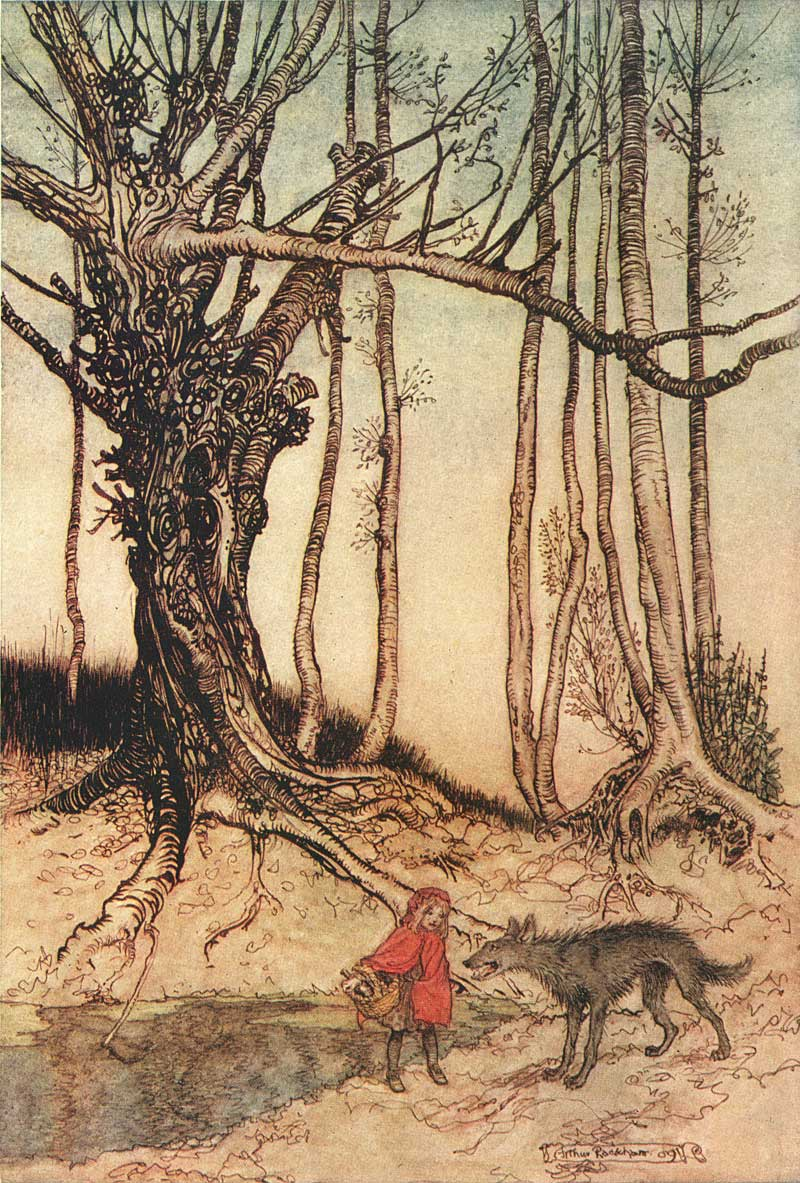
\includegraphics[width=1.5in]{littlered.jpg}
    \nbvspace[3]
    \normalsize

    \large
    PUBLISHED IN THE WILD
    \nbvspace[1]
\end{center}
\clearpage{}

    \blankpage

    \clearpage{}\newpage
\thispagestyle{plain}
\par\vspace*{.35\textheight}{\centering Dedicated to my wife, Lily Yang.\par}
\clearpage{}
    \blankpage

    \clearpage{}\chapter{Preface} \label{ch:preface}
\index{Preface@\emph{Preface}}



The main focus of this book is ``How to practice the best practices in software development?''
It comprises organic programming experiences, home-grown development techniques,
and other heartfelt coding patterns. Rather than being revolutionary, many of ideas presented in this book are small
``heartfelt engineering tips''.
However the effect of these minute engineering improvements accumulate to make a difference.
After all engineering is such a discipline that is consisted of proven, cumulative practices.


This book is also a summary of the struggles and learning, the stumbles and gains, the dark
quests and the `aha' moments recorded in my software engineering journey over the years.
By reproducing the battles I fought and sharing the insights I gained, I hope to
bridge the body of software development best practices with developers
on the industrial battle field.


Readers may find the topics in this book somewhat familiar and yet somewhat unexpected.
Most topics presented in this book lie in the gray areas where they are regularly encountered
by most developers and yet they are so elusive as to escape many developers' best practices.
As Jon Bentley put it ``This sure looks familiar \ldots but I've never seen this
before''\cite{Bentley:1986:PP}.


\section{About the author}\label{sec:whoAmI}

When my doctoral research came to a complete stall after six hard-working years, I
digging my old dreams for something else.
I was delighted to find that my passion for coding,
dormant throughout the years, is still unquenchable.
I quickly brushed it up and signed up for a semester's course in the neighboring CS Department, I
got top-of-the-class score and won a strong recommendation letter from the professor along with
two opportunities---summer internship at Microsoft and an offer letter to enroll in
the CS Department as a graduate student.
I accepted the internship but chose to stay in physics to complete my degree albeit taking two
other courses offered by the CS Department.


Then off I started my odyssey to acquire software development skills, one at a time.
It took me a decade or so to grow from a mere passionate dilettante to an experienced professional.
During this period, I read vast amount of books, articles, blog posts first on programming
primer, tools, and frameworks, then on software engineering best practices, programming paradigms,
design patterns, \textit{etc.}
I implemented most of the fundamental algorithms and data structures.
I cracked as many coding problems as I can find.
And I put them to work, which I deem as the ultimate touchstone for my learning.


But beyond these which every ambitious software developer would do,
I have a secrete weapon---I have an insatiable passion to get to the bottom
of anything that bothers me.
I periodically review my notes and reflect on my previous code just because
`something in there' upsets me.
Many of the problems that I worked on were revisited up to five or more times over the years.
Each time I was able to gain new understandings and each time my solution shrinks.


I try different solutions to solve the same problem again and again and
I keep asking myself these questions ``Why does certain implementation work or not work?
How can I improve it?''
I painstakingly dedicate quality time to think over bugs I made, bugs I fixed,
and bugs I strategically avoided.
I contemplate on new insights and attempt to reconcile it with previous experience.
I draw analogies across seemingly different fields.


Have you wondered why comparison-based sorting algorithms are unanimously bound by $O(N \log N)$?
This is one of the problems that contemplated and eventually got a psychologically
appeasing understanding.
This formula looks annoyingly familiar to me as it has a hint of statistical physics origin.
I then learned that Shannon borrowed that concept and introduced `information
entropy'\cite{Shannon-mathematical-1948}.
But how are all these connected?
Well, a shuffled array of $N$ entities encodes information and thus contains `information entropy'.
When sorted, the array is deprived of the encoded information and thus is void of entropy.
So \texttt{a} sorting algorithm to a shuffled array is like a
housekeeper to a messy room or an air conditioner to a summery building---in all three cases,
entropy is pumped out of the system into the environment.


Aha, this lights up in me.
The entropy of a thermodynamic system is logarithmic to the number of `accessible microstates'.
Now if we take the $N$-entities array as the system, then all the permutations would be
`accessible' states for the system.
Then the formula, $O(N \log N)$, suddenly makes sense
(Refer to ~\fullref{ch:timeComplexityOfSorting} for a detailed explanation).


\section{Why this book?
Why now?}\label{sec:whyThisBook}

My prolonged journey of learning and practice in the field of computer sciences was
materialized in thousands of Evernote\textregistered pages, $40,000$
lines of coding exercise on problems found online \footnote{\textit{e.g.},
\url{projecteuler.net}, \url{leetcode.com}, \url{glassdoor.com}} or offline,
and more than $100,000$ lines of production code.

I thought about writing up my adventure and learning process long ago.
But I didn't take it seriously until fairly recently when
I came across a web article talking about the then latest research report by Forrester
which claims that the prolonged shortage in software engineering talent has turned from
`lack of quantity' to `lack of quality'
\footnote{\url{https://go.forrester.com/research/predictions}}.
Quoting the article directly\footnote{Titled as ``2018's Software Engineering Talent
Shortage---It's quality, not just quantity'' on \url{https://hackernoon.com}}:
\begin{quote}
    ``The software engineering shortage is not a lack of individuals calling
    themselves `engineers', the shortage is one of quality---a lack of well-studied,
    experienced engineers with a formal and deep understanding of software engineering.''
\end{quote}


That report resonates with my own observation.
Starting about five years ago,
I started to note that many other developers, colleagues of mine included,
struggled with the same problems that I used to struggle with.
I've worked with graduates and post-graduates from top-tier schools
through numerous design reviews, code reviews, and technical interviews.
They have eye-catching GPAs.
Their resumes are full of buzz words.
They spent a great deal of time reading books on software development best practices, principles,
patterns, guidance, and advice.
But by end of the day when these best practices are to be put to production code, they
needed help.


This explains why codebases, whether proprietary or open source, whether I worked with or I
happened to come across,
are full of copy-n-pasted code that could have been avoided with a little shared function,
intricate logic that could have been simplified into a one-liner,
sneaky bugs caused by an escaped variable from its due scope,
mammoth solutions that could have been refactored into a group of lean, single-purposed functions,
and so on.
That feeling is like in a flight one glimpses duct-tape on the wing.


Browsing through fairly dense algorithmic implementations, it is not rare to see
the `smells' listed in Martin Fowler's seminal book `Refactor'~\cite{Fowler1999}.
It is shocking or even outrageous to mention but true that your mission-critical transactions
actually run on smelly code.
Nowadays ugly code has become the norm rather than exception.
As a matter of fact, if I see any code close to those in `Programming
Pearls' and its sort\cite{Bentley:1986:PP}, I would be surprised.


These plain facts convey a strong signal that there is \emph{a gap between best practices
and practicing the best practices}.
The good news is we already have an established body of `best practices'.
The bad news is that putting the `best practices' to work itself takes years of \emph{practice}.
Let's face the reality---it is a daunting task to attain the `best practices' in ones own code.
The real-world problems are usually much more complex than the toy examples used in
`best practices' books.
Unless they have first-hand empirical evidence,
developers will not \emph{feel} the values and limits of many of the `best practices';
Unless they get their hands dirty with fitting principles, design patterns and other
`best practices' into a couple of real-world projects, they would not understand the trade-offs,
collaborations, and conflicts among various `best practices'.

\begin{figure}[bth]
    \centering
    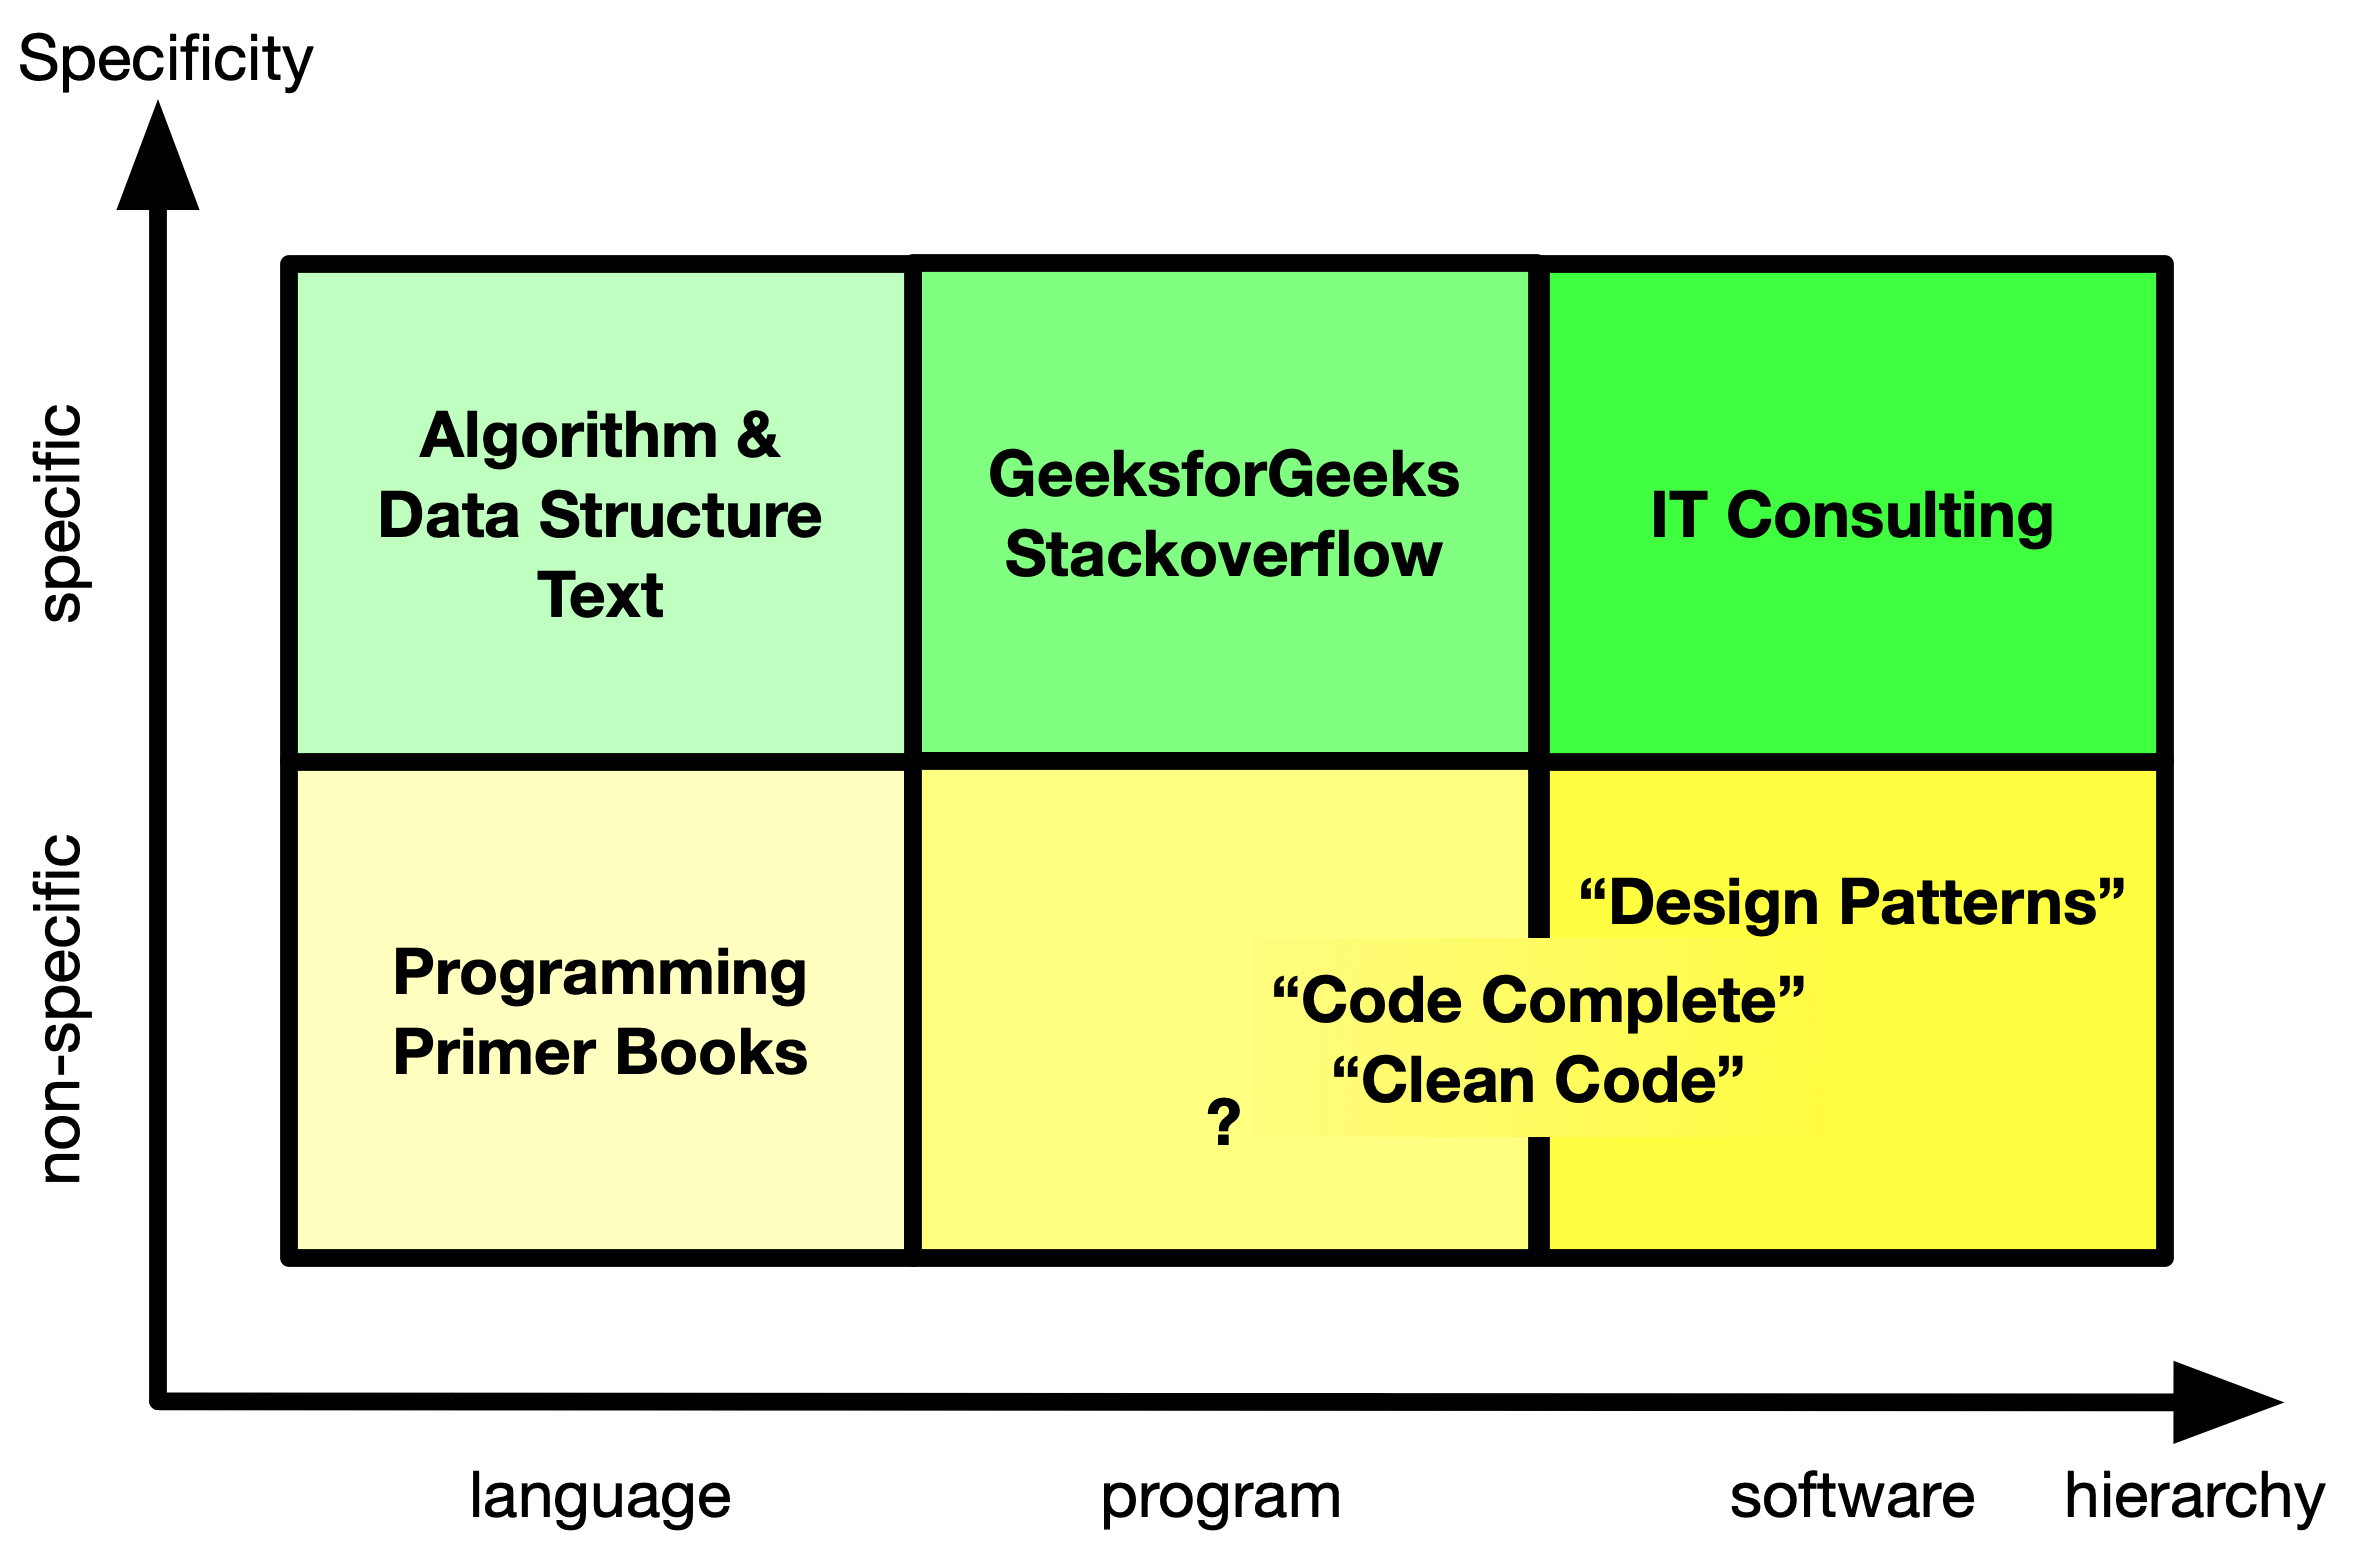
\includegraphics[width=\textwidth]{cs-spectrum.jpg}
    \caption{\label{fig:cs-spectrum} The matrix of software development expertise.
    Horizontal axis denotes the degree of application specificity;
    vertical axis is the level in software hierarchy.
    The categorization is approximate and should not be understood as clear cut.
    Instead overlapping regions exist among bordering categories.}
\end{figure}


\section{Who can benefit the most from this book?} \label{sec:whoshouldread}

Those who are striving for long-term investment of
improving their programming skills will benefit from this book the most.
Including but are not limited to data scientists who wish to sharpen their \python~ programming
skills, developers who are preparing for technical interviews, students who are thinking
seriously to pursue a career in software industry, professionals who want to solidify their coding
skills, \textit{etc.},
With that said, this book is intended for those who have had a basic understanding
of computer science.
It is assumed that readers are comfortable working with one or two of the popular
programming languages such as \python, \java, C and/or C++,
nonetheless they find it challenging to write succinct, readable, and maintainable code
in kaleidoscopic coding situations.
It is a plus but not required for reader to have knowledge in algorithm, data structure,
and/or operating system to comprehend the key ideas of this book.
Most importantly, don't be misinformed and unnecessarily daunted from reading the book.
I believe readers at all levels can find some fun parts to read.


\section{What this book is NOT about?}\label{sec:thisBookIsNotAbout}

Some disclaimers are needed here to dismiss some untrue assumptions for this book.
This book is \emph{not} a programming primer at least not systematically.
Nor does it teach you a specific programming language.


This book is not a recipe or cookbook for any specific framework or system.
Rather, it's a general guideline for development with all frameworks and systems.


Last but not least, this book is not a typical preparation material for coding interviews.
This book does not offer problem-solving strategies or
quick-n-dirty programming `tips' solely designed for coding interviews.
Coding interviews emphasize primarily on `Get it done',
whereas the focus of this book is to `Get it done right'.
As such many of the techniques presented in this book such as ~\fullref{ch:organizeYourIfElse} or
~\fullref{ch:reusableFunctions} requires more time than allowed in an interview setting.
So think of using duct-tape acceptable in interview settings while not so at work for the long-run.
Nevertheless, if the examples in this book exerts formative influence over one's coding habit and
help build up one's code sense and instinct, it would be beneficial for technical interviews
in the long run.


\section{Acknowledgement}\label{sec:acknowledgement}

A lot of people to thank\ldots


\begin{flushright}
    S.~W. @ San Mateo College Library
\end{flushright}
\clearpage{}




    \tableofcontents 

    \listoffigures

    \listoftables

    \listof{alisting}{List of algorithms}
    \listof{clisting}{List of code snippets}

    \mainmatter





    \part{\uppercase{Control Flow}}\label{prt:flowControl}

    \clearpage{}

\chapter{Reduction of Conditional Statements}\label{ch:organizeYourIfElse}

It may sound strange to you but I am going to talk about the `well-known'
commonplace---conditional statements and conditional constructs.
Supported by almost all programming languages, conditional construct is control
flow for pivoting execution path based on the on-the-fly evaluation of a boolean expression.
``Are you going to reinvent the pedestrian or what?'' you may be wondering.
Sure enough, as a universal building block, ``\code{if..else}'' is in everyone's toolbox.
In my case, about $40\%$ of my development time is spent on write
conditionals like ``\code{if..else}'' (with the another $40\%$ goes to designing loops and $20\%$
for everything else).
But it is my observation that writing optimal conditional statements and
succinct logic remains an ``advanced'' coding skill that remains a rare trait of top developers.
As a result, `working' but convoluted logic makes its way to production codebase abundantly.
Doubt it?
Let's take on a challenge---
\begin{quote}
    ``Given a \code{boolean} flag, a \code{deque}, and a \code{list}, one
    needs to pop one item from either end of the \code{deque} and append it
    to the \code{list} and the following is the rule for the pop operation:
    \begin{enumerate}
        \item if \code{flag = true}, pop from the end of the \code{deque} where the value is
        smaller;
        \item Otherwise, the one larger.
    \end{enumerate}
    Assume the \code{deque} is non-empty.''
\end{quote}
Please pause here for few minutes to think about what the code might look like before turning the
page.
\clearpage
Now let's check answers.
There are usually a variety of solutions: from commonly seen solution
\lstinputlisting[firstline=2,lastline=11]{if-else/test1_test2_append.py}
to a one-liner.
\lstinputlisting[firstline=14]{if-else/test1_test2_append.py}
Hopefully the difference is obvious to you.
This shows the huge difference between `good' and `great' solutions.
If you haven't made it a habit to strive for the `great' code, do not panic.
I did not come up with the second solution from vacuum.
Instead, I came up with the first one and by following a procedure, I `turned' it into the second
one.
This chapter is dedicated to the `How' question.


``As long as it works, who cares if the logic is the simplest?'' some may insist.
Take a look at the following code snippet, adapted and anonymized from a real example.
Suppose you are tasked to modify, refactor, and modularize it into reusable functions for a library,
do you care?
\lstinputlisting{if-else/switching-smell-code-snippet.py}

Maybe this example is a little bit too extreme.
But `barely working' solution, if it works at all, often contains code that is buggy, brittle,
verbose, and/or smelly.
It is like fat deposited over time, sooner or later they will get in your way.
Steve McConnell said ``..the primary audience [of computer programs] is made up of humans,
not computers\cite{Mcconnell.2004}.''
Martin Fowler puts it even more straightforward
``Any fool can write code that a computer can understand.
Good programmers write code that humans can understand\cite{Fowler1999}.''
So first it is an inefficient way of communication to other programmers.
Even worse, it will later become the roadblock for code refactor and reuse.
Hazy conditional condition often results in redundant/duplicate code.
Gradually your business will be derailed from fast iteration due to the friction caused by
long-standing technical debts.

In this chapter, you are going to live through processes that turn bloated conditionals
into simple logic.
You will be exposed to plenty of examples and demonstrations on how to produce beautiful,
succinct solution with simple techniques and due diligence.
You will learn to how to avoid redundancy condition checking,
short-circuit evaluation and its application, how to restrain variable scopes, \textit{etc.}
You will gain skills that will routinely help you optimize your code from `good' to
`great'.






\section{Strive for simpler conditional expressions}\label{sec:logicEquivalences}


Establishing the equivalence between logic and conditional statements can be subtle.
Simplifying them is even harder, especially when camouflaged in the
jungle of real-world code with long variable names, complex expression, comments, \textit{etc.}
Take a look at ~\autoref{lst:if-return-boolean-real-world}.
At least to me, it is not yet clear how to simplify the logic or even what it does.
\begin{clisting}
    \lstinputlisting[caption={Code snippet for demonstration},
    label={lst:if-return-boolean-real-world}]
    {if-else/equivalent_statements_if_return_real_world.java}
\end{clisting}
But if we replace the conditional expression with \code{<test>} and filter out the
comments, it becomes ~\autoref{lst:if-return-boolean} and then
it is clear that the code performs a test and returns a boolean value accordingly.
You may even realize that it is actually equivalent to ~\autoref{lst:simplified-return-boolean}.
\begin{clisting}
    \begin{minipage}[t]{.45\textwidth}
        \lstinputlisting[caption={Unsimplified test},
        label={lst:if-return-boolean},
        firstline=1,lastline=4]
        {if-else/equivalent_statements_if_return.java}
    \end{minipage}
    \hfill
    \begin{minipage}[t]{.45\textwidth}
        \lstinputlisting[caption={Simplified statement},
        label={lst:simplified-return-boolean},
        firstline=6,lastline=6]
        {if-else/equivalent_statements_if_return.java}
    \end{minipage}
\end{clisting}
But when embedded in real problems, disguised by application-specific format, style, and so on,
achieving optimal conditional programming would not be straightforward.
We therefore resort to mathematical methods to help us simplify our logic.
Many of the techniques employed in this section originates from the domain of Boolean algebra.
I frequently make references to the logical equivalences, and normal forms, truth tables,
\textit{etc.}
Review and refresh your memory on relevant materials as needed.

A boolean expression can be evaluated to two possible values---\code{true} or
\code{false}.
Depending on the evaluation result of a boolean value,
a simple conditional test as \code{if..else} may lead to one of two execution alternatives---the
\code{if}-block or the \code{else}-block;
A composite condition consisting of two boolean values makes 4 alternatives.
Three boolean values can lead to 8 alternatives.
And so on.
\begin{figure}[tb]
    \centering
    
\includegraphics[width=.7\textwidth]{if-else/nested-conditionals.jpg}
    \caption{\label{fig:conditional-branching}An example of $3$ nested conditional statements.}
\end{figure}
But in a real-world problem, not all the branches will be present or even make sense (See
~\autoref{fig:conditional-branching}).


\begin{clisting}
    \begin{minipage}[t]{.3\textwidth}
        \lstinputlisting[label={lst:nestedBranching},
        caption={v1}]
        {if-else/composite_condition_tobe_simplified.java}
    \end{minipage}\hfill
    \begin{minipage}[t]{.3\textwidth}
        \lstinputlisting[label={lst:simpleBranching},
        caption={v2}]
        {if-else/composite_condition_simplified1.java}
    \end{minipage}\hfill
    \begin{minipage}[t]{.3\textwidth}
        \lstinputlisting[label={lst:final-simplified-conditional-statement},
        caption={v3}]
        {if-else/composite_condition_simplified2.java}
    \end{minipage}
\end{clisting}
Let us examine the nested conditional, adapted from a real-world code, as shown in
~\autoref{lst:nestedBranching}.
It works but `smells'---it has complicated, nested conditional statements and duplicate
code\cite{Fowler1999}.
The readability is compromised so much so that one can hardly follow the symbolic execution paths
without some mental twists.
Nevertheless, it is a good starting point.
First let us try to eliminate the nested conditional statements.


\begin{table}[bth]
    \begin{center}
        \caption{Normal forms for conditions of execution of each statement.
        \label{tbl:breakdown-of-conditions}}
        \begin{tabular}{|l|l|}
            \hline
            code & condition to execute \\
            \hline
            statement1 & test1 $\land$ test2 \\
            statement2 & test1 $\land\lnot$ test2 $\lor\lnot$ test1 \\
            statement3 & test1 \\
            \hline
        \end{tabular}
    \end{center}
\end{table}
Observing that the \code{else} block of \code{if (test1)} is much simpler, let us flip
the logic by negating \code{test1} so that the simpler block becomes the \code{if}-block and vice
versa.
The reason for doing so will be clear in a moment.
Now we can promote the nested \code{if (test2)} up to the first-level and turn the
nested conditional statements into sequential conditional statements
that are built on top of one another like a cascade \footnote{In fact,
we just came across a pattern regarding conditional programming and
~\fullref{ch:conditional-cascade} will tell more about it.}.


The resulting code is shown in ~\autoref{lst:simpleBranching}.
As one can see, if we promote the nested conditional statement without the boolean expression
flip, the resulting code would be seriously out of balance.
Comparing with ~\autoref{lst:nestedBranching} the conditional statements in
~\autoref{lst:simpleBranching} are now streamlined and easy to understand.
But still it contains duplicate code as both \code{statement2} and \code{statement3} are repeated.


So please resist the temptation of settling and we are going to get rid of the `seemingly benign'
duplicate code.
First, let us do a back-of-envelop calculation to
obtain the sufficient and necessary conditions (SNC) for \code{statement1}, \code{statement2}
and \code{statement3}, respectively.
As shown in ~\autoref{tbl:breakdown-of-conditions},
it is clear that the key to simplify the logic lies in the conditions for the
execution of \code{statement2}.

\begin{verbatim}
    In the following \code{if-elif} block, the first condition is cumbersome and the second condition
    has some redundancy of the first.

    if sc in s2t and s2t[sc] != tc:
    return False
    elif sc not in s2t:
    s2t[sc] = tc

    This may be simplified as:

    if sc not in s2t:
    s2t[sc] = tc
    elif s2t[sc] != tc:
    return False

    There is no redundancy in condition checking also both condition expressions are simple and
    single-purposed.
\end{verbatim}

Now it is time to do some Boolean algebra.
Let $c$ be the condition for \code{statement2} to be executed and
\begin{align*}
    a &= \text{\code{test1}}, \\
    b &= \text{\code{test2}},
\end{align*}
then
\begin{align}
    c &= a \land \lnot b \lor \lnot a  \nonumber \\
    &= a \land \lnot b \lor (\lnot a \land \lnot b \lor \lnot a \nonumber) & \text{// absorption law
    }\\
    &= (a \land \lnot b \lor \lnot a \land \lnot b) \lor \lnot a \nonumber & \text{// associativity
    law}\\
    &= \lnot b \lor \lnot a & \text{// distributivity law} \nonumber \\
    &=\lnot (a \land b) & \text{// De Morgan's law} \label{eq:boolean-expression-simplify}
\end{align}
~\autoref{eq:boolean-expression-simplify} shows that the SNC for
\code{statement2} to be in the execution path
is \code{!(test1 && test2)} and this is exactly the SNC of the
\code{else}-block of the conditional statement \code{if (test1 && test2)..}.
With this hard-earned wit, it is now straightforward to implement an even simpler version as
~\autoref{lst:final-simplified-conditional-statement}.
This completes our first logic simplification process.


Another way to achieve the same goal is to use \emph{truth tables}.
Let us see how it works.
\begin{table}[h]
    \begin{center}
        \caption{True value table for \code{test1} and \code{test2}.
        \label{tbl:true-value-table}}
        \begin{tabular}{|c|c|c|}
            \hline
            \code{test1} & \code{test2} & true expr \& execution\\
            \hline
            F & F & \code{!test1} $\rightarrow$ \code{statement2} \\
            F & T & \code{!test1} $\rightarrow$ \code{statement2} \\
            T & F & \code{test1 \&\& !test2} $\rightarrow$ \code{statement2} \\
            & & \code{test1} $\rightarrow$ \code{statement3} \\
            T & T & \code{test1 \&\& test2} $\rightarrow$
            \code{statement1} \\
            & & \code{test1} $\rightarrow$ \code{statement3} \\
            \hline
        \end{tabular}
    \end{center}
\end{table}
I have constructed a truth table with \code{test1} and \code{test2} as the variables
(~\autoref{tbl:true-value-table}).
Since there are two conditional variables, there are a total four rows in the table.
Additionally, we added the third column to shows what \code{true} boolean expression leads
the execution of which statement.
Summarizing the table entries, we arrive at the following conclusions
\begin{enumerate}[label={\roman*:}]
    \item \code{statement1} is executed \emph{iff} both \code{test1} and \code{test2}
    are \code{true};
    \item \code{statement2} is executed \emph{iff} not both \code{test1} and \code{test2} are
    \code{true};
    \item \code{statement3} is executed \emph{iff} \code{test1} is \code{true}, regardless of
    \code{test2}.
\end{enumerate}
With all the mental twists untied, implementation of something like
~\autoref{lst:final-simplified-conditional-statement} naturally follows.


Thus far we have presented two processes for logic simplification.
One of them takes route of SNC for the execution of certain
statements and use that to simplify the conditional expressions.
The other starts by listing all the possible branches in a true table and looks for ways to
combine them into as few conditional expressions as possible.
In practice, you may try both.
Once you form an intuition, you will find the edge of each for certain circumstances.


To verify your understanding of the material,
~\autoref{lst:exercise-original-conditional-statement} is reserved as an exercise.
Please work it out with one or both of the two methods above and get the simplified solution as
that in ~\autoref{lst:exercise-simplified-conditional-statement}.
\begin{clisting}
    \begin{minipage}[t]{.4\textwidth}
        \lstinputlisting[label={lst:exercise-original-conditional-statement},
        caption={Simplification exercise}]
        {if-else/generic_conditioning1.java}
    \end{minipage}\hfill
    \begin{minipage}[t]{.4\textwidth}
        \lstinputlisting[label={lst:exercise-simplified-conditional-statement},
        caption={Simplified}]
        {if-else/generic_conditioning2.java}
    \end{minipage}
\end{clisting}

\subsection{Case study: Binary search with slope}\label{subsec:case-study:binary-search-direction}

Let's now consider the a real problem that we will visit and revisit in this chapter.
\begin{quote}
    Given an array of length $>= 3$, $A$, consisting of two concatenated monotonically increasing
    and decreasing portions such that \code{A[0] < A[1] < ... < A[i] > A[i+1] > A[i+2] > ... >
    A[n-1]}, write an efficient program to check if a \code{target} value exists in the array.
\end{quote}

This array is like a hill with a single ridge: in the first half, it monotonically increases until
it reaches the ridge index, \code{i}, then it monotonically decreases until the end.
It's straightforward come up with a strategy as
\begin{enumerate}
    \item finds the `ridge` index of the array
    \item Attempt to find target value in the first half before the ridge index (binary search)
    \item Attempt to find target value in the second half on or after the ridge index similarly
\end{enumerate}

\begin{clisting}
    \begin{minipage}[t]{.4\textwidth}
        \lstinputlisting[label={lst:binary-search-direction-nested},
        caption={Nested implementation of binary searching direction logic}]
        {if-else/binary_search_direction_nested.py}
    \end{minipage}\hfill
    \begin{minipage}[t]{.4\textwidth}
        \lstinputlisting[label={lst:binary-search-direction-nested},
        caption={Simplified implementation of binary searching direction logic}]
        {if-else/binary_search_direction_simplified.py}
    \end{minipage}
\end{clisting}

\section{Short-circuit evaluation}\label{sec:short-circuit-eval}

\begin{figure}[htb]
    \centering
    
\includegraphics[width=.7\textwidth]{if-else/short-circuit.jpg}
    \caption{\label{fig:short-circuit-eval}  Short-circuit evaluation of the expression tree for
    `\code{!(a||foo)&&(bar||baz)}' when \code{a=true}.
    Solid gray nodes are evaluated whereas dashed blank ones omitted.
    }
\end{figure}
Some binary logical operators, like \code{AND} and \code{OR}, have an unusual property---when
one operand assumes certain value, the final value would be deterministically fixed
regardless of the value of the other operand.
For example, if \code{a = FALSE}, then the expression `\code{a AND b}' would deterministically
evaluates to \code{FALSE}, no matter what value \code{b} assumes.
Similarly, if \code{a = TRUE}, the expression `\code{a OR b}' evaluates to
\code{TRUE} regardless.

Taking advantage of this, certain programming languages introduce
a boolean expression evaluation mechanism---namely, when the value of an expression
(or subexpressions) can be unambiguously determined, it will omit the evaluation of the
remaining part and cut short to the return value.
This is called short-circuit evaluation (SCE).
When this happens, control cuts short and returns from the expression,
thus the name `short-circuit'.
Note that SCE may be applied as many times as applicable during the evaluation of an expression.
Shown in ~\autoref{fig:short-circuit-eval} is an example where SCE is applied twice.
SCE is supported by many modern programming languages, including C, C++, \java,
\python, and others.


SCE becomes interesting and subtle when an operand has `side-effects'
besides yielding the boolean value demanded by the expression---
these `side-effects' would be \emph{no more} with the omission of the corresponding evaluation,
for better or for worse.
Here `side-effects' may refer to a diverse range of changes
that usually survive the scope of the expression---
modified variables, updated database, forms posted to websites,
or resource allocation such as \code{malloc}, page writes, disk IO, or simply elapsing time.
Because of the diversity and complexity of side-effects, inadvertent usage can easily result in
unexpected results.
Inexperienced or unwary developers may be caught by surprise.

But on the other hand, SCE may be a tool for constructing elegant logic.
Consider the following problem:
\begin{quote}
    ``Implement a method, \code{next}, to fetch the next item from a source
    (whose nature is irrelevant to this problem) and store it in a member variable
    \code{Queue cache}.
    A method \code{procure()} has been made available to fetch an element
    from the source, if any, into \code{cache}:
    \lstinputlisting{if-else/getNext_procure.java}
\end{quote}
This is an extract from a class design task that I worked on.
Presumably, the algorithm to solve this problem can be as ~\autoref{alg:fetch-element-into-cache}.
\begin{alisting}
    \caption{\label{alg:fetch-element-into-cache}}
    \begin{enumerate}
        \item Check \code{cache} to see if it is empty, if so
        \begin{enumerate}
            \item Invoke \code{procure} to populate \code{cache}
            \item If attempt is unsuccessful
            \begin{enumerate}[label={}]
                \item throw ``No element is left'' exception
            \end{enumerate}
            \item end if
        \end{enumerate}
        \item end if
        \item Return the item from the \code{cache} and clear it
    \end{enumerate}
\end{alisting}


Let us first see how to implement the algorithm in the \emph{absence} of SCE mechanism.
\lstinputlisting{if-else/getNext.java}
That is not bad, right?
The code seems pretty simple by itself.
But now that \java ~ supports SCE, so one can readily implement the following
\lstinputlisting{if-else/getNext_shortCircuit.java}
The logic is much cleaner, dwarfing the previous version without SCE\@.
How does the code work?
(Can you try to figure out that before reading on?)


When \code{cache} is full, \code{procure} will \emph{not} be invoked, by virtue of SCE
mechanism, as the conditional expression unequivocally evaluates to \code{false}.
When \code{cache} is empty, the evaluation process continues with the evaluation of
the second operand, which in turn, invokes \code{procure} and its return value determines the
overall value of the conditional expression.


Through this example, we learn the important aspects for SCE programming.
First of all, operator precedences and order of operands matters, \textit{e.i.}, \code{a && b} is
not always equivalent to
\code{b && a}, especially if the evaluation of one or both of them have side effects.
Secondly, if one seeks to consciously avoid a group of operations using SCE
mechanism based on certain condition,
one should wrap those operations in easily usable functions
with a well-defined return value of boolean type (or boolean-equivalent types).
To that end, one needs to strive for reusable, single-purposed
subroutines and modular design in general.
The `\code{procure}' function in the above problem is such an example that is compliant to the
single responsibility principle (SRP).
Last but not least, one needs to pay attention to function idempotence and mutability, among
other characteristics.
We will talk more about function design in ~\fullref{ch:reusableFunctions} and
idempotence and mutability in ~\fullref{ch:ood}.


\section{Conditional statements in a loop}\label{sec:branchinginloop}



We know that \code{break} and \code{continue} statements may be used in a loop.
Since straightforward uses of such statements in loop rarely have little practical gain,
\code{break} and \code{continue} statements are usually used within conditional blocks and this
brings both challenges and opportunities to the latter.

First, it makes logic simplification in a loop more challenging.
But it also means skilled developers have new weapons to wield for simple, succinct logic.
Let's illustrate this in the following problem
\begin{quote}
    Suppose an imaginary zoo is conducting health exams for their animal collection---insects,
    fish, birds, mammals, \textit{etc}.
    All animals will have their overall health examined;
    vertebrates will undergo radiography exams;
    temperatures are taken for warm-blooded animals;
    finally, animals in each species will have their distinct body parts examined.
    Suppose that the needed zoological and veterinary API is provided in
    module \code{zoo_veterinary_api}, including functions \code{isFish},
    \code{isInsect}, \code{checkTemperature}, \code{checkExoskeleton}, \textit{etc.}
\end{quote}


Due to the complexity of animal taxonomy, coding up a correct and elegant conditional statements
with no code duplication is not straightforward.
Some developers may introduce `slightly' duplicate code as in
\lstinputlisting{if-else/zoo_animal_health_exam_dup_code.py}
However the seemingly innocent code duplication will bite at occasions, say,
when new species such as `reptiles' or `crustaceans' join the zoo.
Some may resort to nested conditional statements such as
\lstinputlisting{if-else/zoo_animal_health_exam_nested_cond.py}
But the nested conditional statements makes the logic visually more complicated than it actually is.


Thankfully, keyword \code{continue} comes to rescue in this niche use case---\code{continue}
is meant to skip the inapplicable part of the loop body.
As shown in ~\autoref{lst:continue-in-loop-conditional}, the solution consists of evenly aligned,
compact, sequential statements, that essentially of a `cascading conditional'.
\lstinputlisting[caption={Use of \code{continue} in conditional statements in a loop.},
label={lst:continue-in-loop-conditional}]
{if-else/zoo_animal_health_exam_continue.py}
If desired, one may easily refactor the loop-body in ~\autoref{lst:continue-in-loop-conditional}
into a separate function---the only change needed is to replace
\code{continue} with \code{return} (see ~\autoref{lst:refactored-in-loop-conditional}).
\begin{clisting}[ht]
    \lstinputlisting[caption={Use of \code{return} in refactored conditional statements.},
    label={lst:refactored-in-loop-conditional}]
    {if-else/zoo_animal_health_exam_refactored.py}
\end{clisting}


Loop constructs will be discussed at length in ~\autoref{ch:loops} and ~\fullref{ch:loop-thinning}.
So we are going to stop here and defer fuller presentation there.
For a real-world application of conditional application in a loop, one may turn to
~\pageref{lst:silhouette-skyline} for the solution of the `Skyline Problem'.





\clearpage{}
    \clearpage{}

\chapter{Cascading Conditionals}\label{ch:conditional-cascade}

A sequence of three or more tightly coupled conditional statements as shown in
~\autoref{lst:simpleBranching} is probably familiar to reader.
Similar structures are not uncommon even in programing primer books.
Many times, it begins with an \code{if}-conditional, optionally followed by one or more
\code{else if} (or \code{elif}) blocks, and optionally ends with an \code{else} block.
For the sake of discussion in this book, we refer to such a train of conditional statements
collectively as `\emph{cascading conditional construct}';
sometimes we use `\emph{cascading conditional}', even simply `\emph{cascade}',
or shorthand \emph{CC}  interchangeably.

Occasionally when it is the last statement to be executed in a function
or a loop, cascading conditional may take the form of a sequence of \code{if} statements
in conjunction with \code{return}, \code{continue},
\code{break}, \code{exit}, \code{yield} and other branching statements (instead
of `\code{if..elif..elif..}').
Regardless of the form, the distinguishing characteristics of a cascading conditional are
the `tight coupling' and `sequential order' among the constituent conditional statements.
Below are some examples of cascading conditionals
\begin{clisting}[h]
    \begin{minipage}[t]{.4\textwidth}
        \lstinputlisting[label={lst:cascadeCondElif},
        caption={CC in \python}]
        {if-else/staircase_conditional.py}
    \end{minipage}\hfill
    \begin{minipage}[t]{.4\textwidth}
        \lstinputlisting[label={lst:cascadeCondReturn},
        caption={CC with keyword \code{return}}]
        {if-else/staircase_conditional_return.py}
    \end{minipage}
\end{clisting}




Cascading conditional is often used as a better alternative to nested conditionals
when facing multi-branch switching.
As ~\autoref{lst:nestedBranching} shows at the beginning of this chapter,
nested conditionals may be used for multi-branch switching.
However as the number of branches increases, nesting level as well as indentation level goes deeper.
The logic becomes unwieldy before long.
In contrast, cascading conditional offers compact logic and simple layout,
as shown in ~\autoref{lst:simpleBranching}.


Though cascading conditionals are ubiquitous in programming,
more often than not, developers' first experience with it begins with a `haphazard stumbling upon',
because seldom any systematic discussion exists to clarify the best practices surrounding it.
Used in conjunction with loops or recursive functions,
cascading conditional is an important programming construct for algorithmic implementations,
though it was not formally regarded as one in popular programming references.
For practical reasons, I am going to explain the use patterns of cascading conditional in this
section.
But rest assured that you will see its applications throughout this book---in
~\fullref{ch:loops}, ~\fullref{ch:recursion}, ~\fullref{lst:silhouette-skyline}, just to name a few.


First, let's begin with characterizing cascading conditionals.


\section{Cumulative Tests in Cascading Conditional}\label{sec:cumulativetests}

The tests in cascading conditional has cumulative effect.
To understand what this is and why, let us see how cascading conditional is executed.
Execution of a cascading conditional is analogous to stepping up a cascade.
The control successively evaluates the conditional expression and builds up the cases---the
leading conditional expression is checked and if evaluated to \code{true}, then the
first conditional block is executed and the rest is skipped;
otherwise, the next conditional expression is evaluated \ldots and so on.


As can be seen, the program acquires  assertions through tests in cascading
conditionals, as if collecting scavenger hunt stamps.
This is the essence of the `cumulative testing effect' in cascading conditionals as
illustrated in ~\autoref{lst:cascadeCondElif}.


\begin{clisting}[tbh]
    \centering
    \lstinputlisting[caption={Expanded conditionals equivalent to
    ~\autoref{lst:cascadeCondElif} (in \java)},
    label={lst:cumulative-tests-expanded-equivalent}]
    {if-else/case_stack_taken_apart.java}
\end{clisting}

One of the key advantage of using cascading conditional is to reduce the number of cases one has
to check.
This reduction in number of tests would be made clear if one expands the cascading conditional
into non-cascading conditionals.
For example, in ~\autoref{lst:cascadeCondElif} the number of tests checked is $3$
whereas in its expanded non-cascading equivalent in
~\autoref{lst:cumulative-tests-expanded-equivalent} it is $9$.
Cumulative effect saves us from retesting what's already tested and thus is one of the key factors
contributing to this test reduction.


The cumulative effect of cascading conditionals put a strict ordering among
its conditional statements.
At the same time, because of the cumulative effect, one has to commit more information in memory
at development time.
It is more challenging to keep one's mind synchronized with one's code
when programming cascading conditionals.
From this point of view, working out an expanded non-cascading equivalent such as
~\autoref{lst:cumulative-tests-expanded-equivalent} will be a useful exercise
when debugging cascading conditional in ~\autoref{lst:cascadeCondElif}.


\section{How to Arrange Conditionals in Cascading Construct}
\label{sec:orderingstaircaseconditional}

Therefore arranging the conditionals in a cascading conditional construct is the key
from every point of view.
Apparently it will take considerable deliberation in order to produce correct, optimal and succinct
cascading conditional.
It is strongly recommended that reader use due diligence to screen and arrange tests in a cascade
conditional construct.



The problem solving process goes as follows.
First, brainstorm on all the possible cases based on the project/problem requirement.
The key of this step is \emph{complete coverage} of all possibilities.
These cases may overlap with one another and which may or may not requires separate handling later.
Each problem has a unique set of conditions to be tested
which is essentially a multidimensional binary space partitioning problem\cite{NAYLOR90,NAYLOR93}.
As the cases are being tested, the solution space is also chopped in halves and
ruled out much like that of a binary search.
The BSP scheme for ~\autoref{lst:cascadeCondElif} is plotted in ~\autoref{fig:bsp}.

\begin{figure}[tb]
    \centering
    
\includegraphics[width=.6\textwidth]{if-else/binary-space-partition.jpg}
    \caption{\label{fig:bsp}A sequence of tests performs binary space partitioning.
    \code{test1} partitions the whole space $A$ into two halves (labeled as $B$ is
    the `\code{true}' space);
    \code{test2} continues to partition the other half into two halves (labeled as $C$ is
    the `\code{true}' space);
    \code{test3} then partitions the remaining half into $D$ (`\code{true}')) and $E$
    (`\code{false}').}
\end{figure}


Secondly, examine the cases and attempt to eliminate or combine unnecessary cases.
The key success index for this step is \emph{non-overlapping, non-fragmenting} cases.
For example in programming for `binary search' based algorithms, one frequently faces a trichotomy
situation: \textit{less than},\textit{equals}, or \textit{greater than}.
Usually one does not need to test all three separately.
Instead, one only need to test two of the three---\textit{e.g.}  test for \code{less than} and
\code{greater than} and if both fail then it must be the third case.
Similarly in ~\autoref{lst:lca-skew-first}, one faces the quadchotomy: both keys
located on the left subtree, on the right subtree, key \code{a} on left subtree and key \code{b} on
right, or vice versa.
But I combined the cases such that only three cases are necessary: that both keys are located on
the left, on the right, or that they straddle over the root node.


Thirdly, with the consolidated distinct cases in hand, try to discover clues
that suggest certain order for them.
The most prominent clue is the dependency graph--some test is depended by others
(like nullity check).
This would form a directed acyclic graph among the tests.
In my own experience, I rarely needed to draw a DAG for this---just a simple rule of thumb worked.
But for complicated situations it may be beneficial to do so.
So topological ordering among the tests will put a strong constraint on how we can arrange the
tests within the cascading conditional.


Another clue comes from trichotomy or quadchotomy logic as we considered in the second step.
Using the example in ~\autoref{lst:lca-skew-first} again, I first test if both keys are
located on the left or right.
If neither, then it must be the straddling case.
I did not start with the straddling case because that test is in the `middle of the thick'.
If I do it first, I still have to chase down the left and back down the right.
It is a total waste.
Generally speaking, we should start with more `exposed', more accessible `edge cases' or `corner
cases' and gradually working our way into the thick of the puzzle.


More clues may be based on convenience or convention (following left \textit{v.s.}
right branch first), performance considerations (\textit{e.g.}, postpone costly RPC calls to the
last).
You may noticed that I placed performance considerations \emph{at last}.
Yes, performance is the last thing to consider at coding time, if considered at all,
quoting Donald Knuth here ``\emph{Premature} optimization is the root of all evil in programming.''


Finally don't expect a one-pass-fix-all strategy.
More often than not, it is necessary to arrange and rearrange the conditional blocks back and forth
multiple times.
And don't forget this---after each arrangement or rearrangement, be sure to
double-check, for each line, the assumptions have been asserted by earlier tests.
The price of a missing test is either an obnoxious exception or a silently incorrect result.













\section{Tight Coupling among Conditional Statements}\label{sec:tightcoupling}

The conditional statements in a cascading conditional are usually so tightly coupled that
there is no place for foreign code remotely related to the main flow in a cascading conditional.
One drawback of the tight coupling is that developers occasionally need to create an intermediate
variable to be used in conditional expressions and
it is very inconvenient and sometimes impossible by design.
Not only that, it is also recommended that each conditional block in a cascading conditional be
simple.
It had better consist of \emph{no more than} two statements.
Anything more than that should be wrapped away as a function call.
All these restrictions and recommendations are for the purpose of code coherence and readability.

What if one desperately needs to create intermediate variables in the middle?
To demonstrate this, take a look at this problem ``Based on a list of animal's sound,
construct a list of an animal.''
The initial code snippet is as follows
\lstinputlisting[language=Java,alsolanguage=Java,]{if-else/tight_staircase_conditional.java}
Now suppose that the sounds of snakes and bees have to be amplified in order to tell them apart,
one wants to create an amplifier instance for that.
But where can one do that?
Before the cascading conditional?
That's not a good choice as it is too far away from where it will used as possible.
After all, the amplifier is not needed for any other sounds but that of snakes and bees.
Or maybe there is no snake or bee in the list and if so, creating an amplifier would be a total
waste.
In the middle just before the amplifier is needed?
For most all programming languages, the
cascade construct leaves no room for creating a new amplifier instance in the middle
\footnote{An exception is Golang where a new variable may be declared and remain visible
thereafter \emph{within} the cascading conditionals for example:
\lstinputlisting[basicstyle=\footnotesize]{if-else/intermediate_var.go}
}.

\begin{verbatim}
    \caption{This example shows how to organize the cascade if statement in natural, logical way.}
    Original
        stack = [(root, self._extract_children(root)), ...]
        while stack:
            node, children = stack[-1]
            if node.left is None and node.right is None:
                ...
            elif children:
                ...
            else:
                ...

    After optimize
        stack = [(root, self._extract_children(root)), ...]
        while stack:
            node, children = stack[-1]
            if children:
                ...
            elif node.left is None and node.right is None:
                ...
            else:
                ...
\end{verbatim}

Well, a refactor will save one from this dilemma and there are at least two ways.
First one can refactor the entire cascade into a separate function where the
coupling among the conditional statements may be made less tight
(see ~\autoref{lst:refactor_cascade_conditional}).
Secondly, one can resort to a helper function to wrap away the verbose amplification logic
(see ~\autoref{lst:modified_tight_cascade_conditional}).


\begin{clisting}
    \begin{minipage}[t]{.4\textwidth}
        \lstinputlisting[caption={Use a helper function in CC},language=Java,
        alsolanguage=Java,label={lst:modified_tight_cascade_conditional},breaklines=false]
        {if-else/modified_tight_staircase_conditional.java}
    \end{minipage}
    \hfill
    \begin{minipage}[t]{.4\textwidth}
        \lstinputlisting[caption={Refactor CC to another function},language=Java,
        alsolanguage=Java,label={lst:refactor_cascade_conditional},breaklines=false]
        {if-else/refactor_staircase_conditional.java}
    \end{minipage}
\end{clisting}

\section{Case Study}\label{sec:casestudy-cascif}


We have elaborated how to construct optimal cascade conditional above.
Let us demonstrate the effectiveness of cascading conditional through real-world use cases.
The first example is a \java~ implementation of the `\code{equals}' method with a
beautiful cascading conditional design shown in ~\autoref{lst:if-stack-equals}.
\begin{clisting}
    \lstinputlisting[label={lst:if-stack-equals},
    caption={Example implementation overriding \code{equals} in a subclass}]
    {if-else/equals.java}
\end{clisting}
Here the first condition tested is the nullity of the argument for reasons detailed previously.
Only if it survives the nullity test will the control flows on to the next condition.
Next, it is type test---checking if the object is of type `\code{MyClass}'.
These first two steps are like outposts guarding the vulnerable rest of the logic.
Only after the program endures both tests do we perform the remaining logic, \textit{i.e.}, type
cast and member variables equality checks.

From this case, you can see how the program makes its way up a `staircase', one step at a time,
marching straight through the key conditions wasting no resource on unnecessary or redundant checks.
Also you see that the cascading conditional construct in this case permits
convenient creation of intermediate variables.


Let us now consider a second example---
\begin{quote}
    ``Find the lowest common ancestor of given two keys in a binary search tree.''
    The function signature can be
    \begin{lstlisting}
        Node findAncestor(Node root, int a, int b);
    \end{lstlisting}
\end{quote}

The `lowest common ancestor' (LCA) problem has many variations and the problem we are to solve
here is a much simplified version.
Even so, the numerous special cases enticing for a special treatment can be
overwhelming to an unprepared mind.
By the nature of binary search tree, a linked data structure, and the combinations of two integers,
the number of `special' cases is large.
Among others, here is an incomplete list that bombard my head immediately:
\begin{itemize}
    \item Null BST
    \item Identical keys
    \item Duplicate keys in BST
    \item Invalid BST
    \item Skewness in BST
    \item Non-existing keys
    \item Key \code{a} on the left subtree of \code{root} and key \code{b} on the right
    (\textit{a.k.a} FLSR)
    \item Key \code{b} on the left subtree of \code{root} and key \code{a} on the right
    (\textit{a.k.a} FRSL)
    \item Two keys are on different subtrees of the \code{root} (\textit{a.k.a} STRADDLING-KEYS)
    \item Both keys on the left subtree (LEFT-SKEWED)
    \item Both keys on the right subtree (RIGHT-SKEWED)
\end{itemize}

If not designed properly, the code of handling all the cases can blow up like a nightmare.
Equipped with the techniques explained earlier, we are chilled since we know that we need to
go through the cases and eliminate some cases or renegotiate some as `non-special'.
Our worksheet is presented in ~\autoref{tbl:case-walk-thru}.
\begin{table}[bth]
    \begin{center}
        \caption{
        \label{tbl:case-walk-thru}}
        \begin{tabular}{|p{.3\textwidth}|p{.4\textwidth}|p{.3\textwidth}|}
            \hline
            Case & Description & Replacement \\
            \hline
            `Identical keys' & No special handling & N/A \\
            \hline
            `Duplicate keys in BST' & Benign, slack behavior & N/A \\
            \hline
            `Invalid BST' & BST properties assumed to hold & N/A \\
            \hline
            `Skewness in BST' & This may cause deteriorated perf but no special handling & N/A  \\
            \hline
            `FLSR' & Two keys straddling the root & complement of `LEFT-SKEWED' or `RIGHT-SKEWED' \\
            \hline
            `FRSL' & \textit{ditto} & complement of `LEFT-SKEWED' or `RIGHT-SKEWED' \\
            \hline
        \end{tabular}
    \end{center}
\end{table}
As a result, there remains a handful of distinct cases needing special handling:
\begin{itemize}
    \item Null BST
    \item Non-existing keys
    \item `STRADDLING-KEYS'
    \item `LEFT-SKEWED'
    \item `RIGHT-SKEWED'
\end{itemize}
This is certainly what we can handle with a handful of lines.


Next, let's see in what order we should arrange these cases.
Apparently, all other tests depends on a non-null \code{root}.
So obviously we should perform nullity test of root before everything else.
But What next?

First, it seems that the existence in the BST of the keys \code{a} and \code{b} may be
quite informative.
If one or the other key or both do not exist in the tree, then we can simply return \code{null}.
Alternatively, we can pursue `skewed' cases: if the two keys happen to lie on the same side of
\code{root}, we can rule out the branch on the other side---and this is doable
without first locating the keys.
Talking about `skewed' cases, another way we can do is to rule out skewness if we can prove the keys
actually `straddle' the \code{root} node.


Which test should we pursue next?
We probably don't know better until we work some examples out, at the price of implementing extra
solutions only to be thrown away.
But on the other hand, any further reasoning seems merely empty talk on the paper.
So let's pay the price and implement all three arrangements (~\autoref{lst:lca-straddle-first},
~\ref{lst:lca-skew-first}, and ~\ref{lst:lca-exist-first}).
\begin{clisting}
    \lstinputlisting[label={lst:lca-straddle-first},
    caption={Solution for LCA---identifying straddling case first'.}]
    {if-else/lca_straddle_first.java}
    \lstinputlisting[label={lst:lca-skew-first},
    caption={Solution for LCA---identifying skewness cases first'.}]
    {if-else/lca.java}
    \lstinputlisting[label={lst:lca-exist-first},
    caption={Solution for LCA---identifying existence of keys first'.}]
    {if-else/lca_existence_first.java}
\end{clisting}

By implementing the alternatives, we gain some insights.
First of all, the redundant comparisons between key values and \code{root} node value in
~\autoref{lst:lca-straddle-first} seems to indicate that
finding out if the two keys straddle the \code{root} node first does not put us
on better footing---we still have to determine if the skewness is to the left or the right
afterward.
This seems to corroborate our earlier analysis.
Maybe cases in the middle should never be the first to attack.

Secondly, identifying the existences of the keys seems independent from tracking down the
skewness of the keys and both are needed and the order can be permuted.
Code-wise, there is no apparent advantage either way.
But there is a slight advantage of determining the skewness of keys---by narrowing down the
subtree the keys are both located, if any, the search for keys will be easier.
I say `slight' in the light of a balanced BST where the search for key has logarithmic runtime
complexity.
But in the extreme case when the BST is skewed, then the performance could be a significant issue.
Do I risk of `premature optimization'?
I don't think so.
Quoting the full of Donald Knuth ``We should forget about small efficiencies,
say about $97\%$ of the time: premature optimization is the root of all evil.
Yet we should not pass up our opportunities in that critical $3\%$.''
This case probably falls squarely in the $3\%$.

So all in all, the best sequence of cases for the LCA as has been tested out is as follows:
\begin{enumerate}
    \item Nullity test for \code{root};
    \item Left skewness test;
    \item Right skewness test;
    \item Existence test for both keys;
    \item Tail case (return \code{root});
\end{enumerate}

\section{Unnest nested conditionals}\label{sec:unnestnestedconditionals}

So far we focused on producing cascading conditionals from scratch step by step.
What if one wants to refactor existing code concerning suboptimal conditional constructs?
For example, consider a code snippet where there
is a dictionary (or a \code{HashMap}) `\code{lookup}' whose key and value types are
`\code{integer}' and `\code{integer}-array', respectively.
Besides, each value is a min-heap\footnote{\url{https://en.wikipedia.org/wiki/Heap_
(data_structure)}}.
Suppose the dictionary \code{lookup} has default value filling mechanism so that
if one attempts to get value by key `\code{lookup[key]}' and the key does not exist, then the
dictionary will create a default value and put the key-value pair in the dictionary.
This is the default behavior of `\code{std::map}' in \cpp STL and
is rendered so by design in \python if the \code{dict} is created as
\begin{lstlisting}
    lookup = collections.defaultdict(list)
\end{lstlisting}
Lastly, for better or for worse, you inherited the code snippet
as in ~\autoref{lst:conditional-push-up-example} from someone else.
How would you go about with refactoring nested conditionals?
\begin{clisting}[htb]
    \lstinputlisting[label={lst:conditional-push-up-example},caption={Code snippet containing
    tint of duplicate code smell, unbalanced \code{if..else} blocks, and nested conditional},
    lastline=12]
    {if-else/nested_conditional_2_cascading_conditional.py}
\end{clisting}


Before going ahead answering the question, I'd like to make a slight diversion on the
psychological part.
Generally speaking, refactor is a risky process.
After all, no happy ending is guaranteed---the result may be better or worse.
Refactor process is, in a way, rather similar to quantum tunneling, \textit{e.g.}, electrons
`proactively dive into' energy-inhibited region, the so-called energy barrier,
in search of lower energy minima.
So one must be prepared to see that before the code gets better, it may get worse in passing.
Also one has to endure uncertainty anxiety as the result remains unknown until one come out on
the other end of the darkness.


Nevertheless, one is to overcome fear and/or laziness---`no pain no gain'.
To help cope with the hardship, I developed an `unnest' technique to convert a nested conditional
to a cascading one---for reference purposes, let us call it `test push-up'.
The technique is very simple:
First, identify tests in the nested conditionals;
Then, promote these tests to the upper level and mingle them with the other tests at that level,
that is, `test push-up'.
From here on, follow similar steps discussed in previous sections to solidify the code into a
cascading conditional.


Yeah, an example would be worth a thousand words.
Let us go through the refactor process for ~\autoref{lst:conditional-push-up-example} in detail.
First, observe that the nested \code{if} conditional is
buried in the middle of the \code{else} block and to bring it to the upper level, one risks
introducing duplicate code.
Just take note but do not be intimidated.
What compels us to move forward is overwhelmingly
strong---the nested conditional and the overly unbalanced \code{if..else} blocks thereof---and
because of that there is really no way back out for us.


So following first step in `test push-up' procedure, let's see what test is for the nested conditional.
It is not hard to see that the test is \code{len(lookup[key]) == 1}.
Here is why.
The whole block reads like this ``If after \code{heappop}, the value corresponding to the
`\code{key}' in dictionary, \code{lookup}, is empty, then evict it from the dictionary thereafter.
So no empty value is possible in the dictionary before the \code{heappop}.
Therefore the condition for the nested conditional is precisely \code{len(lookup[key]) == 1}.
So far so good.

Let us then pull it out and promote it into the upper level conditional---we now have two tests
at this level, \code{key not in lookup} and \code{len(lookup[key]) == 1}.
Alright, now follow ~\fullref{sec:orderingstaircaseconditional}
for the rest of this refactor to arrange the conditionals into a cascade.
Do not turn the page---I shut up and you code.


\clearpage
Now let's examine each other's code.
Reader might have first arrived at the following cascade conditional
\lstinputlisting[firstline=15,lastline=24]{if-else/nested_conditional_2_cascading_conditional.py}

Instead of hard, `copy-n-paste' duplication, this code block contains `soft
duplication'---hidden, `quavery', and partially duplicate code.
`Soft duplication' is often tougher to detect and remove.
The above code has repeating fragments such as `\code{heappush(...)}'.
We first introduce an intermediate variable for the argument of '\code{heappush}' operation.
Then the duplicate code becomes manifest and accessible and we can easily `factor' it out.
Finally, we get:
\lstinputlisting[firstline=28]{if-else/nested_conditional_2_cascading_conditional.py}


Through this example, I am hopeful that the reader forms a `code-sense', an instinct, and a habit
of optimization mindset.
Because awareness drives motivation,
one would be more motivated to strive for such level of neatness if one knows
what lean code looks like when facing a similar problem.
As to the threshold beyond which one would be compelled to refactor, I believe it is a
personal judgement.
So it is important for developer to establish a good judgement on when to initiate a refactor
process.
One the one hand, one should not do senseless refactor ``as soon as you spot a speckle.''
On the other, one does not want to creating or pushing off paying technical debts
by writing lousy code.
Usually when I smell `duplicate code smell' \emph{accompanied} by nested conditionals, I would
consider refactor the code to cascading conditionals.
But I would avoid writing code with `duplicate code smell' at the first place, if at all possible.


Of course, cascading conditional may not be the best solution still on occasions.
As you will learn later, the complexity of conditionals may also be designed away with
`object-oriented design'.
As it will turn out, ~\autoref{lst:conditional-push-up-example} happens to be a great
case for OOD if there is a lot of need for a light-weight counter utility class.
As to when to choose what, it will be our topic for ~\autoref{ch:ood}.
\clearpage{}
    \clearpage{}

\chapter{Strive for Lean Loops} \label{ch:loops}

As one of the most widely used programming constructs, loop is productivity
amplifier and is featured in almost all programming languages.
With a static body and nominal overheads (\textit{e.g.},
state-registering variables, \textit{etc.}), a loop can be executed as many times as desired.


A key building block as loop is, it is worth every developer's effort to master the best
practices of it.
On the opposite, it is not uncommon to spot in production code, especially algorithm-intensive code
haphazardly constructed loops, often with duplicate code dangling around.
Obviously developers who authored the haphazardly `working' code were either oblivious
with good programming practices or does not bother to spend the time on better loop constructs.



For this reason I would like to devote a substantial part of this book to clarify the best practices
concerning the construction of loops.
The major focus of this chapter is `How to avoid duplicate code?' and
`How to fix up slack loops?'
Slack loops refer to quick-n-dirty loops with duplicate code in and around it.
We will elaborate on techniques that can help one construct `lean loops'.
Once the habit of coding `lean' is formed, one will automatically, proactively seek to author high
quality code.



Another topic of this chapter is ``how to limit the scope of loop variables?''
Have you experienced that a leaky and long living loop variable is the root cause of a malicious
bug?
I am positive you are not unfamiliar with this.
Inadvertent namespace contamination often houses the most treacherous bugs.
Loop variables at large is a common cause for namespace contamination.
So when we program loops, we need to pay attention to running away loop variables.


A related topic is on the use of nested loops.
Nested loops are often a sign of suboptimal code in many circumstances.
Therefore `how not to use nested loops' is critical to reduce clutters out of one's code.
We dedicate ~\fullref{ch:embedded-loops} solely to this topic and presents techniques to help
reduce nested loops to single loop.


\section{Loop anatomy}\label{sec:loopAnatomy}



Here we will give a brief account of the parts of a loop.
We do so in a generic sense with several mainstream programming languages in mind.
First off, entering a loop is like entering a building---before one proceeds, one needs to know
where the exits are or infinite loop may result inadvertently.
For this reason, all loop constructs come with a termination test.
The location of termination test is a distinguishing feature for a loop.
Based on its location, loop constructs can be classified as \emph{pre-test}, \emph{post-test},
and somewhere in between, \emph{mid-test}.
post-test loops attempt to execute the loop body at least once no matter what.
Mid-test loops may execute part of the loop body.


Secondly, most loops have initialization sections for preparatory work.
Thirdly, as a finite-state machine, a loop construct necessarily has state updating statements
which push the loop toward its termination.
Finally there is so-called `post-loop processing', one-off processing immediately after a loop
terminates.



\begin{table}[htb]
    \begin{center}
        \caption{Loop anatomy\label{tbl:loop-construct}}
        \begin{tabular}{l|p{10cm}}
            \hline
            Component & Description \\
            \hline
            \emph{Loop initialization} &
            This is the preparatory section before the execution of a loop.
            For \code{while}-loop, this is done outside of the loop.
            In \code{for}-loop, this may be done in the \code{<init>} section of the
            \code{for}-loop construct or both.\\
            \emph{Loop test or loop condition} &
            The condition for control to enter (or continue) the loop. \\
            \emph{Loop body} &
            The block of statements to be executed in the loop. \\
            \emph{Loop state updating statements} & Almost all loops come with stateful loop
            variables.
            Updating the loop variables are important job of the loop.\\
            \emph{\code{break} statement} &
            A statement in loop body that breaks the loop and pass control to the next statement
            following the loop. \\
            \emph{\code{continue} statement} &
            A statement in loop body that interrupt the execution of the remaining
            statements in the loop.
            Note that this doesn't break the loop or pass control out of the loop. \\
            \emph{\code{return}, \code{yield}, \textit{etc.}} & These statements are
            not part of the loop construct yet they affect the control flow of the loop. \\
            \emph{Post-loop processing} &
            These are rare loop constructs, such as \code{while..else} and \code{for..else}
            in \python. \\
            \hline
        \end{tabular}
    \end{center}
\end{table}


~\autoref{tbl:loop-construct} summarizes the common parts in loop constructs of most high-level
programming languages.
On top of the standard loop constructs, possible customizations may be made with \code{break},
\code{continue}, \code{return}, \textit{etc.}, depending on the programming language of choice.
These statements blend into the loop body and fine tune the execution paths of otherwise standard
loops.


Many programming languages conveniently support more than one types of loop constructs.
\code{for}-loop and \code{while}-loop are examples of pre-test loop constructs that
almost all languages support.
\code{do-while}-loop is a post-test loop construct supported by \java, \cpp, C, and many
others (excluding \python).


Why do we need these many varieties of parts and loop constructs?
Let us illustrate the abstract concepts with concrete examples.
Say, in a cooking contest, each chef is to cook 3 dishes in a course---appetizer, main,
and desert.
Interested judges will approach the team and put an order of a full course.
Other than judge orders, chef does not cook anything else.
The competition process may be best coded with pre-test loop such as
\lstinputlisting{loop/pre_test_loop.java}


Suppose, on the last night of the competition, the rule is changed so that each chef is to cook a
course for display before judges' orders.
One can do a `copy-n-paste' to solve the problem;
or one can avoid `copy-n-paste' with a post-test loop:
\lstinputlisting{loop/post_test_loop.java}


For another example, suppose we are to develop a command line tool that takes input from
\code{stdin}.
The tool interprets user input and does a bunch of cool stuff.
It terminates when user types `exit' or simply hits `return' key
(in which case the input string is empty).
Then the best loop construct for that would be mid-test loop.
But since \java does not have a specialized mid-test loop construct, we have to makeshift by using
a \code{break} statement along with an infinite loop:
\lstinputlisting{loop/mid_test_loop.java}


\section{A word on the usage of \code{continue}, \code{break}, and \code{return}}
\label{sec:continue-and-break}

We have touched the topic in ~\fullref{sec:branchinginloop} of ~\fullref{ch:organizeYourIfElse}.
For most cases, where \code{continue} statement is used may be
equivalently realized by adding an \code{else}-clause.
But when used in a `cascading conditional' (see ~\fullref{ch:conditional-cascade}),
`\code{continue}' can simplify the loop body like a magic.
Earlier in ~\fullref{ch:organizeYourIfElse}, we illustrated the use of \code{continue} statement in
`Zoo animal health exams' problem.
At the risk of repetition, I am going to provide yet another example if only this can inspire the
reader to strive for optimal loop construction.
Suppose we are coding a game for two or more players with the following rules:
\begin{enumerate}
    \item All players take turn to enumerate natural numbers starting from $1$;
    \item When the number is divisible by $2$, the player write the number down then claps their
    hands;
    \item Otherwise when the number is divisible by $3$, the player write the number down then
    stump their feet;
    \item Otherwise when the number is divisible by $5$, the player do nothing;
    \item Otherwise the player write down the number and articulate the number loudly.
\end{enumerate}
These rules are applied in the order as they appear.
Namely, a `$10$' is not be skipped;
neither is `$15$';
but `$25$' is.

How would one solve the problem?
Without `\code{continue}', there are two obvious choices---either use composite tests such as
`\code{n \% 5 and not n \% 2 and not n \% 3}; or use nested conditionals.
Interested readers may try this on their own.
For the first choice, it involves redundant tests.
Suppose an additional rule regarding `$7$' is added, then the places to change would be doubled.
For the second choice, the readability would be compromised with the `switching
smell'\cite{Fowler1999}.
Even worse, duplicate code may chip in by repeatedly invoking `\code{result.append(i)}' for the
cases of `$2$' and `$3$', respectively.


Thankfully, an implementation using `\code{continue}' statement in conjunction
with a cascade conditional is free from any of the problems listed above:
\lstinputlisting{loop/use_of_continue.py}
It is marvelous!








Similar situations may exist for the use of \code{break}, \code{return}, \textit{etc.} to reduce
redundant code.


\section{C-style For-loop}\label{sec:for-loop}

Beside the universal \code{while}-loop, is the conventional C-like \code{for}-loop
\footnote{This is not to be confused with the iterator-based \code{foreach},
whose functionalities has largely been replaced by streaming such as in JDK 8+.},
another commonly used pre-test loop whose layout looks like looks like
\lstinputlisting{loop/for_loop.java}
The distinguishing parts of a \code{for}-loop are its header statements---the
initialization \code{<init>}, the loop test \code{<test>}, and the afterthought \code{<aftrth>}.
Below is an explanation of these header statements:
\begin{enumerate}
    \item The \code{<init>} is a statement to be executed only once as control is transferred to
    the loop.
    \item The \code{<test>} may be regarded as the \emph{first} statement of the loop body.
    \item The \code{<test>} are executed one more time than the rest of loop body
    unless loop execution is aborted with, say, \code{break}.
    \item The \code{<aftrtht>} is the afterthought statement executed at the end of each
    iteration of loop body even in the presence of \code{continue}.
    But in the presence of \code{break} statement, \code{<aftrtht>} will be skipped together with
    part of the loop body.
    \item All three header statements are optional.
    Namely, `\code{for(;;);'} is perfectly legal and represents an infinite loop.
\end{enumerate}


Design considerations for a \code{for}-loop are generally related to the header statements.
Where to update loop state?
For example, where should \code{i++} or \code{j--} be placed?
In the afterthought header or somewhere in the loop body?
How to arrange terminating statements?
Should the loop test header statement be used or use an `\code{break}' statement in the body?


All these considerations are tightly coupled and changing one will likely result in changing all.
For example it is more flexible (sometimes necessary when certain condition
has to be met to increment/decrement)
to increment/decrement state variables in loop body but it may not be the most concise form.
In a more concise loop, state updates are often done in the afterthought header statement.
For another, infinite loop is often the result of a reasoning loophole,
which causes incorrect termination condition.


To me personally, the single biggest reason to use a \code{for}-loop is its limited scope of
loop variables declared in the \code{<init>} header statements---they are invisible beyond the loop.
For example the following code wouldn't compile
\begin{lstlisting}
    for (int i = 0; i < 10; ++i) {}
    System.out.println(i); // i is undefined
\end{lstlisting}
In contrast, loop variables used by the \code{while}-loop condition have to be declared
before the loop.
Therefore they leak beyond the loop.





\section{Refactoring loops}\label{sec:refactoringLoops}

Many loops, especially those embedded in a crammed function, should be
refactored into a function just containing the loop and minimal post-loop processing logic.
Doing so not only makes the logic stand out in the original function,
but also the factored out function is compact, single-purposed, and reusable.

To eliminate of intermediate, local variables is another reason for refactoring loops into a
dedicated function.
Intermediate variables in a long function often share the same scope as the function
and thus contaminate the namespace in the latter part of the function.
Please by all means do yourself a favor and eliminate long-standing intermediate variables.
This simple thumb rule will help prevent mysterious bugs and spare you from ghost-chasing.


The following example illustrates this.
In the first version, the code in the main function \code{execute} was
misappropriated---a large part of it was usurped by the loop whose sole purpose
is to search for `a needle in the haystack'.
\lstinputlisting[lastline=12]{loop/refactor_conditional_in_loop.java}
In the following listing, we refactored the loop into a separate function.
Not only did we greatly reduced the bulging function, but most importantly
\code{target} and other intermediate variables are eliminated and
their scope are caged in the new function.
The threat of polluting the namespace in the remaining code is completely removed.
\lstinputlisting[firstline=14]{loop/refactor_conditional_in_loop.java}


\section{The `\textit{loop-and-a-half}' problem}\label{sec:loop-and-a-half-Problem}

As discussed above, when it comes to programming with loops, there are a variety of constructs
such as pre-test loop and post-test loop.
Have you wondered why we need so many varieties and families?
Is there a one-size-fit-all loop?


To answer this question, let's dig into history a bit.
In 1966, Corrado B\"{o}hm and Giuseppe Jacopini proved that \code{goto} statements are
unnecessary and programs containing them can be transformed to use only conditional statements
and loops\cite{Bohm:1966}.
Along that line of thinking, more researchers, who might have gone too far, attempted to remove
other `nuisance' in computer programming such as \code{break} and \code{return} in the middle of a
loop to reduce control flow complexity and promote code composability.
But the benefit for doing so does not pay for itself---one ends up with having to create more
intermediate variables.
one result of doing so is that more local variables are needed.
Even worse, it exacerbates problems with duplicate code in and around a loop.
This is the origin of the so-called ``Loop and a half problem''\cite{Louden-Lambert-2011}.
Today, ``\textit{loop-and-a-half} problem'' is still a pestering problem for suboptimal loop
design and implementation.


At the language level, a number of loop constructs have been introduced to
minimize the symptoms of the ``\textit{loop-and-a-half} problem''.
But that's not enough.
The burden remains with developers to choose the most suitable loop constructs.
Further, code fine-tuning is beyond simple choices of loop constructs
and must be hand-crafted at implementation time.
In the section to follow, we will introduce `loop rotation', a technique for loop
optimization that helps alleviate `loop-and-a-half' symptoms.


It may be unexpected to many.
But sentinels can also be used to cure `loop-and-a-half' problem.
We will study a few cases for this in ~\fullref{ch:sentinels} and in
~\fullref{ch:json-prettifier}.


\section{Loop Rotation}\label{sec:LoopDesignConsideration}
\begin{figure}[htb]
    \centering
    
\includegraphics[width=.7\textwidth]{loop/ferris-wheel.jpg}
    \caption{\label{fig:loop-rotation}Loop as a circular sequence.
    The nodes \code{i++} and \code{print} are candidates that can matched and coalesced into
    the loop.}
\end{figure}


Why programming loops is so hard?
For one, there are a lot of moving parts in a loop construct and need to be constructed
piece-by-piece.
For two, loop must get along with the peripheral code as well.
As you can see, a large part of the hard work for programming a loop lies outside of the loop.
All the pieces are tightly coupled together---changes in one necessitate changes in several others.


In fact, an important goal when implementing loops is to reduce duplicate code in and around
loop---be it pre-loop initialization or post-loop processing.
And one of the important techniques for it is `loop rotation'.


It is beneficial to visualize a loop construct as a Ferris wheel, a carousel, or a spool.
Mathematically speaking, a property is shared by all four---they all represent circular sequences, that is,
a sequence with rotational symmetry with respect to circular shifts.


If pictured as a Ferris wheel, distributed around the wheel are the conditional test,
initialization, state update statements and other statements in the loop body.
(see ~\autoref{fig:loop-rotation}).


\begin{figure}[htb]
    \centering
    \begin{subfigure}{.45\textwidth}
        
\includegraphics[width=\textwidth]{loop/loose-spool.jpg}
        \caption{\label{fig:loose-spool}}
    \end{subfigure}
    \begin{subfigure}{.45\textwidth}
        
\includegraphics[width=\textwidth]{loop/tight-spool.jpg}
        \caption{\label{fig:tight-spool}}
    \end{subfigure}
    \caption{\label{fig:spool-loop} If we use spool as a metaphor for loop in program, then
    `loop rotation' can be pictorially depicted as winding up loose yarns onto a spool.
    \protect\subref{fig:loose-spool}: Duplicate, sloppy code is analogous to loose, unorganized
    yarn around a spool.
    \protect\subref{fig:tight-spool}: A neat loop is analogous to a tidy spool.}
\end{figure}


Circular sequence may be cut open and mapped to a linear sequence, \textit{e.g.}, starting with
the lowest node going counterclockwise.
As if a ring may be cut open, the nodes in a circular sequence may be ordered as a linear sequence
if counting counterclockwise starting with the lowest node.
One thus may take advantage of this rotational degrees of freedom as a measure of loop fine
tuning---by `rotating' the loop to match up and coalesce duplicate code in the affinity of the loop.
We will refer to this process as `loop rotation'.


As another helpful analogy, loops are to program as spools are to yarn.
In the same way as a spool is used to organize yarn, a loop is a construct to organize program.
From this perspective, the `loop rotation' process to coalesce duplicate code is analogous to
wind up loose, messy yarn into a tidy spool (~\autoref{fig:spool-loop}).


In practice, one may first implement a prototype with unconditional \code{while (true)} or
\code{for (; ;)} loop.
This will push all the statements into the loop body for ease of `loop rotation'.
In this way, one first focuses on coming up with a working solution.
Once a working solution has been found, one can start the `loop rotation' process.
Finally, one can try different loop constructs, move and fit state-updating statements,
combine or annihilate \code{continue} and \code{break} statements, \textit{etc.}
If needed, repeat the above steps until the code is acceptable both functionally and
aesthetically.


Let us take a look at a toy example at which the `loop rotation' process can be easily applied.
It is the driving function: it creates the players, the board, the pieces, then it passes
control to the main loop, at end of the game, it presents the final result.
So here we go, the code to be improved is listed below.
\begin{clisting}[H]
    \lstinputlisting[]{loop/board_game_dupcode.py}
\end{clisting}
Looking at , as we rotate the loop, they can be aligned and coalesced line by line.
As can been seen, the last statement in the loop and the immediate statement before the loop
(lines $2$-$5$ and lines $18$-$21$ as highlighted)
are verbatim duplicate and thus may be aligned and coalesced.
So we can `roll up' the immediate statements before the loop and coalesce them with their
counterparts in the loop body.
But first of all, we need to untie the loop by `internalizing' the loop condition
so that it becomes an unconditional `\code{while(True)}' loop:
\begin{clisting}[H]
    \lstinputlisting[]{loop/board_game_dupcode-0.py}
\end{clisting}
Now watch closely---let us roll up one line:
\begin{clisting}[H]
    \lstinputlisting[]{loop/board_game_dupcode-1.py}
\end{clisting}
As you noticed, we have aligned and coalesced one line of the duplicate code.
Repeating this process $4$ more times, we would wipe out all duplicate code.
The final program looks like the following:
\begin{clisting}[H]
    \lstinputlisting[]{loop/board_game_rotated.py}
\end{clisting}
In practice you don't have to strictly go through each and every step described here.
Once you grasp the idea and become skillful, you can skip some of the intermediate steps
to quicken the process.
And you can always find your way back if you are lost.


Many times, code duplication are `soft'---two or more blocks of code are not exactly
identical but contains identical snippets or share common pattern.
We will refer to this type of hidden, quavery, and partially duplicate code as
`soft duplication'.
In contrast, we may refer to copy-n-paste code as `hard duplication'.
Comparing with hard duplication, soft duplication is tougher to detect and remove.
When dealing with soft duplication, one may perform pre-refactor to
consolidate soft duplications into hard ones and then deal with hard duplication in the normal way.


\section{Loop Initialization}\label{sec:loopInitialization}

Initialization is the preparatory code for a loop.
It is a preclude, a bridge to the loop body.
Initialization can also be deemed as a `primer coating' that prepares a substrate for the loop
body to deposit changes iteratively.


A proper initialization lays the foundation of success of the loop implementation.
A simple initialization helps reduce explicit and hidden code duplication.
More often than not, loop initialization takes simple, effortless,
intuitive values---integer $0$, empty list, zero-length string, array of simple values,
\textit{etc}.
But occasionally, initialization \code{int i = -1} may have an edge over \code{int i = 0}.
This requires one to push the boundary to achieve a simpler initialization.


As another brief example, when people think about Fibonacci sequence, they usually think it starts
with $1$:
\begin{table}[H]
    \centering
    \begin{tabular}{c|c|c|c|c|c}
        \hline
        $i$ & 1 & 2 & 3 & 4 & \ldots \\
        \hline
        $f(i)$ & 1 & 1 & 2 & 3 & \ldots \\
        \hline
    \end{tabular}
\end{table}
But add a zeroth-element to Fibonacci sequence sometimes opens new ways of thinking.
\begin{table}[H]
    \centering
    \begin{tabular}{c|c|c|c|c|c|c}
        \hline
        $i$ & 0 & 1 & 2 & 3 & 4 & \ldots \\
        \hline
        $f(i)$ & 0 & 1 & 1 & 2 & 3 & \ldots \\
        \hline
    \end{tabular}
\end{table}
Similarly, when it comes to factorial, many people starts with $1!=1$, seldom $0!=1$.
But the latter is a critical step toward the analytic expansion of the domain of factorial
functions to complex domain, in which it is known as the $\Gamma$-function.


You will see more cases later where generalization of the algorithm and/or the mathematical
concept will make the coding, and particularly initialization, easier.
Simplifying initialization process is especially important for dynamic programming.
Interested readers may skip to ~\autoref{ch:dp} to look for more information.
As in the `spiral termination' problem, sometimes looking for more general mathematical forms
means backing off from the most `intuitive' initialization and this mindset may get you in another
level of code proficiency.


In light of the `loop rotation' technique, in some cases one can take advantage of the rotational
degree of freedom of a loop to coalesce duplicate initialization
or post-loop processing code into the loop.
If you find that your initialization code actually repeats the loop body in whole or in part,
or that the post-processing logic does similar things as the loop does,
that's a sign that you should `tighten' your loop.


Loop initialization should be trivial and light-weight.
Apart from being correct, initialization should also be small.
On the other hand by design, loop body does the heavy lifting---it is responsible to progressively
mutate the initialized state to the desired final state.


Pretty simple, isn't it?
It depends.
For one who has formed a habit of striving for the simplest,
this requirement for initialization seems intuitive and natural.
But for one who is new to this, it may be a struggle
to figure out what is the correct and minimal initialization.
For example, should the initialization be \code{int i = -1} or \code{int i = 0}?


Let us take a look at the 'spiral termination problem':
\begin{quote}
    Given the dimensions of a $2$D matrix, $m$ and $n$,
    one is to visit each and every cell of the matrix in
    a clock-wise, spiral fashion from the upper left corner.
    Determine the final position when the visit finishes.
    For example, when $m=1,n=1$, it is $[0,0]$.
\end{quote}


There are more than one solutions to this problem---both iterative and recursive.
We are here to demonstrate an iterative solution with a loop.
Note that since the problem only asks for the final position,
cells passed by along the way are irrelevant.
As such, we can `hop' over cells.
Without making too much a pitch, here is an outline of the algorithm we are to implement:
\begin{quote}
    Approach the termination position in `strides'.
    In each stride, we hop over a perimetric layer of cells.
    A `perimetric layer' here consists of all the cells not yet visited but not completely
    surrounded by unvisited neighbors (see ~\autoref{fig:spiral-term-iter}).
\end{quote}


In general, if we start off at $[i,j]$ and after we finish visiting a perimetric layer,
we will finish at $[i+1,j+1]$ as shown in ~\autoref{fig:spiral-term-iter}.
\ldots Albeit for special cases when the matrix is an array (columnar or row alike).
In that case, the terminating cell is at end of the line.
For now, we are going to handle this extra complication with post-loop processing.
Altogether, apart from the to-be-determined initialization and post-loop calculation, the main loop
looks like
\lstinputlisting[]{loop/spiral_termination_todo.py}
Now all stake is laid on the initialization.
As long as that can be determined, the rest of the
code will bring it where need be.
``But what is the starting point?''


\begin{figure}[tbh]
    \centering
    
\includegraphics[width=.4\textwidth]{loop/spiral-term.jpg}
    \caption{\label{fig:spiral-term-iter}
    Iteration after one `spiral stride' in the `Spiral termination' problem.
    Purple cells denote a visited `layer'.
    Cells in red are the final positions after the first and second iterations, respectively.
    The arrow represents the final displacement from the end of first iteration
    to the end of the second.}
\end{figure}


At the first glance, initializing $i=j=0$ seems reasonable.
For example, when $m=n=3$, after `peeling off' the outer layer, \code{i,j} becomes
$[1,1]$ and indeed the process terminates on $[1,1]$.
However we will encounter problem for case $m=n=2$, for after the outer layer, our program would
end up on a eerie, non-existent cell $[1,1]$.
(The correct answer should be $[1,0]$.)

In retrospect, we are somehow one-step too further in each iteration.
This will be a problem whenever \code{min(m, n)} is an even number.
To make this work, one remedial measure is to abstain from the last iteration---it is the very
iteration that throws us off the cliff.
This is essentially applying the reverse process of `one-more iteration'
We can thus refer to this process as `one-less-iteration'.
Convince yourself that by doing so, this condition `\code{1 <= min(m, n) <= 2}' will hold true
upon loop termination and the leftover is handled in post-loop processing.
With this fix, here comes the first complete solution that works:
\lstinputlisting[]{loop/spiral_termination_final.py}
In this solution, the initialization is natural and trivial.
But still the loop condition `\code{2 < m and 2 < n}' seems little unintuitive and arbitrary.
After all, why `$2$'?


Keep in mind that this is not the only solution.
Far less so is it the best.
An straightforward thought to the `one-step-too-further' issue is ``Why not take a step back?''
Let us take a step back, literally.
Instead of thinking in terms of `the first cell of the next iteration', let us think in terms of
`the last cell in the previous iteration'.
With that mindset shift, we can flip our perspective from initializing the `starting point'
to the `finishing point'.
In other words, let \code{i, j} represents the finishing point.
For example,  $[1,0]$ is one of `the last cells of iterations' in ~\autoref{fig:spiral-term-iter}.


But the new problem is, ``Without an iteration in the first place, how do we get `the last cell of
previous iteration'?''
As a matter of fact, for a big enough matrix, [1,0] is always `the last cell of an iteration'.
But for edge cases where the matrix is not big enough, we could directly calculate and return the
result without ever hitting the loop.
So presumably, conditional statement is needed before the loop to distinguish different cases.
But keep in mind that the same logic will be needed again in post-loop logic.
Therefore if we initialize \code{i,j = 1,0}, duplicate code would be inevitable, one way or the
other.
How to proceed from here?


\begin{figure}[tbh]
    \centering
    
\includegraphics[width=.4\textwidth]{loop/spiral-term-init.png}
    \caption{\label{fig:spiral-term-init}
    `Spiral termination' problem: backtracking the initialization to an extrapolated,
    virtual cell.}
\end{figure}


At the same time, another haunting question is ``What should be returned for a $0$-sized
matrix?''
The key for both these questions lies in `backtracking' the initialization.
As shown in ~\autoref{fig:spiral-term-init}, if we extrapolate the path backwards, we would end
up on a serendipitous, virtual cell that is not part of the matrix.
Its value is, obviously, `[0,-1]'.
Should we initialize \code{i, j} to `$[0,-1]$'?


Now the situation becomes a little bit too philosophical.
On the one hand, it sounds crazy to initialize the loop variables to an invalid cell, that is not
part of any matrix.
On the other, a closer examination reveals that the virtual cell not only serves as a perfect
`sentinel' for the case of $0$-sized matrix,
in the same way as \code{null}  for the `lack of an \code{Object}',
but also makes a good initialization value that will lead to correct result and aligns well with
`Be small' requirement.
More importantly, it is the key to get rid of the duplicate code.


Without much ado, here is the iterative solution with the newly discovered initialization key:
\lstinputlisting[]{loop/spiral_termination_virtual_init.py}
This solution has an advantage over the previous in that
its input domain is larger than other---it can handle zero-sized matrices while its predecessor
cannot.
This is analogous to concept of `analytic continuation' in complex analysis if
reader is familiar with the topic.


As can be seen, changing the initialization from [0,0] to [0,-1] in between the above two solutions
is a big deal to the program.
As a result, the whole programming scenario is changed---the loop condition is changed,
the post-loop processing logic is changed.
This again explains why it is so hard to refactor a loop---the stake of inadvertently changing
its behavior or correctness is very high.


Through the `spiral termination' problem, we see that initialization plays a key role in loop
implementation.


Before we conclude this section, I want to let you know that there is a 3-liner solution to the
`spiral termination' problem:
\lstinputlisting[]{loop/spiral_termination_two_liner.py}
Or may be even simpler solutions that I don't know.
By telling you this 3-line spoiler, I am not at all telling you that your
optimization effort so far has been totally wasted.
Far from it, the information I want to convey is ``Something is built to be thrown away
at due time.''
Until that time comes, everything that exists and optimization efforts thereof are
meaningful and have their intrinsic value.


\section{Dedupe Post-loop Processing}\label{sec:one-more-cycle}

It is normal that after loop termination, non-trivial post-loop logic is needed to
transform the output to final form.
But if one finds that the post-loop code repeats certain statements in the loop body,
that is an alarm calling for code deduplication.
But if one finds that the post-loop code shares similar functionalities,
repeat certain steps in part or in whole with the loop body, one should sound the alarm.
A technique to be explained below may help you.


This technique, named `one-more-cycle', changes the loop-termination condition so that
the number of iterations in the loop is extended by one, the loop body is executed \emph{one more time}
than otherwise.
More often than not, extra logic in the loop body is needed to handle the extra iteration
slightly differently.
This is especially true if it is only soft duplication.


Again, let me illustrate the whole process with a real example.
What we will study here is the `Maximum rectangular area under
histogram' problem (problem statement is available on several sources, \textit{e.g.},
GeeksforGeeks\footnote{\url{https://leetcode.com/problems/largest-rectangle-in-histogram}}
or LeetCode\footnote{\url{https://www.geeksforgeeks.org/largest-rectangle-under-histogram}}).

The optimal algorithm for this problem is the one using an auxiliary \code{Stack<Integer>}.
For a detailed discussion of the algorithm, refer to the above mentioned sources.
Here is a brief summary of it (suppose input is an array of integers \code{heights}):
\begin{alisting}[H]
    \caption{\label{enum:stack-limited-mining-algo}Stack-based algorithm for
    the `maximum rectangular area under histogram' problem}
    \begin{enumerate}
        \item Initialize an empty \code{stack}, the whole purpose of
        which is to store indexes of an ascending subsequence of heights.
        \item Store a progressive max result initialized as \code{maxRec=0};
        \item For each \code{(index, height)} in the histogram
        \begin{enumerate}
            \item Pop all the indexes on \code{stack} whose corresponding heights are
            $\geq \mbox{\code{height}}$
            \item For each popped index \code{i}, update \code{maxRec} with the
            rectangular area formed between $[\mbox{\code{top}}, \mbox{\code{index}}]$
            with a height of \code{heights[i]}, where \code{top} is top of \code{stack}.
            (Watch out for boundary cases!) \label{itm:pop-update-maxRec}
            \item Push \code{index} onto \code{stack}.
        \end{enumerate}
        \item For each remaining index in \code{stack}, do the calculation
        as ~\ref{itm:pop-update-maxRec}, replace \code{index} with length of input array.
        \item Return \code{maxRec} as the final result.
    \end{enumerate}
\end{alisting}


Based on a random sample of submissions on LeetCode, majority of the implementations
of ~\autoref{enum:stack-limited-mining-algo} are more or less like what follows:
\lstinputlisting[]{loop/histogram_verbose.java}
While it passes $100\%$ the unit tests and was accepted by the Online Judge, this
solution has various smells.
The smelliest issue is the oversize post-process code, the entire \code{while}-loop which
is almost a verbatim repetition of the body of previous loop.
If we can get rid of this code duplication, the code quality would be greatly boosted.


The `one-more-cycle' technique is invented just for this.
Let us explain how it works.
First, extend the number of iterations in \code{for}-loop by one---instead of the loop
condition `\code{i < heights.length}', use `\code{i <= heights.length}'.
The second step is to delete the post-process \code{while}-loop.


The code as it is now does not work.
Why?
It throws `\code{ArrayIndexOutOfBoundsException}' for there is no such an element as
`\code{heights[heights.length]}'.
Once identified, it's an easy fix---we just need `extra logic' to shield
the code `\code{heights[i]}'


Shown below in ~\autoref{lst:histogram-oneMoreCycle} is
a refactored and deduped solution for the `Maximum rectangular area under
histogram' problem using the `one-more-cycle' technique.
We successfully accomplished our goal to
reduce code duplication between loop and the post-loop processing code.
\lstinputlisting[label={lst:histogram-oneMoreCycle},caption={A deduped solution for
`Maximum rectangular area under histogram' problem}]
{loop/histogram_oneMoreCycle.java}


\section{Loop Pacing}\label{sec:loop-pacing}

when it comes to optimize the construct of a loop, loop pacing is another degree of
freedom to mind and another dial to control.
Pacing refers to rate of change in loop state;
it is the dynamic aspect of a loop, representing how often loop state be updated in
respect to loop iteration.
For majority of use cases, a linearly paced loop, advancing one element per iteration, is
sufficient.
Linear pacing refers to trivial, deterministic loop update at a fixed step size for every
iteration until the end of the loop.
A typical example is the C-style \code{for}-loop: \code{for(int i=0; i<list.size(); i++)}.
Dynamically paced loop, on the other hand, refers to loop constructs that iterate
with a varying pace depending on the elements encountered.


In most cases, a linearly paced loop, iterating one element at a time, suffices
for a majority of daily use cases such as iterating through a collection.
But in situations where state updating is not evenly done with every iteration this steadily
paced loop is insufficient.
This is frequently the case in non-trivial algorithmic implementations.
Therefore dynamically paced loops finds important applications here.


For simple use cases, the usual choices can be anywhere between deterministic linear stepping
and conditional stepping.
For complex cases, the loop updating model may be like that of an automaton, a state machine.
As an extreme example of dynamic stepping, consider the `Happy number'
problem\footnote{\url{https://en.wikipedia.org/wiki/Happy_number}}:
\begin{quote}
    A happy number is defined by the following process: Starting with any positive integer,
    replace the number by the sum of the squares of its digits in base-ten,
    and repeat the process until the number either equals 1 (where it will stay),
    or it loops endlessly in a cycle that does not include 1.
    Write code to determine if a given number \code{n} is happy.
\end{quote}
\begin{figure}[htb]
    \centering
    
\includegraphics[width=.7\textwidth]{loop/happy_number.png}
    \caption{\label{fig:happy-number}The loop state, \code{n} \textit{vs.} iteration number.}
\end{figure}


This problem is relatively straightforward to solve.
In a loop, one keeps all the numbers discovered along the `path' along of the mapping from the
starting point.
When a number is detected to be repetition of an earlier one, terminate the loop.
Check if the terminating value of \code{n} is one.
A naïve implementation is as follows.
\lstinputlisting[label={lst:nonlinear-stepping},
caption={Dynamic stepping in a loop}]{loop/nonlinear_stepping_example.py}
The state of the loop is entirely encoded in the variable \code{n}.
The chart in ~\autoref{fig:happy-number} shows how the loop state changes as the program
executes for $n=7$.
Through this case, one can get a sense of how `dynamic' the pacing of a loop can be.


Trying different ways that a loop paces provides one more opportunity for it to best suit the
application.
This can be particularly helpful for `loop rotations' and compacting nested loops.
We will discuss more on this topic in ~\autoref{ch:loop-thinning}.


From the perspective of choice of loop constructs,
\code{while}-loop is more accommodating for all kinds of stepping.
for-loop, on the other hand, .
\code{for}-loop with niches for both initialization and the afterthought
statement, on the other hand, is built for steady pacing.
Unless it is for loop-variable isolation purposes, \code{for}-loop is not recommended for
dynamically paced construct.
On the other hand, if used \code{for}-loop in programs, tuning the pace of iteration may be as
simple as relocating the state-updating statements, \textit{e.g.},
from an afterthought statement to the loop body.
There is an unsaid convention regarding C-style \code{for}-loop---when the loop paces linearly
with a simple loop-state updating statement, it should be placed in the afterthought section of
the loop header.
Conversely, when you see the afterthought part missing, it should be a sign for dynamic
pacing.


\section{Conclusion}

The best practice when it comes to programming loops is to get a \emph{working version} (WV).
Once you get a WV, you can start to iterate for improvements:
duplicate code of any severity, excessive customization such as \code{break} or \code{continue}
\textit{etc}.
Try the techniques we talked about in this chapter such as `loop rotation',
`one-more-cycle', initialization reduction techniques, \textit{etc.}
Try on different loop constructs and so on.
Also keep in mind opportunities of using sentinels for certain niched applications (see
~\autoref{ch:sentinels}).
Finally, narrow down to a loop construct
that is a close match to your programming requirement
minimal loop customization, if needed at all.
The ultimate goal is to minimize or eliminate duplicate code in and around loop.

\clearpage{}
    \clearpage{}

\chapter{Case Study: $N$ Queens}\label{ch:n-queens}

\lstinputlisting[]{loop/word_breaker.py}
\lstinputlisting[]{loop/word_breaker_other_imp.py}


\section{Solution}
Our solution is backtracking.
We are going to iterate through the solutions in digital-clock order.
We place the first queen at the first possible position.
If current placement is feasible, we keep exploring the current solution space.
If we encountered dead-end, we backtrack to previous working solution by removing the last queen.
If our first queen is moved off board (at position 0), then we are done with iteration.

This is similar to the `next permutation' problem.


\lstinputlisting[label={lst:OldNQueensSolution},
caption={Count the number of solutions for the `$N$-queens' problem.}]
{case-study/n-queens/NQueens_old.java}

After refactor to better SRP and shrunk parameter list for functions \code{place()} and
\code{check()}.

\lstinputlisting[label={lst:NQueensSolution},
caption={Refactored code based on ~\autoref{lst:OldNQueensSolution} for the `$N$-queens' problem.}]
{case-study/n-queens/NQueens.java}

If one want to list solutions instead of counting them, the changes I made on top of the
~\autoref{lst:NQueensSolution} are shown in ~\autoref{lst:NQueensSolutionListSolutions}.

\lstinputlisting[label={lst:NQueensSolutionListSolutions},
caption={List solutions for the `$N$-queens' problem.}]
{case-study/n-queens/NQueensListSolutions.java}
\clearpage{}
    \clearpage{}

\chapter{Avoid Nested Loops} \label{ch:loop-thinning}

We have laid the foundation about loop programming in ~\autoref{ch:loops}.
In this chapter, we are going to address another common misbelief about nested loops---using
nested loop where it should have been avoided.
Although permitted by most programming languages, nested loops almost always bring about
hindrance to code readability.
Occasionally, inadvertent usage of nested loops even becomes the cause of degenerate runtime for
suboptimal implementations---namely, what could have been $O(N)$ becomes $O(N^2)$.


The difficulty of adopting a new programming habit in this regard is
awareness---when compelled to use a nested loop, developers need to take a step back
and think over the options.
When it comes to algorithmic implementation using nested loops, the rule of thumb is ``Be cautious'.
More often than not, nested loops are not necessary and can be compressed into single-layer,
dynamically paced loops with the help of auxiliary data structures, cascade conditionals, and so on.


The only scenario where one may find sound usage for nested loops is iterating through $2$D or
higher dimensional data structures like list of lists, matrices, \textit{etc.}
With an pair of indexes \code{int i=0, j=0}, a nested loop
has become the commonplace for iterating through a matrix.
Whether or not nested loop is the best practice is still arguable that even in such cases.
I found this is confusing as to which index is for which dimension.
It is at least an alternative to refactor the inner loop into a separate, dedicated
function with a self-explaining function name, better code encapsulation and cohesion.
Some may argue that function invocation overhead may hurt performance especially inside a loop.
My response to that is that performance is not the main concern here, \emph{yet}.
Holding up multiple goals at once will likely get us closer to none.
When performance becomes the pursuit, there are often solutions, such as vectorization for
matrix operations.



\section{Empirical Loop-thinning Technique}\label{sec:loop-thinning-technique}


Many situations that nested loops appear so compelling or even inevitable are not so
in retrospect.
We are going to present techniques that help guide one to coalesce nested loops
into a single loop in certain scenarios, which we
generally refer as `loop thinning' technique.
One particular case whose success is almost guaranteed is a type of nested loops where
the outer loop represents an evenly-paced, end-to-end iteration over a data structure whereas
on the inner loop is performed a lookup on an auxiliary data structure or
a `sliced view' of the same data structure.



Cramming all the functionalities of nested loops into one loop is hard by definition.
As a price, `nested loop thinning' process almost always
results in one or more of these changes to the body of the final loop:
\begin{itemize}
    \item extra conditional constructs are added
    \item extra tests are added to existing conditional constructs
    \item the pacing of the resulting loop is made more dynamic
    \item more boundary condition handling logic is added
    \item auxiliary data structure, such as queue or stack, is added.
\end{itemize}



\begin{figure}
    \centering
    
\includegraphics[width=0.6\textwidth]{embedded-loops/segment-for-loop-thinning.jpg}
    \caption{\label{fig:segment-for-loop-thinning} Sectioning of loop body statements
    for `loop thinning' process.
    Each section receives different treatment during the `loop thinning' process.}
\end{figure}
For the sake of argument, the body of the outer loop is
divided into three sections---\emph{pre-inner-loop} section, \emph{inner-loop} section, and
\emph{post-inner-loop} section---depending on their relative position
in respect to the inner loop (shown in ~\autoref{fig:segment-for-loop-thinning}).


The gist for flattening nested loops is as follows.
First, we need to move pre-loop statements out of the way.
To that end, use `loop rotation' technique (see ~\fullref{ch:loops}) backward
to unwind the pre-loop statements.
The second step depends on the inner loop construct.
If the inner loop has a \emph{non-trivial loop condition}, then the inner loop can
be converted to a conditional construct as-is by keyword swapping: \code{while} $\rightarrow$
\code{if}.
At the same time, the post-inner-loop statements shall be wrapped away in a piggybacking
\code{else}-clause.
On the contrary, if the inner loop is \emph{unconditional}, chances are that
there is a conditional \code{break} statement somewhere in the loop body.
Then one can tuck the post-inner-loop statements under the conditional of the
\code{break} statement replacing the latter, and the inner loop can be stripped away.


Throughout the process, please pay special attention to bypassing statements, such as
\code{break} and \code{continue}.
Regardless the venue taken, new conditional statements are inevitably formed.
one may refer to ~\fullref{ch:cascif} for best practices on how to organize effective
cascading conditionals.



Apart from the prescribed steps, some preparatory measures may be taken beforehand
to reduce the friction during the refactor process.
Where needed, compound statements may be taken apart before one wades deep.
Compound statements may get in your way of refactoring for multiple reasons.
The most obvious reason is that, well, parts of a compound statement
may end up at different places after refactoring.
Non-idempotent conditional expressions, such as \code{if (--i < 0)}, are even more lethal
because each execution of the condition ratchets the state of the loop, leaving no time for
taking a breath.
For example,
\begin{lstlisting}
    while (++i < LIMIT);
\end{lstlisting}
shall be expanded to
\lstinputlisting[]{embedded-loops/expanded-do-while.java}
before the start of loop thinning refactor.
The following Golang statement should also be unfolded beforehand:
\begin{lstlisting}
    if v := a[i]; v < LIMIT
\end{lstlisting}


For similar reasons, \code{for}-loop with all its header statements, should be taken apart and
converted to \code{while}-loop.
\code{while}-loop readily lends itself for `loop thinning' process, as one can
simply replace the keyword \code{while} with \code{if} at the proper time.


After `loop thinning',
aftermath changes may be performed for cleanup, convention conformation, or cosmetics.
Most importantly, following the removal of nested loops, other optimizations may become
accessible to further optimizations.
Like `Candy Crush Saga' game at a critical point, a single move may unlock a
gainful chain of reactivce moves.
This `avalanche effect' is the true value of the `loop thinning' technique.


Also note the application restrictions of the `loop thinning' process---inner loop must be directly
embedded in
outer loop with no intermediate layers;
also no bypassing statements, such as \code{break}, shall be in the pre-inner-loop section.


Most of the methods we present in this chapter are empirical, I cannot claim
universal applicability for many of them.
Instead, the techniques shall be considered on a case by case basis.
In what follows, we are going to demonstrate application of `loop thinning' technique through
a few examples adapted from real-world programming projects.


\section{Case Study: `Maximum Rectangular Area in Histogram'}
\label{sec:nested-loop-histogram}

As the first case study, let us finish a leftover project from ~\fullref{ch:loops}.
In producing the implementation as shown in snippet ~\autoref{lst:histogram-oneMoreCycle},
we removed duplicate post-loop processing code.
But the solution still looks overly complicated and messy.
What's wrong with it?
Nested loops!
Because of the nested loops, the code looks more crowded and sumptuous than it need be.
In this example, we are going to take the `loop thinning' technique for a road test.
We are going to follow closely the steps prescribed in `loop thinning' to coalesce the
nesting loops into a single loop.
The first preparatory step, converting the \code{for}-loop into a \code{while}-loop, is
straightforward and eventless.
Secondly, since there is no pre-inner-loop section, we can proceed directly with the next
step---eliminating inner loop.
To that end, we can simply replace keyword ~`\code{while}' with ~`\code{if}', using the loop
condition as is for the conditional construct.
Finally, an \code{else}-clause may be appended to the newly formed conditional statement to
house the \emph{post-inner-loop} statements, both \code{stack.push(i)} and \code{++i}, in it.
After all these are completed, the code looks like
\lstinputlisting[label={lst:histogram-coalesced-loop},
caption={Code for solving the `Maximum rectangular area under histogram' using a single loop.}]
{embedded-loops/histogram.java}


In comparison with ~\autoref{lst:histogram-oneMoreCycle}, solution in
~\autoref{lst:histogram-coalesced-loop} is much simpler and more transparent.
At a glance, one can unambiguously see its $O(N)$ runtime---for there is only one loop,
in each iteration an item is either pushed in or popped out,
and each item is subject to such operation no more than once.


Some nonessential changes may be made to make the code more compact.
For example, one may combine the two statements in the \code{else}-block into
`\code{stack.push(i++)}'.
Further, there is another category of changes that deal with excessive boundary checking,
such as
`\code{stack.isEmpty()}' and `\code{i == heights.length}'.
We will leave this to ~\fullref{ch:sentinels}.
But remember that these latter changes are optional
as they are nonessential for the `loop thinning' technique.


\section{Case Study: quicksort}\label{sec:nested-loop-quick-sort}

We will now consider another case study.
This is a classical example that was detailed by books such as `Programming
Pearls' and `Numerical Recipes'\cite{Bentley:1986:PP, NumericalRecipes:1992}.
My encounter with the code in these books completely redefined the word `simplicity'
in my dictionary.


My first implementation of the quicksort algorithm was in C based off
the traditional ``Hoare's partitioning'' scheme, as presented
in `Numerical Recipes' (minus the sentinel part).
But in what follows, I am going to present the idea in \python.


The outline of the quicksort function is as follows.
\lstinputlisting[label={lst:QuickSortOutline},language=C,
caption={An implementation of quicksort algorithm.}]
{embedded-loops/quicksort_outline.c}
where arguments \code{s} and \code{e} are the starting (inclusive) and ending (exclusive) pointers
to the array.
`\code{part}' is a recursive function whose base case is no-op, namely,
arrays with fewer than two elements.
With a pivot element randomly chosen out of the array,
a large array is partitioned into three consecutive parts: the pivot element in the middle, a
subarray on the left, and a subarray on the right.
Then the pivot element is swapped into its final position.
After this, each of the two subarrays is subject to the same function.
So on and so forth until each subarray is reduced to the base case.
At the return of the first call of the function, the entire array is left in sorted state.


As you may have noted, we emphasise that the partitioning function divides an array into three, not
two, parts---the pivot element $p$, the partition $\leq p$, and the partition $\leq p$.
This is crucial to the convergence / termination of the function.
It may be the case that one or the other of the two partitions is empty.
But even so, please remember the partitioning scheme employed in quicksort is \emph{three-way}.


With the Hoare's partitioning scheme, a tentative implementation for the function \code{part} is as
follows.
\lstinputlisting[label={lst:nestedLoopHoareMethod},language=C,
caption={Implementation of Hoare's partition scheme for quicksort.}]
{embedded-loops/quicksort_partition_sym.c}
First, we randomly select a pivot element and swap it to the beginning of the array
(ask yourself: ``why beginning of array?
Why not end?'').
Then two pointers, \code{s} and \code{e}, starting off the opposite ends of the array,
wade toward each other.
Each of them makes stop at `out-of-place' element.
When both stop, that is when a pair of `out-of-place' elements have been discovered,
a swap is performed to bring both elements to the respective partitions they belong to.
Then the pointers are back on their way toward each other once again.
So on and so forth until they meet or cross.
At that point, the pivot element (at the beginning of the array) is swapped into its final position.
Finally, a pointer pointing to this position is returned.


The above visual description of Hoare's partitioning scheme disguises the true complexity of
implementing it.
so much so that once in a while when my memory of any previous implementations becomes blurry or
totally fades away, it may take me quite a few days to implement a solution that can pass a
handful of unwitty test cases.
Thus repeated several times, I decided to summary the frequently-made bugs and produced a list of
`gotcha' as follows:
\begin{enumerate}
\item In pivot election, failure to swap pivot element to the beginning of array
    \item For the pointers \code{s} and \code{e}, there are two hesitating options:
    `check-then-increment' or `increment-then-check'.
    The first option leads to infinite loop for certain cases.
    \item Also a choice between `\code{<= pivot}' and `\code{< pivot}' for \code{s},
    `\code{>= pivot}' and `\code{> pivot}' for \code{e}.
    Incorrect choice may inadvertently cause pointer incrementation to be skipped under
    obscure circumstances which will, in turn, cause infinite loop
    (Remember that under no circumstances, should either pointer stops approaching each other in
    any outer loop iteration before they meet or cross.)
    \item\label{itm:quicksort-boundary-condition} In the second inner loop for pointer \code{e},
    failing to check boundary condition causes `out-of-boundary' exception.
    Incorrect boundary condition, such as \code{s < e}, again cause pointer \code{e} to stall
    in the middle of the right partition.
    This will cause the pivot is placed at the wrong place at the return of function.
    \item Outer loop termination logic also needs deliberation.
    The key decision to make is `where to break or return' rather than `when to break or return'.
    For ~\autoref{lst:nestedLoopHoareMethod}, the choice of location of return
    at the end of the loop body was made after quick a few failed attempts.
    \item Fail to swap the pivot element to its final position.
    This step often poses a stumbling block for beginners as well as other unsuspecting
    developers.
\end{enumerate}
In fact just to debug ~\autoref{itm:quicksort-boundary-condition} and
figure out the correct condition \code{pivot < e}, instead of \code{s < e}, took me $2$ good hours.
Also, deciding out the semantics of the function arguments in `\code{qsort}' took me
quite some deliberation before I finally got them right.


A large part of the complication of the problem comes from the fact that this implementation
consists of many parts that are highly entangled---changing one would necessitate simultaneously
changing others.
For example,
suppose we are going to change the semantics of \code{e} from exclusive to inclusive, what
would the pointer to be returned change to?
\code{s}? \code{s+1}? \code{e}? Or \code{e-1}?
Accompanying these changes, the recursive calls
\begin{lstlisting}
    qSort(s, p);
    qSort(p + 1, e);
\end{lstlisting}
also need changes.
With the choice of return value, should the recursive calls be changed to
\begin{lstlisting}
    qsort(s, p - 1)
    qsort(p + 1, e)
\end{lstlisting}
or
\begin{lstlisting}
    qsort(s, p + 1);
    qsort(p + 2, e);
\end{lstlisting}
or some other form?
The number of combinations for such changes grows exponentially as the degree of coupling increases.


This partially explains why it is so hard to correctly implement this seemingly simple partitioning
function.
On the one hand, the problem itself is complicated---the number of loose parts exceeds what our
brain can comfortably handle at once.
On the other, however, the way we approach the problem makes it harder---it is all because
we attempted to fight too many wars all at once.
The complexity of the problem is doubled, or tripled, the moment we decide to send one pointer
from each end of the array to meet somewhere in the middle.


Is there a more straightforward way to implement the quicksort algorithm?
Yes!
There is a simpler and more compact partition scheme credited to Nico Lomuto\cite{Bentley:1986:PP}.
By sending two pointers off the same end of the array, the Lomuto's partitioning scheme
successfully avoids fighting two frontiers at the same time and thus greatly simplifies the
partitioning process.


The two pointers each has a distinct task, each on its own pace.
The one running in front, so-named `frontier', is responsible to discover out-of-place elements.
The one running behind, aka, `guardian', guards the partition boundary.
When the frontier discovers an out-of-place element, the guardian pointer is incremented to make
room for it and a swap places it there.
Finally, the pivot element is swapped at the boundary place.
Notably, implementing this partitioning scheme only needs one loop
(see blow ~\autoref{lst:singleLoopLomuto}).
\lstinputlisting[label={lst:singleLoopLomuto},language=C,
caption={Implementation of Lomuto's partition scheme for quicksort.}]
{embedded-loops/quicksort_partition_asym.c}


Comparing ~\autoref{lst:nestedLoopHoareMethod} with ~\autoref{lst:nestedLoopHoareMethod},
one can't help but be surprised ``Seriously?
A single loop can replace three?''


Unlike the arduous implementation and debugging process of Hoare's,
that of the Lumoto's partitioning scheme has fewer moving parts, contains fewer surprises, and is
easier to follow.
However there is no free lunch.
The simplicity of Lumoto's quicksort comes with performance penalty
for certain cases, with one such case being large arrays with a significant amount of elements
of the same value.
In such cases,
the Lomuto's quicksort scheme tends to degrade to quadratic runtime complexity.
(Can you figure out why?)
In comparison, the Hoare's partitioning scheme is stable and
robust with respect to such cases, always performs at a steady O( N log N) expected runtime.
For this reason, Lomuto's partitioning scheme is not suitable for general-purpose libraries.


However, Lomuto's quicksort algorithm is still inspiring for its simplicity and elegance.
It is tempting to ask: ``Is there a quicksort implementation that has the simplicity of Lomuto's
\emph{and} the performance of Hoare's?''
I don't know for sure.
But with our `loop thinning' technique and other tools we developed in the last chapter and this, we
can explore a little bit to see if we can approach the above goal any closer than the existing
two schemes.
Our starting point is the Hoare's quicksort implementation of ~\autoref{lst:nestedLoopHoareMethod}.
As mentioned earlier, the trickiest part of that program is the nested loops which also consists
of the major complication.
Let us forcus on getting rid of that.



The immediate difficulty is how to take apart the densely packed conditional construct:
\begin{lstlisting}
    while(s < e && *++s < *pivot);
    while(pivot < e && *--e > *pivot);
\end{lstlisting}
The loop conditions here are unusual and awkward to handle
because both `\code{++s}' and `\code{--e}' ruthlessly ratchet the loop state forward
whenever control is passed to this line.
Namely, each evaluation of the loop condition, even if the condition evaluates to false, the
pointers `\code{s}' and `\code{e}' are still incremented.
If we use these conditions as is in the to-be conditional constructs, we would end up in a
dilemma---when we discover out-of-place elements, we would pass them without swap in the next
iteration because the program does not leave us any chance for that.


With the existing programming languages' syntaxes, we have no choice but to break
up the pre-incremental statements.
So something must be done to unfold the extraordinary loop conditions to
ordinary ones before we proceed with the rest of the `loop thinning' procedure.
As we learned in ~\fullref{ch:loops}, these loops may be converted first to
`\code{do-while} loops' such as
\lstinputlisting[language=C]{embedded-loops/quicksort_inner_loop_do_while.c}
and the latter are, in turn, converted to `\code{while} loops':
\lstinputlisting[language=C]{embedded-loops/quicksort_inner_loop_while.c}
After these changes are applied, our the partition function becomes
\lstinputlisting[language=C]{embedded-loops/quicksort_partition_sym_expanded_inner_loop.c}
You may have noticed that we have floated ~\code{--e} up in front of the first inner loop,
and this does not affect the correctness as can be verified.
The solution now seems equally messy, if not more so, as we started.
However, as you will see, this form will prove useful for the subsequent refactor step---`loop
rotation'.


Now we can proceed with the next step
of loop thinning---move the \emph{pre-inner-loop statements} out of the way.
(``Loop rotation'' is specified in ~\fullref{sec:LoopDesignConsideration}.)
After this step, the code becomes:
\lstinputlisting[language=C]{embedded-loops/quicksort_partition_sym_rotated_inner_loop.c}
We have accelerated the process by tucking the \emph{post-inner-loop statements}
resulted from the loop rotation to a conditional block.


Now we are ready with the third and most exciting step---converting inner loops to conditionals.
Now we encounter a complication that is new to us: we need to covert the second loop to an
`\code{else if}' clause of the first because the second inner loop is executed only after the first
exits.
Our final result is posted below after the conversion to conditional construct:
\lstinputlisting[label={lst:singleLoopHoarePart},language=C,escapechar=$,
caption={Implementation of partition function for Quicksort using one pointer.}]
{embedded-loops/quicksort_partition_single_loop.c}
Note that we have combined multiple statements into a compound one `~\code{swap(s++, e--)}'.



By now,
we achieved our goal of a quicksort partitioning implementation that has the simplicity of
Lomuto's and the robust performance of Hoare's.
In retrospection, we set off to test the hypothetical quest for a simple but performant
partitioning scheme that comprises the advantages of Lomuto's and Hoare's partitioning scheme.
Comparing with where we started off ~\autoref{lst:nestedLoopHoareMethod},
we implemented the Hoare's algorithm with a single loop plus
cascading conditionals as ~\autoref{lst:singleLoopHoarePart}.
In the process, we used the `loop rotation' techniques, the `loop thinning' techniques,
and skills concerning the construction of cascading conditionals from earlier chapters.
The new quicksort implementation retains the optimal runtime as Hoare's algorithm but has
comparable simplicity as that of Lomuto's.
That's almost too good to be true!
While we can make the solution simpler with the use of sentinel, we will leave that discussion to
next chapter.
However there is one change that can provide a little more saving.
If we change the semantic of ending pointer \code{e} from exclusive to inclusive, the
pre-increment before the loop (line~\ref{quicksort:pre-increment} of
~\autoref{lst:singleLoopHoarePart}) would be unnecessary.


As a byproduct of going through the detailed refactor
processes for the cases of this chapter, I want the reader to have a feeling about software
development model.
As we can see the most fruitful software development model, undoubtedly, is to come up with a
working solution first.
However shabby, messy, primitive a solution it may be, as long as it can pass a handful of unit
tests, it will be a great starting point.


Then through meticulous optimization process, for which many of the techniques we have talked
about and will be talking may be an aid, strive for straightforwardness, simplicity, and elegance.
In the course, one may discover new issues, adding new unit tests accordingly, and obtain new
solutions.
With the variety of solutions passing the same unit tests, one can often form a better
perspective regarding the solution space.
This will help one pick the most effective solution to the original problem.










\section{Case Study: ``Needle in Haystack'' Problem}\label{sec:nested-loop-pattern-matching}

In this case study, let us consider the `needle in a haystack' problem:
\begin{quote}
``Given two strings \code{needle} and \code{haystack}, search for the first occurrence of
\code{needle} in the \code{haystack}.''
\end{quote}
String matching algorithms come with various run time complexities.
There are simple string matching algorithms with quadratic runtime complexity.
There are also fairly sophisticated algorithms that enjoy `$O(M + N)$' linear runtime,
such as Boyer-Moore algorithm
\footnote{\url{https://en.wikipedia.org/wiki/Boyer-Moore_string-search_algorithm}} and
Knuth-Morris-Pratt algorithm
\footnote{\url{https://en.wikipedia.org/wiki/Knuth-Morris-Pratt_algorithm}}.


In this section, we are going to focus on
a rudimentary, naïve algorithm with a $O(MN)$ runtime with the following considerations.
For one, this algorithm is the foundation of the more advanced algorithms.
For two, this algorithm also takes considerable coding skill to be implemented correctly.
Thus it makes a great example to illustrate
the various coding techniques we have presented so far.


The naïve algorithm is outlined as follows.
\begin{alisting}
\caption{\label{alg:string-search-naive-algorithm}
A naïve algorithm for string search whose runtime complexity is $O(MN)$ where $M$ and $N$ are
the string lengths.}
\begin{enumerate}
\item For each index \code{i} in $[0, M-1]$, the index for the character array of
the `\code{haystack}'
\begin{enumerate}
\item For each index \code{j} in $[0, N-1]$, the index for the
character array of the `\code{needle}'
\begin{enumerate}
\item If characters at \code{i} and \code{j} do not match, break the inner loop
\end{enumerate}
\item If substring \code{s[i:i+j]} equals `\code{needle}', return \code{i}
\end{enumerate}
\item return -1
\end{enumerate}
\end{alisting}


Let us begin with a nested loop solution implemented in \java as follows:
\begin{clisting}
\lstinputlisting[label={lst:nestedLoop-string-search},caption={Code snippet with nested loops.}]
{embedded-loops/pattern_match_nested_loop.java}
\end{clisting}
We make this our starting point because it is the most easily thought of solution.
If this problem appears in the final exam or a coding challenge for a software engineer hiring,
chances are that you will see this a lot in the submitted works.


Before we apply the heavy-duty code simplification techniques,
it is a low-hanging fruit resulting in immediate improvement---one can safely end the search of the
`\code{needle}' when the remaining part of the `\code{haystack}' is shorter than the `\code{needle}'.
With this change, the condition for the outer loop becomes
\begin{lstlisting}
i + needle.length() <= haystack.length()
\end{lstlisting}



An improvement on the inner loop may be to resolve the awkward scope of the loop variable
\code{j}.
Currently the scope of \code{j} has to extend beyond the inner loop because
its value is needed after the loop.
There are several options to resolve this awkwardness.
One is to use the `one-more-cycle' technique (see ~\pageref{sec:one-more-cycle} for more details).
Instead of terminating at $j = N$, let it terminate at $j = N+1$ so that the last
iteration may be dedicated to return successful search result.
If done this way, the loop condition will be unnecessary as the loop is
either aborted in an earlier iteration or terminated on the $N+1$th iteration.
With these changes, the nested loop solution is shortened:
\lstinputlisting[label={lst:nestedLoop-one-more-cycle},caption={Code snippet with nested loops.}]
{embedded-loops/pattern_match_nested_loop_one_more_cycle.java}


With the handful of code tuning, we have made the code simpler and shorter.
But that's not all
We have so far gotten rid of the most commonly made implementation kinks.
Even though we achieved simplification of a few lines, that is not all.
We can simplify the implementation even further by doing away with the nested loop.


To that end, we will follow the prescriptions of `loop thinning' in
~\autoref{sec:loop-thinning-technique}.
Let us first prepare the code for the `loop thinning' process.
First off, let us convert all \code{for} loops to \code{while}-loops so as to reduce refactor
friction.
This implies that the increment statements, \code{++j} and \code{++j} are to be relocated to ends
of the corresponding loop bodies.


Then as usual, we eliminate the \emph{pre-inner-loop statements} by `loop rotation' in the
reverse sense, namely, we rotate the loop to `loosen' the program.
This will result in the statement `int j = 0' being used twice---once before the outer loop as
initialization and once at the end of the loop body to reset \code{j} to 0.
As a result, the initialization statement `\code{int j = 0}' is duplicated with one copy
at the forefront of the outer loop with the other after the last statement within the outer loop.
Also the inner loop now becomes an unconditional loop \code{while(true)}.
If you are still with me, the code now looks like this:
\lstinputlisting[escapechar=~]{embedded-loops/pattern_match_thinning_loop_intermediate_stage.java}
It is important to check and verify that this code still passes the same amount of
unit tests as ~\autoref{lst:nestedLoop-one-more-cycle} does.
This is the invariant that should be maintained at each important milestone
through a refactoring process.


Now we come to the second step of `loop thinning'.
Since the \code{break} statement in the inner loop is the only path that leads to the
execution of post-inner-loop statements, we can tuck them all under the same
conditional block wherein the \code{break} statement is.
Also, the condition for the same conditional statement is complementary to that of the
increment statement `\code{++j}', so we could shield \code{++j} in an \code{else} clause.


Hooray!
We are ready to remove the unconditional inner loop---and it is as simple as ``just strip it away''.
After this step, the code looks like this:
\lstinputlisting[]{embedded-loops/pattern_match_thinned_loop_intermediate_stage.java}
Finally as a cleanup step, the condition on line~\ref{line:haystack-needle} of the previous listing
may be absorbed into the loop condition.
Also the loop condition may be switched from
\begin{quote}
\code{i + needle.length() <= haystack.length()}
\end{quote}
to
\begin{quote}
\code{i + j < haystack.length()}
\end{quote}
The final version after this change is:
\lstinputlisting[label={lst:thinnedLoop},caption={Code snippet with nested loops.}]
{embedded-loops/pattern_match_thinned_loop.java}
without affecting correctness but made it more direct to ensure the safety of subsequent index
operation in the expression `\code{haystack.charAt(i + j)}'.

This completes the `loop thinning' process.
Looking back where we started, the latest version of implementation is both succinct and easier to
understand.


\section{Conclusion}\label{sec:loop-push-up-conclusion}




Nested loops are hard to understand and often pose obstacle to code refactor and extension.
While compelling, many usages of nested loops can be
substituted with one simple loop and the resultant code is usually much simplified.
I strongly advise the avoidance of nested loops in production code whenever possible.


The `loop thinning' technique is a tunneling mechanism by which developers can overcome
refactor barriers to discover new and exciting implementations from known ones.
Even if the resulting solutions is not guaranteed simpler, the new solutions thus discovered often
offer valuable perspectives for inspiring better coding practices.
\clearpage{}
    \clearpage{}

\chapter{Magic of Sentinels} \label{ch:sentinels}
Sentinels have been put to good use in military, mathematics, and civil engineering, long before
computer science became a science.
Particularly, sentinels hold a more prominent position in computer science,
it has become a programming philosophy.
Sentinels find widespread applications in computer engineering, architecture design,
compiler design, and programming languages.
Even in high-level programming languages, proper use of sentinels brings about
simplicity.
In this chapter we will give the reader a full exposure to sentinels through a few selected cases
of study.
We will demonstrate how the use of sentinels lead to great code simplification.
By doing so, we want to put sentinel in the toolset of the to-be software engineers and encourage
conscious and deliberate use of it.


\section{``Elephant in Cairo''}\label{sec:elephant-in-cairo}

You may have heard of ``Elephant in Cairo''.
It refers to the fictitious programming question ``how to hunt elephants in Africa''.
First published on ``Pachydermic Personnel Prediction'' ~\cite{elephant-in-Cairo:1989},
this question and the published solutions vividly illustrate the basics
behind sentinel values and we will repeat some of the discussions there.


Following is the algorithm based on the original, slightly modified for proper termination:
\begin{alisting}[H]
    \caption{\label{enum:elephant-hunt-algo-A}
    Algorithm for solving the `Elephant in Cairo' question.}
    \begin{enumerate}
        \item Go to Africa.
        \item Start at the Cape of Good Hope.
        \item Work northward in an orderly manner, traversing the continent alternately east and west.
        \item During each traverse pass,
        \begin{enumerate}
            \item Catch each animal seen.
            \item Compare each animal caught to a known elephant.
            \item Stop when a match is detected.
        \end{enumerate}
    \end{enumerate}
\end{alisting}
The above algorithm, however, may not end happily in the rare and
unfortunate case when there is no elephant in Africa and the hunters end up drowning in the
Mediterranean Sea.
To avoid the dreadful situation, one may add a check before each traversal to ensure
that to ensure that the hunters stop in time just before reaching the north end of Africa.


But an experienced computer scientist would borrow an elephant beforehand and place it
in Cairo before proceeding with elephant hunting.
Magically, no modification is needed---~\autoref{enum:elephant-hunt-algo-A} can be used as-is
except that a little post-hunting processing is needed---hunters have to inspect the animal they
caught and see if it is the elephant they placed in Cairo.
If yes, the hunting trip is a failure;
otherwise a success.
Of course at the end of the program, one always need to remember a cleanup step---bring
the placed elephant back home.


\section{The Concept of Sentinel in General}\label{sec:concept-of-sentinel}

In the above mentioned fictitious question, the elephant placed beforehand is the `sentinel value'.
It serves as two roles.
One it guarantees that ~\autoref{enum:elephant-hunt-algo-A} terminates.
Second, it guarantees that an animal is at hand when ~\autoref{enum:elephant-hunt-algo-A}
terminates.
In doing so it helps save the repeated, unnecessary termination check.
Of course at the end of the program, extra effort is needed to check
if the catch is the placed elephant.
That is the price to be paid.
But the benefit can pay off this price.


Starting from here, the more development work I do, the more generalized the
concept of sentinel becomes to me.
It goes much beyond mere savings on condition checking for termination.
Benefits of using sentinels are summarized as follows:
\begin{enumerate}
    \item\label{itm:sentinel:performance} Avoid costly condition-checking on performance-critical
    loops.
    \item\label{itm:sentinel:loop-and-a-half} Help get rid of `Loop-and-a-half' issue
    \item\label{itm:sentinel:oddball} Avoid the `Oddball solution' smell~\cite{Fowler1999}
    \item\label{itm:sentinel:ds} Act as a boundary-padding in data structures,
    such as linked list, \textit{etc}.
    \item Added as a complementary part to fit a mathematical concept
    or to form a generalized algorithm.
\end{enumerate}


To me, the benefits of sentinels are many, varied, and hard to grasp.
This remains until a day with an enlightenment, I came to realize: ``Isn't it the old ragged
symmetry that is behind all these?''
Indeed, in each and every of the aforementioned scenarios,
sentinel unanimously makes the problem at hand more symmetric.


It is easy to explain sentinel with symmetry.
But what is symmetry in non-technical terms?
Without explaining symmetry, it would be like explaining a mystery with another mystery.
Symmetry is the language behind beauty.
Why does symmetry embody beauty?
Because human brain is symmetry sucker---it constantly searches for patterns out of chaos.
Why are our brains suckers of symmetry?
Because `pattern` means order and order means fewer interruptions, irregularities, anomalies, or
surprises.
(One who works on an assembly line has a deep feeling about this.)
In the end, all of these means lower information entropy.
So by leveraging symmetry, our brains seek the most economic way to handle information and thus
conserve energy.
In summary, outwardly, symmetry is pleasing to the eye;
inwardly, it helps save energy.


Now back to the use of sentinels in programs.
It is so for human brain, so also for computer `brain'.
From \code{for}-loops to regular expressions (regex), from standardized exit codes
to \code{null} pointers, from recursion to sentinels, computer science tirelessly
pursue and take advantage of symmetry to treat things uniformly, whenever and wherever possible.
In doing so, it reduces memory footprint, saves CPU cycles, minimize energy consumption.
In doing so, it does more with less.



\begin{figure}[H]
    \centering
    \begin{subfigure}{.45\textwidth}
        
\includegraphics[width=\textwidth]{sentinels/sunflower.jpg}
        \caption{\label{fig:symmetric-flower}Symmetric sunflower seeds forms beautiful spiral
        patterns.}
    \end{subfigure}
    \begin{subfigure}{.45\textwidth}
        
\includegraphics[width=\textwidth]{sentinels/sunflower-asymm.jpg}
        \caption{\label{fig:asymmetric-flower}The missing seeds in this otherwise symmetric image
        causes irregularity and anomaly.}
    \end{subfigure}
    \caption{\label{fig:line-view}Symmetry in sunflower pedal is at peace.
    With the missing seeds, the cost to process the sunflower is elevated.}
\end{figure}


The representation of `$23:59$' as `one minute to midnight' embodies the idea behind sentinels.
Here is what it means by `one minute to midnight':
first, put in one minute to make it evenly \emph{12 o'clock am};
then when you need the time, remember to take away the minute.
The `pluses and minuses' are implied.
To many, this representation `looks cleaner' and is preferred.


This is also how sentinels work.
In the opening example, `Elephant in Cairo', an elephant was added in the beginning and
deducted at the end.
Apart from being added at the beginning and taken away at the end, sentinel values remain intact.
This is reminiscent to catalysts in chemical reactions.
Catalysts are added to accelerate reaction but they themselves are not consumed by the reaction.
For this reason, we may refer to sentinels as `the catalysts of programming'.



The mechanism of sentinels also has physical analogies.
You may have noticed that dews are often found on the surface of something---
water bottle, stone, leaves, \textit{etc.}
This is because it is much effective and faster for water vapor to condense on
the surface of a solid or liquid core.
Spontaneous condensation in gaseous phase is possible but it is so energetically costly that it
takes hours in the so-called supersaturated state for that to take place.
Water vapor in the cloud condenses more readily on some non-gaseous cores called `cloud
condensation nuclei' or CCN for short ~\cite{condensation:2005}.
The non-gaseous cores are essentially borrowed sentinels.
You see, even rain need sentinel ushers!


In practice, sentinels help shift certain operations from performance-critical
section to non-critical section, from inconvenient location to convenient
location and reduce the number of such operations from many to one.
Thanks to sentinels, one can thus optimize code to be more elegant and performant.
In the following sections, we will identify opportunities to apply the concept of sentinel through
a couple of cases of study.



\section{Case Study: quicksort}\label{sec:quick-sort-sentinel}


I came to learn about sentinels from the book ``Numerical Receipt in C''
~\cite{NumericalRecipes:1992} in the section ``Quicksort''.
It was eye-opening to see how the authors gracefully avoided the array boundary checks
with the use of sentinels.
I psychologically accepted the pitch made for sentinels while I was with the book.
Closing the book, however, I am still dubious about its plausibility until I myself have a
success implementing it.
In this section, I pick this work to make a pitch to the reader about sentinels.


For stark effect of the sentinels, we will first fix the traditional implementation of `Hoare's
partitioning' scheme from ~\fullref{ch:loop-thinning}:
~\fullref{lst:QuickSortOutline} gives the outline of the program and
~\fullref{lst:nestedLoopHoareMethod} gives a fully implemented partitioning function.
As mentioned in ~\autoref{ch:loop-thinning}, one can get involved in the thick of implementing
`Hoare's quicksort algorithm'.
Not only the problem itself is tricky but also the way we implement it.
By picking Hoare's quicksort scheme over its alternative (such as Lomuto's),
we insist on the robust $O(N log N)$ expected runtime.


We attempt to get rid of the boundary checking using sentinels.
These boundary checking are there to ensure that the pointers `\code{s}' and `\code{e}' do not slip
off the ends of the array.
In large arrays, these boundary check operations may get in the way of performance of the algorithm.
But the main reason of doing so is to remove clutter in the code.



The main idea is to make boundary checking redundant by effecting some artifacts that catch the
pointers before the `out of boundary' error happens.
This is exactly what sentinel is good at!
By deploying sought-after values, the `sentinels', at the ends of the array before the control
hits the loop, the following will happen:
\begin{enumerate}
    \item the pointers, `\code{s}' and `\code{p}', would have to stop when they hit the ends of
    array;
    \item the subsequent logic will guarantee the termination of the outer loop and
    thus guarantee the inner loop would not be executed again.
\end{enumerate}


What are the sought-after values by `\code{s}' and `\code{e}'?
The out-of-place values!
Particularly, \code{s} is looking for values that are `$\geq$ the pivot';
\code{e} is looking for values `$\leq$ the pivot'.
So then instead of randomly picking one value for pivot, we now randomly pick $3$ values, the median
of which be elected as the pivot as usual, the minimum be deployed to the left end, and the maximum
to the right end.
We group these operations into a function called `\code{init_swap}':
\lstinputlisting[]{sentinels/qsort_init_swap.c}


Now back the function `\code{part}'.
As we mentioned before, the deployment of sentinels in function `\code{init_swap}' makes
the conditional expressions `\code{s < e}' and `\code{pivot < e}' semantically redundant.
They can now be safely removed.
Below is the function `\code{part}' after all the refactoring is done.
\lstinputlisting[]{sentinels/qsort_part_sentinel.c}
Comparing with the implementation ~\autoref{lst:nestedLoopHoareMethod}, this code
cleans out clutter in the loop conditions in the inner loops.
We `float' the control all the way through the termination of the program on a `touchless' rail made
by sentinels, without ever needing to check boundary condition.
Of course, the onus is shifted to the initialization before the loop.
Comparing with the inner loops, that section is non-critical.
Not only that the code is made less cluttered, but also the number of such checks
is reduced from $O(N)$ to $O(1)$.
More importantly, by not checking boundary conditions at the most critical section,
we avoid bugs that would otherwise cost us many hours of debugging time.


So by use of sentinels on the traditional Hoare's quicksort algorithm,
we shifted the complexity among the nested loops to a non-critical part of the program,
effectively reduced its coding complexity.
Remember that we came up with a new, single-loop implementation for the Hoare's quicksort algorithm
in ~\fullref{ch:loop-thinning}, as presented in ~\autoref{lst:singleLoopHoarePart}.
Can we apply the idea of sentinel to make it even better?
Yes, it may be applied equally well.
Below is the implementation of the function `\code{part}' with a single loop and simplified
boundary condition with sentinel values.
\lstinputlisting[]{sentinels/quicksort_partition_single_loop_sentinel.c}
This brings implementations of Hoare's quicksort to the next level of simplicity.


\section{String terminating sentinels}\label{sec:stringTerminationSentinels}

Despite of controversial opinions\cite{Ritchie:1993,expensive-one-byte:2011}, the
null-terminated strings in C is another brilliant use of sentinel.
Even though saving memory is a major concern when it was originally designed, the
null-terminated string has many programming advantages.
One example is the expression \code{*p == '\0'} which test if the pointer \code{p} points to end
of the string.
Without using null character as a sentinel, it would not be so convenient to perform this test.
Null-terminated strings in other languages has been deprecated largely due to development
of containers and collections.
But the idea of it is still inspiring to us.
A coding problem `Word abbreviation problem' will help illustrate this.
The problem statement is as follows ~\footnote{Credit to Leetcode\url{leetcode.com}}:
\begin{quote}
    Given a non-empty string \code{s} of English word and an abbreviation \code{abbr},
    return whether the string matches with the given abbreviation.
    You may assume the string \code{s} consists only the 26 English alphabet with cases.
    Abbreviation of word is made if zero, one or more non-overlapping substrings
    are replaced by the length of the substring in decimal format.
    \emph{Example 1:}
    Given \code{s = "internationalization"}, \code{abbr = "i12iz4n"}:
    Return true.
    \emph{Example 2:}
    Given \code{s = "apple"}, \code{abbr = "a2e"}:
    Return false.
\end{quote}
\begin{figure}
    \centering
    
\includegraphics[width=0.3\textwidth]{sentinels/letter-number-section.jpg}
    \caption{\label{fig:letter-number-section} The word `pseudoanthropological'
    as an example for string abbreviation.}
\end{figure}
In the most obvious way, the following tasks are needed to solve the problem:
\begin{enumerate}
    \item\label{itm:breakup.letter.number} Break up the string \code{abbr} into alternating
    alphabetic groups and numeric groups;
    \item\label{itm:parse.numbers} Validate and parse the numeric groups as integers;
    \item\label{itm:skip-char} Inflating each numeric group with the corresponding number of
    wildcard characters;
    \item\label{itm:check.letters} Check if the string \code{s} and the inflated \code{abbr} match.
\end{enumerate}


Numeric group validation is where `gotchas' hide.
Since the length of non-empty substrings is positive integer,
numeric group only consists of digits $0$ - $9$.
Additionally, leading `$0$' will also render the numeric group invalid.

\begin{table}[h]
    \begin{center}
        \caption{Possible combinations
        \label{tab:letter-number-combination}}
        \begin{tabular}{|c|c|c|}
            \hline
            starting group & ending group & example \\
            \hline
            \multicolumn{2}{|c|}{one group of alphabet} & `apple' \\
            \multicolumn{2}{|c|}{one group of numeral} & `13' \\
            alphabet & alphabet & `int8al' \\
            numeral & numeral & `5nation2' \\
            alphabet & numeral & `inter8' \\
            numeral & alphabet & `5national' \\
            \hline
        \end{tabular}
    \end{center}
\end{table}
Apart from that, other nuisances are awaiting.
Even though the ordering of alphabetic groups and numeric groups are fixed,
the starting and ending groups can be of either type.
Additionally there are edge cases when the starting and ending groups are one and the same.
It would be onerous to deal with each and every one of the cases separately.
~\autoref{tab:letter-number-combination} lists the distinct cases.


It turns out that the beginning group is actually not so troublesome as it appears.
We can always assume the beginning group is alphabetic because
in the case when the beginning group is numeric, we can assume an empty alphabetic group before it.
This insight reduces the number of cases to $2$---either a numeric group or an
alphabetic group concludes the abbreviation.
In the implementation of ~\autoref{lst:ValidWordAbbrev}, we perform all the tasks,
~\autoref{itm:breakup.letter.number}, ~\autoref{itm:parse.numbers},
and ~\autoref{itm:check.letters} in one loop.
It turns out that coded in such a way, the particular beginning group does not require any special
treatment.
But the ending group does regardless.
Namely, when the ending group is number, the last parsed number and the remaining suffix of the
word would be left unexamined in the loop, causing a potential bug.
One would have to complete a one-time cross-examination of the two after the loop as we do in
~\autoref{lst:ValidWordAbbrev}.
\lstinputlisting[label={lst:ValidWordAbbrev},
caption={One-pass loop implementation for validating abbreviation of a word.}]
{sentinels/valid_word_abbreviation.py}
As you may have recognized, this is reminiscent of the so-called `loop-and-a-half' problem.
Can we get rid of the residual post-loop processing code?
``Yes, we can with the help of sentinel!'' as you guess correctly.
In fact, all we have to do is to
append a letter group as sentinel to both the word and the abbreviation arguments
and then we can delete the post-loop processing code as shown in
~\autoref{lst:ValidWordAbbrev.sentinel}.
\lstinputlisting[label={lst:ValidWordAbbrev.sentinel},
caption={Same implementation as ~\autoref{lst:ValidWordAbbrev} with use of sentinel.}]
{sentinels/valid_word_abbrev_sentinel.py}

This is a perfect demonstration of the power of sentinel to simplify code,
an even better example
than `Elephant in Cairo', because in this case we don't even need any post-loop processing at all.
The application of sentinel in this case is very elegant.
But Don't get me wrong.
By no means do I imply that that is the only solution.
Regular expression may provide yet another beautiful solution, in which we may use regular
expression patterns to find the boundaries between letter groups and number groups for task
~\autoref{itm:breakup.letter.number}.
\@\autoref{lst:ValidWordAbbrev.regex} provides one such implementation just for your information.
\lstinputlisting[label={lst:ValidWordAbbrev.regex},
caption={Code for validating abbreviation of a word with use of sentinel.}]
{sentinels/valid_word_abbrev_regex.py}
Nevertheless, the simplicity of the implementation ~\autoref{lst:ValidWordAbbrev.sentinel} still
stands as an exemplary model for the demonstration of the power of sentinels.


This idea can be applied in similar situations of string processing.
In the part ~\fullref{prt:caseStudies}, particularly ~\autoref{ch:json-prettifier}, application of
sentinel is used extensively.
Sentinels are often used to cure the so-called `loop-and-a-half' problem.


\section{Sentinels in Data Structures}\label{sec:sentinelsInDS}

Sentinel nodes have their niched uses in linked data structures such as linked list and tree.
The rationale behind this is explained below.
Linked data structures are fractured memory chunks, scattered all over the address space,
linked together only through connectors.
While they may have significant amount of nodes on boundaries,
algorithms for operations on these data structures are antagonistic to symmetry-breaking boundary
nodes.
Sentinel nodes are nodes that are spared for the purpose of freeing algorithms from having to
deal with boundary conditions.

\subsection{Small examples for sentinel ideas}\label{subsec:small-examples-for-sentinel-ideas}

Mapping data structures in some programming languages provide the `getOrDefault' method or the
like.
That is an application of sentinel in disguise.
Instead of returning a witless \code{NULL} value or throwing an exception,
the `getOrDefault' method gives user a chance to provide a `default' value
in the case of a missing key.
The `default' value provided at the invocation of the `getOrDefault' method
is essentially a sentinel value.

Proper use of the `getOrDefault' method can save us a line of code.
For example, accessing \code{HashMap} in the `usual way' would be
\lstinputlisting{sentinels/cache_access.java}
But using the `getOrDefault' method, the method becomes one-liner
\lstinputlisting{sentinels/cache_access_getOrDefault.java}


\subsection{Anchoring Sentinel Node}\label{subsec:anchoringSentinels}

One such example is the use of sentinel as an anchor node in algorithms concerning
singly linked list.
More aspects of linked list as a data structure
will be discussed in detail in ~\autoref{ch:datastructure}.
Most commonly, linked list is implemented by making the following declaration of \code{Node}
\lstinputlisting[label={lst:linkedListNode},
caption={Definition of linked list node.}]
{sentinels/linked_list_node.py}
Then a linked list can be defined by a \code{Node} named `\code{head}'.
This deceivingly simple definition of a linked list conceals exceptional conditions
for one to discover and handle properly,
especially in the proximity of the head node.
``What's so exceptional about it?'' you ask.
It means the condition will often catch one off guard while coding simple algorithms such as
delete a node.
When deleting a node from a linked list, one need to consider if the node to be deleted could
possibly be the `head' node.
If so, one need extra effort in order to get the operation done correctly.
In fact deleting node of linked list in C is such a big deal that functions often take
a doubly-indirect pointer \code{Node** header} as argument as shown in the below function signature.
\begin{lstlisting}
    void delete(NODE** header, NODE* node);
\end{lstlisting}
This should not be unfamiliar with most C programmers.

\begin{figure}
    \centering
    \begin{subfigure}{.3\textwidth}
        
\includegraphics[width=\textwidth]{sentinels/revert_linked_list_happy_case.jpg}
        \caption{\label{fig:RevertLinkedList.HappyCase.original}Happy case.}
    \end{subfigure}
    ~
    \begin{subfigure}{.3\textwidth}
        
\includegraphics[width=\textwidth]{sentinels/revert_linked_list_algo.jpg}
        \caption{\label{fig:RevertLinkedList.algo}Algorithm in action.}
    \end{subfigure}
    ~
    \begin{subfigure}{.3\textwidth}
        
\includegraphics[width=\textwidth]{sentinels/revert_linked_list_happy_case_result.jpg}
        \caption{\label{fig:RevertLinkedList.HappyCase.reverted}Reverted linked list.}
    \end{subfigure}
    \caption{\label{fig:RevertLinkedList}`Revert linked list' algorithm illustration on
    happy case.}
\end{figure}
But we are going to dedicate the rest of this subsection to illustrate the power of sentinel
by working out a more practical problem.
The problem statement is simply put
\begin{quote}
    ``Revert a linked list.''
\end{quote}
A happy case for the problem has been illustrated, an commonly used algorithm for
the problem is depicted, and the resulting linked list is also given, all in
~\autoref{fig:RevertLinkedList}.

If you try to solve the problem literally according to the algorithm,
then the code may going to look like ~\autoref{lst:revertLinkedList}.
\lstinputlisting[label={lst:revertLinkedList},
caption={Common implementation for revert linked list.}]
{sentinels/reverse_linked_list.py}
It may not be the case for many that they come to this solution on their first attempt.
Some may have been staring at the problem without knowing where to start.
Others may have been spending substantial amount of time to fix an obnoxious bug.
Regardless, if you have come this far, you must have had a pretty good grasp for the problem
and a feel of what a plausible solution looks like.

Now I'm ready to suggest the use of the sentinel for good.
Look at the algorithm at work as shown in ~\autoref{fig:RevertLinkedList.algo}.
You may have noticed that I choose to snapshot the algorithm when there
are a visible stack of nodes on the \code{newHead} and a visible queue of
nodes on \code{oldHead}.
With these, human imagination will be winged to make up the missing parts and
conjure up the `flow', the momentum of the algorithm---that nodes
are being transferred from the shrinking old pile to the growing new pile.

I didn't snapshot the algorithm at the beginning or end because that way the onus is on the reader
to figure out the missing pile to detach from or attach to the node in transit.
You see that human imagination power is inhibited with the lack of a nucleus, a starting point,
a stub to begin with.
A cold start is always harder than a hot one.
Unfortunately at the beginning of algorithm design, developers is always going to face a cold start
and one usually does not have the luxury of a anchoring stub to begin with.
But sometimes we can create one, and now it is the case.
Let us create an anchoring node and assign it to the \code{newHead}.
Now we have a clear `anchor' to attach nodes on and all of a sudden, the rest of the task becomes
intuitive---remove next node from the \code{oldHead}, insert it immediately after \code{anchor}.
The momentum is built up, and the `flow' is started.
After all the nodes in the old linked list have been transferred, the anchor can be removed and
what remains is the result.
Following this thread, I am providing a revised implementation in
~\autoref{lst:revertLinkedList.sentinel}.
\lstinputlisting[label={lst:revertLinkedList.sentinel},
caption={Implementation for revert linked list with the use of sentinel.}]
{sentinels/reverse_linked_list_sentinel.py}
As one can see the benefits of using an anchoring sentinel are two-fold.
For one, it unleashes our brain's visualization power about how the algorithm works.
It also frees up our mind from worrying about `null-pointer exception' so that it can focus on
the main part of the algorithm.
This is the psychological benefit.
For other, it simplifies our coding task---our code doesn't need to deal with the case
\code{newHead == None} any more.
This is reflected in the simpler code in ~\autoref{lst:ValidWordAbbrev.sentinel}.


\section{Boundary padding sentinels}\label{sec:boundaryPaddingSentinels}

So far into the chapter, you should have already gained understanding about sentinels.
Rather than let you go with the tiniest shade of doubt,
I decide to overexpose you to the instinct of sentinels with yet another example.
Sometimes sentinels are used as primer layer before the main treatment.
They are added to make the rest of the work easier.
In the example below, I am going to present a problem where using of sentinels simplifies the
algorithm.
The problem statement is as follows \footnote{Adapted from Leetcode \url{leetcode.com}.}
\begin{quote}
    Given a sorted integer array nums, where the range of elements are
    in the inclusive range [lower, upper], return its missing ranges.
    For example, given \code{[0, 1, 3, 50, 75]}, return \code{[2, (4,49), (51,74), (76,99)]}
\end{quote}
Note that the input integer array is sorted and non-decreasing.
Also, elements in the array lie within the range \code{lower} and \code{upper}, inclusive.

Here we are going to implement a `sweep-line' algorithm.
We are going to rely on a pivotal variable `\code{sweep}' initialized to \code{lower} at first.
It went through and repelled by the elements in the array.
For each element \code{e}, a range, $[\code{sweep}, \code{e}]$ (reduced to single point
\code{e} if \code{sweep == e}), is appended to the final result if valid.
This above process can potentially leave a final range unaccounted.
To complete algorithm, a post-loop check is needed to recover the final range (or single point).
The implementation is shown in ~\autoref{lst:missingRangeV1}.
\lstinputlisting[label={lst:missingRangeV1},
caption={An implementation for problem `Missing range'.}]
{sentinels/missing_range.py}
The above implementation has a mixed smell of `loop-and-a-half'
(see ~\autoref{sec:loop-and-a-half-Problem}) and `Oddball solution' problem\@\cite{Fowler1999}
and both are in the post-loop processing logic.
We say that it has `loop-and-a-half' smell because post-loop processing logic is disguised
duplication to the loop-body.
We say that it has `Oddball solution' because the post-loop logic is slightly altered version of
that in the loop-body.
All in all, the post-loop processing code poses itself as a nuisance.
Is there a way to get rid of it?

Yes!
Sentinel comes to rescue.
The post-loop logic is needed because of the possible residual range.
Can we add an extra element in the array so that it `reaps' the remaining range?
Along this line of thought, we can add a fictitious element `\code{upper + 1}' to the end of the
array.
This element won't cause any other effect except that it helps reap the possibly remaining range
after the last \emph{true} element.
The code is presented in ~\autoref{lst:missingRangeSentinel}.
\lstinputlisting[label={lst:missingRangeSentinel},
caption={A sentinel implementation for problem `Missing range'.}]
{sentinels/missing_range_sentinel.py}
Like the example in ~\autoref{lst:ValidWordAbbrev.sentinel},
the addition of sentinel element 'upper+1' in the array cuts off the cluttered
post-loop processing logic completely without any side effect.
Both of them are neat application of sentinel I have ever seen.

\section{Conclusion}

In this chapter, we presented a few examples to illustrate the uses of sentinels.
Some of the examples are typical sentinel uses such as termination signal.
Others are beyond the typical uses.
But they all demonstrated the power of sentinels.
Proper use of sentinel can save you from duplicate code, ``loop-and-a-half'' problem,
``oddball solution'' smells \textit{etc.}
As an important tool for coding craftsmanship, you will see more examples making use of
sentinels in later chapters of this book, especially in ~\fullref{prt:caseStudies}.
\clearpage{}
    \clearpage{}

\chapter{Case Study: Minimum Containing Window}\label{ch:minimumContainingWindow}

In this chapter, I will demonstrate through a coding practice question
how to start with some rough ideas, make improvements progressively, and arrive at a neat, readable
solution.
Out of the coding questions I've worked on, `Minimum containing window' is one such problem
that is simple to state, has intuitive algorithms, but
to code up a succinct, production-quality solution is by no means as straightforward.
For an inexperienced beginner, correct implementation of a solution can easily grow into a bloated,
obscure program.
When I first encountered this problem, I stumbled badly after a few failed attempts to
implement a clean and readable solution.
Over the years, I kept visiting, revisiting this problem and each time I worked on it, I ended up
with new insights.
The more I reflect on it, the more amazed I grew because I realized this will forever remain a
new problem to me.
On the other hand, when I search through public available resources for implementations of this
problem\footnote{One source may be Leetcode submitted solutions, visible only after you
successfully submit a solution}, I was disappointed to see that almost all
implementations I encountered are verbose, containing duplicate code here and there, and hard to
read.

So this motivated me to do in-depth demonstration on how to start with an initial solution and
gradually transform it into succinct, modular, and readable code.
As Bruce Lee once said ``to the free, creative mastermind, `Absorb what is useful, reject what is
useless, and add what is essentially your own'.''
I hope you would find this sharing useful and inspiring.
Let's get started with the problem statement.

\section{Problem statement}\label{sec:problemStatement.min-window}

The problem is stated as follows:
\begin{quote}
    Given two strings \code{S} and \code{T}, find the minimum window in \code{S}
    which will contain all the characters in \code{T}.
\end{quote}

\section{Analysis of the problem}\label{sec:analysis.min-window}

We zoom in straight to a greedy algorithm with the following ideas behind:
\begin{alisting}
    \caption{Greedy algorithm for the `minimum window' problem.}
    \begin{enumerate}
        \item Find a containing window starting at the left end.
        \item Then attempts to `push-and-squash' the containing window toward the right one element
        at a time.
        \item At each step, record the \emph{smallest containing window} so far.
        \item Return the smallest containing window.
    \end{enumerate}
\end{alisting}

Once initialized, the containing window, while maintaining the containment invariant, moves like an
earthworm---it pushes itself way forward with longitudinal waves starting from the behind.
It attempts to prune the left most \code{char} with a replacement from within
the window and if this is not possible, it extends to the right until the end
of the string.
While doing this, the minimal containing window is kept outside of the loop and compared with
each and every one of the containing windows found.
Finally the minimal containing window is returned.

To facilitate the lookup for replacement char, it would be useful to use an intermediate
buffer to store character surplus within the window, \textit{e.g.},
those characters in string \code{S} that could be used but not used in between the start and end
of the containing window.
Useful data structures for that would be maps or dictionaries.
If properly implemented, the algorithm runs in linear time complexity $O(M+N)$
where $M$ and $N$ are the lengths of the strings \code{T} and \code{S}, respectively.
~\autoref{fig:min-window-algorithm.jpg} depicts the algorithm.

\begin{figure}[htb]
    \begin{center}
        
\includegraphics[height=6cm]{case-study/min-window/min-window-algorithm.jpg}
        \caption{A visualization of the algorithm for finding the minimum window containing all
        the characters in the target string \code{T} in source string \code{S}.}
        \label{fig:min-window-algorithm.jpg}
    \end{center}
\end{figure}

As one can see, my specification of algorithm is pretty high-level and omits many details.
That's because up to now I really don't know what would be best.
I don't want to restrict myself too much.
I intend to figure out more useful insights for optimization at implementation time.

\section{Implementations}\label{sec:implementations.min-window}

Now let's see how to implement the outlined solutions.
All the solutions in this chapter are provided in \java.

\subsection{First ever solution}

The importance of the role played by a modest first solution can never be overestimated.
There are some things that must be built only to be thrown away.
As a cold start, we have no other insights but the outline as shown in
~\autoref{fig:min-window-algorithm.jpg}.
So we firstly `find a containment window'.
To do that, we firstly build up an account of the unique \code{char}s and their counts based on target
string and store that in a map (a dictionary in \python) \code{repository}.
Using \code{repository}, we look for a prefix string of the source string such that all the
chars in \code{T} are included in the prefix string at least as many times as they occur in
\code{repository}.
Should we find that the source string is short of \code{char}s to cover that of the need
of the target string, we short-circuit the program and return the empty string.

The next step is dynamic push the left boundary of the window while maintaining the invariant
that the window be a cover of \code{repository}.
When we prune the leftmost \code{char} from the window, we look for a substitute firstly within the
window.
If that is not possible, we extend the window boundary to the right until one is found or end of
string is reached.
To help us decide if it is necessary to extend the window boundary,
we need a similar map data structure as \code{repository} to store surplus \code{char}s found within the
window.
There is an insight that might help us save the number of data structures we need---once we are
done finding a `containment window', we don't need the exact \code{char} balance
any more.
All we need in the remaining program is to substitute a \code{char} for the pruned one.
This will enable us to unify the two data structure into one.
We firstly negate the counts of \code{char} in \code{repository}, which is to be understood as deficits.
Then in step two, as we discover `useful' \code{char}s we add to the map as surplus.
This map would also serve as a balance sheet as we only need to maintain all of the integers to
be non-negative.

As can be seen, there are two main operations on \code{repository}---add and remove.
A good analogy is to compare the `add char' operation as deposit and `spend char' as withdrawal.
The flow of \code{char}s may be pictured as:
\begin{quote}
    \code{rightBoundary} $\rightarrow$ \code{repository} $\rightarrow$ \code{leftBoundary}
\end{quote}
Deposit to the buffer is done in one part of the code, and extraction from the buffer is done in
another.
This creates separate grounds for the two major operations and thus promotes modular designs.
The final solution is presented in ~\autoref{lst:MinWindowSubstringVerbose}.

\lstinputlisting[label={lst:MinWindowSubstringVerbose},
caption={An earlier implementation for the `Minimum window' problem.}]
{case-study/min-window/MinWindowSubstringVerbose.java}

Before we let go and move forward, let's have some reflection on the solution.
This solution is reminiscent to concurrent programming with two threads, one for deposit
and the other for withdrawal.
It reminds me of the well-known `producer-consumer' problem.
And indeed one may adapt the code to a multi-threaded program similar to it.
Beyond this algorithm bucket, there are other ideas which I would like to compare briefly.
I've seen solutions that start with an open set---a set of indexes that are not
sufficient to cover the character deficit.
But I find that starting with a closed set---a contained window---and then trying
to shorten it is a more manageable, faster convergence solution.
This is similar to fighter aircraft chasing target---lock and follow is a way better strategy
than others, if at all possible.

\subsection{Improvements}
Now that we have our first version of solution that passes all the unit tests we can think of.
Let us take a moment to reflect on the program and how to improve it.
As long as one takes the time, it's not hard to spot that
it has several issues including but not limited to
\begin{itemize}
    \item `Loop and half' problem discussed in ~\autoref{sec:loop-and-a-half-Problem} and this
    results in significant duplicate code,
    \item Nested loop also discussed in ~\autoref{sec:loop-and-a-half-Problem} and this
    decrease readability,
    \item `Oversize initialization' for finding the first containment window,
    \item `Monolithic, multitasking function', consisting of 80+ lines of code,
    \item Long-living variables like \code{repository}, whose scope spans all the way from
    beginning to end of the program,
    \item Exposed loop-variables such as \code{c} which may cause unexpected behavior.
\end{itemize}
As a result of these issues, our first version of solution is very delicate and buggy.
Moreover, it has very poor readability.
Nevertheless, it is a good starting point---a fully functional correct solution.
Let's see how we can improve on these identified issues.

First of all, we can attempt to remove the duplicate code from the `loop and a half' problem.
Using the techniques discussed in ~\autoref{ch:loops}, particularly
~\autoref{sec:loop-and-a-half-Problem}, we can solve this problem by choosing the right loop
construct and use the `one-more-loop' technique(see ~\autoref{sec:one-more-cycle}).
Also the `exposed loop variables' problem may also be solved if we use \code{for}-loop properly
restrict the scopes of relevant variables to the loop body.

Next, note that in ~\autoref{lst:MinWindowSubstringVerbose}, finding the first containment
window takes quite a chunk of code to initialize.
`Initialization' clicks with our learning in ~\fullref{ch:sentinels}.
Going through the techniques we covered, is it possible to shorten the initialization code?
It seems that the code for finding the initial containment window is totally a different code
from that of squeezing it.
Would sentinel help save this lengthy initialization?
That's good point.
Indeed as we discussed in ~\autoref{ch:sentinels}, sentinel is a preprocessing technique for
that enables uniform treatment in later code.
Also note that the target string is a containment window for itself.
So if we prepend \code{T} onto \code{S}, then in the resulting composite string the initial
containment window would be obvious without no computation---the prefix as long as \code{T}.
This totally frees us from the lengthy initialization, with the caveat that the later dynamic
squeezing loop need to take care of if the window has left the target string boundary in the
composite string.

The next biggest problem with ~\autoref{lst:MinWindowSubstringVerbose} is the nested loops.
One may argue that nested loop is acceptable as long as the layout is readable.
While there are different aesthetic taste, I would propose to try alternatives before make a
personal judgement.
In my opinion, if we can solve a problem with one loop, don't use nested loop for reasons I
listed in ~\autoref{ch:loops}.

\lstinputlisting[label={lst:MinWindowSubstringSentinel},
caption={A second version of implementation for the `Minimum window' problem.}]
{case-study/min-window/MinWindowSubstring.java}

With the improvements we discussed so far, our code is greatly improved
~\autoref{lst:MinWindowSubstringSentinel}.
Not only duplicate code is removed, the initialization is also shortened, thanks to
the sentinel idea.
Surprisingly, there is also extra bonus---the long-living-variable problem is also alleviated.
Especially, the entire function consists of a single-loop.
That by itself is beautiful.

\subsection{Further room of improvement}

~\autoref{lst:MinWindowSubstringSentinel} is a neat solution for the problem it solves.
But it is no perfect solution.
The issues are within the loop of squeezing window.
First, note that the logic of checking if a \code{char} might be useful to
the target string is done twice: once at the increment of the left window boundary when a \code{char} is
prune and once at that of the right window boundary when a \code{char} is taken in.
(Note the two nullity checks for \code{count}? That is what I'm talking about.)
This is implicitly a type of duplicate code.
Second, because of this repeated check, the \code{for}-loop was made fragmented and quite lengthy.
(note the two occurrences of \code{++left}? This signifies that the code cohesion is low.)
Additionally, the variable \code{c} also trespasses multiple blocks of code and different tasks,
which makes the code fragile and buggy when someone want to extend or reuse the code in the future.
All these issues convey a clear signal that there is sufficient room for improvement.
It is possible that each one of these issues need to be fixed separately.
Or it may be that all the issues are related to a common one.
Let us investigate.

First and foremost, the indexes \code{left} and \code{right} increment takes much code and is
done repeatedly at several places.
In ~\autoref{lst:MinWindowSubstringSentinel} such logic is intermingled with logic for other
tasks and telling apart which is which may be hard for first-timers, lest creating a common
function that can be used for two distinct tasks is challenging.
There are several connected tasks that distress me when I attempt to refactor this piece of code:
\begin{enumerate}[label={Task \arabic*}]
    \item\label{itm:indexincrement} Increment indexes \code{left} and \code{right},
    \item\label{itm:substitute} Attempt to substitute the pruned \code{char} at index \code{left} of
    the window,
    \item\label{itm:recruit} Recruit new the \code{char} at at index \code{right} of
    the window for window extension.
\end{enumerate}
Obviously, \code{repository} plays a pivotal role in all these places because all of them consult
\code{repository} before making a decision.
In ~\ref{itm:indexincrement}, \code{repository} is consulted to decide if it contains a \code{char} as key;
In ~\ref{itm:substitute}, a surplus in \code{repository} is searched for and deducted as substitute
for a pruned \code{char} at the left verge of the window;
In ~\ref{itm:recruit}, the newly encountered \code{char} is accounted for in \code{repository}.

We seek to factor out the
logic of incrementing indexes into a function such that it only stops on positions where the
\code{char}is one of the keys in \code{repository}.
This way, it may be used both at time of \code{char} recruiting and \code{char} substitution.
Once this concern is taken away, the remaining tasks would be greatly simplified.
In searching for and make a \code{char} substitute, we only need to decide if the char at
consideration has a positive balance in \code{repository} and if so, decrement it.
The function returns a \code{boolean} to indicate if the substitution is successful.
Likewise, recruiting is made straightforward as well because the \code{char} on index
\code{right} is certainly to be recruited as long as the index is a valid index ($<$ \code{S.length()}).
The only caveat is that the semantic shifting in the meaning of index \code{right}---it used to
be exclusive in ~\autoref{lst:MinWindowSubstringSentinel} and now it must be inclusive.

After this round of refactor, the third version is shown in
~\autoref{lst:MinWindowSubstringModular}.

\lstinputlisting[label={lst:MinWindowSubstringModular},
caption={A readable version of implementation for the `Minimum window' problem.}]
{case-study/min-window/MinWindowSubstring2018.java}

I must say that this solution is rarely required or useful for interview.
But this is the ony acceptable version if this code is to be used in production
environment as for a prestigious company with a sustainable, long-term engineering mission.
This version of the code is still not perfect.
For example, the parameter list for function \code{nextIndex} is pretty long.
Using techniques from ~\autoref{ch:reusableFunctions},
an instance-based solution will reduce the number of parameters for several functions and this
solution is presented in ~\autoref{lst:MinWindowSubstringSolver}.

\lstinputlisting[label={lst:MinWindowSubstringSolver},
caption={An object-oriented problem solver for the `Minimum window' problem.}]
{case-study/min-window/MinWindowSubstringSolver.java}

In this last version of the solutions, once an instance of class \code{MinWindowSubstringSolver}
is created, it can be invoked as many times as you need.
The function \code{minWindow} is the public API, accepting input \code{src} and \code{tgt}.
It then does the housekeeping part---copy input to member variables, reset states in
\code{repository}, and invokes the calculation at \code{solver}.
The \code{solver} function is responsible for finding a trivial initial containment window and
then push it along to find the optimal solution among all possibilities.
In the end, \code{solver} yields the answer.
\code{solver} uses the help of three other short functions---\code{tryPrune}, \code{nextIndex}, and
\code{recruitChar}, each taking one parameter.

Overall, the solution \code{MinWindowSubstringSolver} is much readable than its predecessors.

\section{Conclusion}\label{sec:minWindowSubstringConclusion}

What is demonstrated in this chapter is a case study on the progressive improvement I made for
solutions of one of the intensely practiced coding questions among coding skill learners and ones
doing technical interview prep.
Starting off with rough idea, we came with a rough solution with many issues.
Nevertheless this humble solution serves as the springboard for a better solution applying the
techniques of sentinel.
Then modular and object-oriented concepts are used to make many other improvement over the
successively better solutions.

Online coding questions are a great way to practice coding skills.
Many enthusiastic coders aim at successful submissions to as many problems as they can.
Seldom do they spend time to quest why their code works and how to polish their code to a neater
solution.
Getting your solutions accepted by online judges only scratches the surface of software development.
Much of the required skills for proficient software development are only the result of
iterative retrospection, contemplations and improvement.
\clearpage{}

    \part{\uppercase{Modular Design}}\label{prt:modularDesign}

    \clearpage{}\chapter{Make Reusable Functions}\label{ch:reusableFunctions}

Yes single responsibility principle (SRP) is applicable to functions.

Modern computing systems are hierarchical and modular, with various components such as libraries,
frameworks, compilers, interpreters, virtual machines, operating systems, network protocols,
firmwares, \textit{etc.}.
To understand every detail taking place beneath the execution of a simple ``Hello, world''
program is beyond anyone's capability.




Fortunately, no one needs to understand that amount of details all at once as the computation
details have been wrapped into reusable modules in a hierarchical architecture.
Just as one does not need a degree in biochemistry to take a medicine, developers at one
level of the hierarchy does not need domain knowledge of the level below.
This is the power of abstraction, a key trait of human being.
Abstraction and encapsulation plays a key roll in software engineering.
Abstraction and encapsulation is recursive.
As illustrated in ~\autoref{fig:hierarchy-of-encap}, a fairly complex system
is usually made up of a number of components and each component may be yet
another complex system and so on.

\begin{figure}[htb]
    \begin{center}
        
\includegraphics[height=6cm]{functions/hierarchy-of-capsule.jpg}
        \caption{Encapsulation everywhere on the hierarchy of software system}
        \label{fig:hierarchy-of-encap}
    \end{center}
\end{figure}

When we develop a piece of software, we seldom do it from ground up but utilizing existing,
pre-built modules-frameworks, libraries, APIs, \textit{etc.} and
when one uses these pre-built modules, one usually doesn't need to know more detail than the
documentations of the API of the module.
Among all, function design is the foundation of everything else, especially object-oriented design.
In this chapter, we are to study how to write clean, reusable functions as the building blocks of
larger pieces.

\section{Function anatomy}\label{sec:functionAnatomy}

In all mainstream programming languages, a fully implemented function must have a name, an argument
list, and a body.
\java and \cpp also requires a return type.
We will omit all other language-specific features of function in the current
discussion\footnote{for \cpp, it is possible to omit return type
if it's an \code{int} type as a legacy support for backward compatibility with C;
\java may optionally have a \code{throws} exception list which we omit in the current discussion.}.



Above all, naming a function plays a pivotal role in software development.
Computer programming is about naming.
Many books has talked about the best practices of naming, including function naming
\cite{Martin-R-2009, Mcconnell.2004}.
As a rule-of-thumb, function names should be clear and concise, in that order, to serve as an
abstract for what it does.
But clarity and conciseness are conflicting requirements.
Therefore skill of naming is a balancing art.
So another rule I follow in practice is ``The length of a variable name is proportional to its
scope.''
A short-living variable names may have shorter names or even an acronym, \textit{e.g.}, \code{temp},
\code{t}, \code{tmptr}.
A field variable, on the opposite, should have a fully qualified name, \textit{e.g.},
\code{temperatureOfLivingRoom}.
Also, function names in test code may be lengthier than its production counterpart as test cases
may be combinatorial and that may be reflected in names.

\begin{table}[h]
    \begin{center}
        \caption{Function argument shortening techniques.\label{tbl:arg-shorten-tech}}
        \begin{tabular}{|l|p{5cm}|p{3cm}|}
            \hline
            Name & Description & Notes \\
            \hline
            Create a class
            & If you find yourself needing a bunch of arguments, you
            probably need a class instead of a function
            & Provided your programming language supports OOD \\
            \hline
            Function refactor
            & Long list of arguments sometimes signals you are doing
            too much in a function (violation of the single responsibility principle)
            & \\
            \hline
            Eliminate redundancy
            & Some argument(s) may be derivable from other(s)
            & \\
            \hline
            Use field variable
            & If one argument occurs in multiple methods, it's probably a
            crying signal for your to promote it to a field variable of the class
            & \\
            \hline
            Variable argument
            & If you need a list of similar arguments, you may create an array
            and pass that array in as one variable
            & For PL's that supports it, variable argument list may be an alternative \\
            \hline
            Pass an object
            & Declare a `bean' class to contain the arguments to be pased in your function.
            & You may create a more readable solution \\
            \hline
        \end{tabular}
    \end{center}
\end{table}

I would like discuss about the argument list of a function.
Beside variable naming,
the rules regarding arguments are mostly concerned with its size.
My take of the rules of argument list size is much stricter than , the shorter, the better.
As to how many parameters a function should have there are varying advice given and many magic
numbers occur: some advises `Beat all the odds to keep it no more than 2', some shook their head
saying that's too strick make it $<5$, still some other say $8$ as they claim that some Linux
kernel functions has up to that number of parameters.

\begin{clisting}
    \lstinputlisting[label={lst:allocate_resource},caption={A Linux kernel function
    allocating resources for the purpose of illustrating parameter size.},language=C]
    {functions/allocate_resource.c}
\end{clisting}

For me, I've seen functions on both end of the spectrum: majority of functions have $0$, $1$, $2$,
parameters and some extremely rare but real-world applications, functions with up to $8$
parameters were created just to make use of a legacy C library.

So what rule should we apply?
My short answer is to use an exponential weighing scheme, namely, for a function
with $N$ parameter,
\begin{equation}
    \mbox{cost}~\sim O(\exp(N)).
\end{equation}
This cost represents a rough estimation for the cost of the development, debugging, and maintaining
the source code.
So instead of putting a hard limit over the size of parameters of functions, we use a significant
weighing scheme to scale the cost up.

Sometimes you may have an urge to create a function with $>2$ arguments.
Please resist the from it and refer to ~\autoref{tbl:arg-shortening-tech} for techniques that may
help you create more beautiful and readable solution.
In the extreme case where you seem to run out of all wit and have to do or die,
you should leave a comment reminding/challenging yourself to revisit it later.


Finally, a word on return values.
Usually a function returns a single value.
But sometimes you wish to return a bunch of values.
There are ways to do so.
Some languages, \textit{e.g.}, \python, you can simply return multiple values by implicitly
returning a \code{tuple}, thanks to language support for convenient packing/unpacking.
For other languages that do not support this, you can return \code{Pair}, \code{Tuple}, or
objects of a user-defined type.

\section{Function tree}\label{sec:functionFamilies}

According to the Single responsibility principle, every module should take care of one and only
one aspect of the whole.
Robert C. Martin put it as, ``A class should have only one reason to change.''\cite{Martin-R-2003}.
I am extending that to ``A function should have only one reason to change.''
In practice, one still need to define what oneness means.
I tend to interpret the oneness as ``A single task or a tightly coupled group of tasks''.
Therefore, to solve a fairly complicated problem, one should construct a `function tree'
\footnote{Please note that strictly speaking, recursive functions do not fit in this picture as
it will turn the function tree to a function graph.
But we may apply a special treatment to recursive function(s) and maintain the validity of the
above argument.
For more information, see ~\fullref{ch:recursion}.
} much as the construction of an
expression tree for evaluation\footnote{\url{https://en.wikipedia
.org/wiki/Binary_expression_tree}}.

Your functions should be built upon one another.
Together they tell a complex and complete story, with outlines as well as details at the right place.

~\autoref{fig:functree} illustrates the idea with a fictitious tree structure and the pseudocode
is shown in ~\autoref{lst:functree}.

\begin{figure}[htb]
    \begin{center}
        
\includegraphics[height=8cm]{functions/functree.jpg}
        \caption{
        Function tree diagram.
        The function \code{main} delegates certain parts of
        the calculation to \code{foo}, \code{bar}, and \code{baz};
        Function \code{foo}, in turn, delegates to function \code{xIsTrue} and
        \code{bar} to \code{getY} and \code{invokeRPC}.}
        \label{fig:functree}
    \end{center}
\end{figure}

\begin{clisting}
    \lstinputlisting[label={lst:functree},caption={Illustrative function tree.}]
    {functions/functree.py}
\end{clisting}

It's a common problem among beginners to stuff all the logic into a monolithic function.
But it is a fairly subtle mistake for intermediate professionals to arbitrarily chop
up a function into pieces to ``promote modularity''.
True modularity comes from coherence and coherence is beautiful.
Much like making the cut of final scores into `A', `B', `C', \textit{etc.}, a skillful programmer
looks for certain signals to determine if a new function (or class) is to break off the main one.
Some of these signals are as follows:

\begin{itemize}
    \item The logic to obtain certain an intermediate value or object obstructs the main flow of
    control
    \item A code snippet whose runtime complexity may be drastically different from the main
    \item A portion of the code need to enter a critical section
    \item Certain portion but not all of the code need error handling as a \code{try .. catch}
    \item A chunk of identical or almost identical code occurs at multiple places
    \item Auxiliary concerns such as counting or logging of certain operations
    \item You find it takes a while to look back at your code a day later
    \item The logic you want to test is hard to test
\end{itemize}

Our world is run on a conglomeration of hierarchical, systems built on top one another, made of
various code of all varieties, large or small, open source and proprietary.
Bugs can hide at all the levels in the hierarchy.
It's truly a miracle that our software world runs at all this very moment.



The rationale behind function tree is divide-n-conquer.
By creating and assemble single-purposed functions, one promotes code reusability and testability.
More importantly, we constrain the span of variables to a more limited scope and thus
eliminate a lot of possible hiding places for bug.



Sometimes reusable functions are deeply blended in the code and hard to identify.
But if you spend due diligence, you will be able to do a better job in producing more concise and
reusable code.

A case study for this.

\label{Evernote:Rotate array by k times}
\label{Evernote:Search for start and end of a target in a sorted array}







\lstinputlisting[language=Java]{functions/foo.java}






\section{Idempotence}\label{sec:idempotence}

Especially paying attention to creation
of read-only  \textit{vs.} state-altering functions,
idempotent  \textit{vs.} non-idempotent functions.

Idempotence is an important characteristics of member methods in object-oriented design.
idempotent: denoting an element of a set which is unchanged in value when multiplied or otherwise operated on by itself.

immutable: constant function has no state altering operation whatsoever
idempotent: 1+ call of the function are equivalent to 1 call.

See ~\fullref{ch:spiralMatrix} for a refactor example on the solution of `Spiral Matrix' problem.

\section{Modularity}

Just breaking up a 100-line of function into five 20-line function does not create modularity.
That only makes it worse.

The code in ~\autoref{lst:ValidNumber.java} illustrates the idea of what are modular functions and
how they are created to be reused.

\begin{clisting}
    \lstinputlisting[label={lst:ValidNumber.java},
    caption={Jump Game II: an implementation with nested loops.}]{functions/ValidNumber.java}
\end{clisting}

why modularity?
Why refactor?
The following example will demonstrate why this is important.
\begin{verbatim}

    Imagine we have an image. We'll represent this image as a simple 2D array where every pixel is a
    1 or a 0.

    There are N shapes made up of 0s in the image. They are not necessarily rectangles -- they are
    odd shapes ('islands'). Find them.

    image1 = [
    [1, 0, 1, 1, 1, 1, 1],
    [1, 0, 0, 1, 0, 1, 1],
    [1, 1, 1, 0, 0, 0, 1],
    [1, 0, 1, 1, 0, 1, 1],
    [1, 0, 1, 1, 1, 1, 1],
    [1, 0, 0, 0, 0, 1, 1],
    [1, 1, 1, 0, 0, 1, 1],
    [1, 1, 1, 1, 1, 1, 0],
    ]

    Every single pixel in each shape. For reference, these are (in [row,column] format):

    findShapes(image1) =>
    [
    [[0,1],[1,1],[1,2]],
    [[1,4],[2,3],[2,4],[2,5],[3,4]],
    [[3,1],[4,1],[5,1],[5,2],[5,3],[5,4],[6,3],[6,4]],
    [[7,6]],
    ]

    Other test cases:

    image2 = [
    [0],
    ]

    findShapes(image2) =>
    [
    [[0,0]],
    ]

    image3 = [
    [1],
    ]

    findShapes(image3) => []
\end{verbatim}

\begin{clisting}
    \lstinputlisting[label={lst:conneted_shapes},
    caption={Humongous implementation for problem ``find connected shapes''.}]
    {functions/humongous_buggy_find_shapes.py}
    \lstinputlisting[label={lst:conneted_shapes},
    caption={Refactored implementation.
    The data structures are separated.
    It's easier to tell what data structure is for what purpose.}]
    {functions/find_shapes.py}
    \caption{Find connected shapes problem.}
\end{clisting}
\clearpage{}
    \clearpage{}

\chapter{Object-Oriented Design} \label{ch:ood}

When to choose OOD?
When not to?
It depends on the purpose of the code---to how much degree will the code be reused.

Even though object-oriented design belongs to higher level of software design, I find it is
fruitful to think of it in connection with algorithm design
\footnote{\url{https://en.wikipedia.org/wiki/Algorithm}} across the hierarchical levels.
In practice object-oriented design and algorithm design are complementary and connected
rather than opposite and performed separate
\footnote{\url{https://en.wikipedia.org/wiki/Object-oriented_design}}.

Save messy code with OOD (\textit{e.g.}, \code{Serializable}).

The following is a hypothetical analogy between object-oriented design and hierarchical structure
of matter.
Suppose a person is very curious about why a certain type of matter behaves the way it do and is
determined to figure out this by taking it apart.
Starting with a chunk of material, he breaks it piece by piece and all the pieces still have the
same properties as the original chunk, until he arrives at the molecular scale where he
feels the adhesive properties disappeared because the inter-molecular forces, \textit{e.g.}
hydrogen bounds, drop down to zero, as the inter-molecular distances are way beyond certain
range.
He keeps going on with his job and decides to crack open the molecules and break them into atoms.
All of a sudden, all of the molecular properties disappeared---the smells, the color, the touch,
the feel, the thermal property---because the atomic components are so far apart from each
other that the so-called atomic bounds are broken.
He is so headstrong that he decide to keep chasing down the properties locked inside the atoms.
He crack opens atoms into electrons and nuclei, then he losses all the atomic properties;
then nuclei into nucleons (protons and neutrons) and he loses all the nuclear properties;
then nucleons (protons and neutrons) into quarks and he loses all the electrical charges, the
magnetic momenta;
then quarks into vibrating strings and he loses all the mass.
As he keeps going on and on until finally he loses all the properties of matter.
He is left with nothing.
After the painstaking digging and demolition, it seems that he is just chasing the
ghost that is found in nowhere.
Where are the properties manifested by a chunk of matter?
They lies in the configurations and are destroyed when the configuration is altered as the person
takes apart piece by piece.

What does this story tell you?
The hierarchical structure of material is everything.
Without the structural organization, matter does not behave the way we see in our daily life.
If we take things apart into its ingredients, we lose properties of the material---the finer we
break it, the more complete loss it causes.
In the same way, OOD is.
Some of the complicated logic is embodied in the structure of software, in its inheritance, its
composition, its polymorphism, its overriding methods, its template, its chain of
responsibilities, its function trees, its modularization.
Just like the macroscopic properties manifested by a material is due to the configurations at
various levels of the hierarchy of matter, much information, functionalities of software is stored
as \emph{relationship between entities}, not the entities themselves.

This following listing\ref{lst:longestDistinctCharSubstring} shows how to design away
otherwise would-be messy code by creating small, powerful classes.

The behaviors of deleting entries if value is `empty' or some default value can be abstracted
away by creating a specialty \code{dict} or \code{map} class.

Not just `$0$' values, we can generalize the concept of `emptiness' to anything that evaluates to
`\code{false}'---empty list, empty set, empty string, \code{None}, \code{null}, and so on.

\lstinputlisting[caption={Example showing usage of object-oriented-design in functional coding},
label={lst:longestDistinctCharSubstring}, language=Python]{object-oriented-design/longest_k_uniq_char_substring.py}
\label{Evernote:Longest Substring with At Most K Distinct Characters}

This following listing shows the importance of desiging your classes to be easily extensible

\lstinputlisting[caption={Example showing extensible implementation of object-oriented-design},
label={lst:longestDistinctCharSubstring}, language=Python]{object-oriented-design/flatten_2d_array.py}
\label{Evernote:Flatten 2D Vector}

\lstinputlisting[caption={Example showing usage of object-oriented-design in functional coding},
label={lst:longestDistinctCharSubstring}, language=Python]{object-oriented-design/flatten_3d_array.py}
\label{Evernote:Flatten 3D vector}

\section{The idea of algorithm}\label{sec:algorithm}

This illustrates the refactor process and creation of a specialized heap data structure.
The whole process was driven by modular design.

Given a binary search tree whose node each has an integer key, an integer as target key, and a
number $k$, find $k$ closest keys.

\section{The initial implementation}

\lstinputlisting[label={lst:jump_game_ii},
caption={First implementation.}]
{object-oriented-design/closest_binary_tree_II_2018.py}

Find examples that shows how to place certain methods member variables in the subclassing
hierarchy.
The protobufVisitor example.

\begin{clisting}
    \lstinputlisting[label={lst:jump_game_ii},firstline=10,lastline=31,
    caption={First implementation.}]{object-oriented-design/bound_heap.py}
\end{clisting}

\section{Case Study: flatten $2$D array}\label{sec:caseStudy:FlattenArray}

\lstinputlisting[label={lst:MatrixIterator},
caption={MatrixIterator}]
{object-oriented-design/MatrixIterator.java}

\lstinputlisting[label={lst:MatrixIteratorHasNextIdempotent},
caption={MatrixIteratorHasNextIdempotent}]
{object-oriented-design/MatrixIteratorHasNextIdempotent.java}

\lstinputlisting[label={lst:MatrixIteratorHasNextIdempotent_duplicate_code},
caption={MatrixIteratorHasNextIdempotent duplicate code}]
{object-oriented-design/MatrixIteratorHasNextIdempotent_duplicate_code.java}

\lstinputlisting[label={lst:MatrixIteratorNonIdempotent.java},
caption={MatrixIteratorNonIdempotent}]
{object-oriented-design/MatrixIteratorNonIdempotent.java}

\lstinputlisting[label={lst:MatrixIteratorNonIdempotent_duplicate_code},
caption={MatrixIteratorNonIdempotent duplicate code}]
{object-oriented-design/MatrixIteratorNonIdempotent_duplicate_code.java}


\section{Case study --- producer/consumer design}\label{sec:case-study-producer-consumer-design}

Let's consider a real-world example---the design of producer/consumer service.
This topic should not be unfamiliar to those who has experience with distributed message queues
such as Kafka, AMQP, \textit{etc.}
To make the problem small enough to fit in this book, we will design wrapper classes on top of
one of the message queue clients, \textit{e.g.}, Kafka.


The \java client of Kafka producer/consumer classes have the following public interfaces:

\lstinputlisting[label={lst:kafka-client-producer-consumer},
caption={Kafka client: Producer and Consumer}]
{object-oriented-design/kafka_client_producer_consumer.java}

As one can tell, the Kafka client is asymmetric in terms of its producer/consumer interface:
Producer publishes a message of type \code{String} whereas Consumer consumes a message of type
\code{ConsumeStreamMessage}:
\begin{lstlisting}
    class ConsumeStreamMessage {

    }
\end{lstlisting}

\lstinputlisting[label={lst:fake-ood},
caption={Fake OOD example}]
{object-oriented-design/fake_ood.js}

\section{Object Interaction}\label{sec:object-interaction}

When two systems need to interact, where should the logic reside?
Take for example you are building a system consisting of two system---\code{Storage} and
\code{Dispatcher}.
\code{Storage} is the system that maintains the storage of items waiting to be delivered whereas
\code{Dispatcher} is the system that is in charge of logistics and delivery.
Aside from these two components, there is a \code{System} that runs the entire system.
There is the core functionality for transferring items to be delivered from \code{Storage} to
\code{Dispatcher}.
How would you design the components API and their interactions?

There are three easy possibilities:
\begin{itemize}
    \item Put the logic in \code{System}
    \item Pass \code{Dispatcher} as an argument to method of \code{Storage}
    \item Pass \code{Storage} as an argument to method of \code{Dispatcher}
\end{itemize}

\lstinputlisting[label={lst:clean-object-interaction-dispatcher},
caption={class interfaces of \code{System}, \code{Storage}, \code{Dispatcher} of a clean design for
object interaction}]
{object-oriented-design/good_component_interaction.py}

\lstinputlisting[label={lst:confusing-object-interaction-dispatcher},
caption={class interfaces of \code{System}, \code{Storage}, \code{Dispatcher} of a confusing
design for object interaction}]
{object-oriented-design/bad_component_interaction.py}
\clearpage{}
    \clearpage{}

\chapter{Case Study: Matrices Spiralization}\label{ch:spiralMatrix}

Spiralize a $2$D matrix means to output its element in the order along a spiral from
outer layer to the inner layer.
Usually spiralization starts from $M[0][0]$ and works its way toward the right
as shown in ~\autoref{fig:spiral-matrix-loop}.
Depending on the emphasis of the problem, there are several related statements.
\begin{enumerate}
    \item Given two integers $m$ and $n$, generate a matrix of dimension $m \times n$ filled with
    elements from 1 to n2 in spiral order (clockwise, same below).
    \item Flatten a $2$D matrix in spiral order.
    \item Give a matrix of dimension $m \times n$, print its the elements in spiral order.
    \item Given a matrix of dimension $m \times n$, determine the last visited element if one is
    to visit the elements in spiral order.
\end{enumerate}
Whichever form it may take, the problem is so crafted such that it calls for high coding
skills to write concise, expressive program.
The purpose of this chapter is to demonstrate the interaction between algorithm design and
coding practice.
Through various implementation attempts, the reader will go through the same thought process as
the author and witness how insights derived from each coding practice
can be used as feedback to to next iteration of algorithm design.
Also, the reader will practice techniques explained in ~\autoref{ch:reusableFunctions}
to meaningfully decouple and manage complexities, striving for better code coherence.

\begin{figure}[htb]
    \begin{center}
        
\includegraphics[width=.7\textwidth]{case-study/spiral-matrix/spiral-matrix.jpg}
        \caption{Visiting cells in a $2$D matrix in spiral order.}
        \label{fig:spiral-matrix-loop}
    \end{center}
\end{figure}

\section{Outline of the algorithm}\label{sec:spiral-matrix-Algorithm}

Intuitively, the process is like shaving off a potato---it
terminates when there is nothing left to shave.
But unlike continuous material, there is the `quantum size' effect---when the matrix is reduced
to a one-dimensional array, column or row, one simply walks down to the other end!
There are many solutions to this problems---iterative and recursive.
Suppose we are to attack the problem iteratively.
We can walk down the matrix, cell by cell, making left turns when encountering corners.
Or we can walk all the way down a straight line as much as possible in one stride and then make a
left turn and repeat.
Finally, one can complete one 'round' of walk---walk all the cells on the
outermost layer---at each iteration.

Unless for some special cases and/or special form of questions,
a general algorithm for the family of spiral matrix problems may be as shown in
~\autoref{alg:spiral-matrix}.
\begin{alisting}
    \caption{\label{alg:spiral-matrix}Generic algorithm for matrix spiralization.}
    \begin{enumerate}[label=\textbf{Step.\arabic*}]
        \label{enum:algorithm}
        \item\label{itm:straight-move} Go straight forward
        and visit each cell in passing as far as possible;
        \item\label{itm:turn-right} When~\ref{itm:straight-move} is not possible
        (facing a wall or visited cell), make a right turn to visit the cell;
        \item\label{itm:goto-terminate} Repeat the above steps until the last cell is visited.
    \end{enumerate}
\end{alisting}
As one can see this algorithm is quite intuitive.
It is also similar to the `wall-follower algorithms' used for solving maze
exploration problems
~\footnote{\url{https://en.wikipedia.org/wiki/Maze_solving_algorithm\#Wall_follower}}, namely,
if one always sticks to the wall on his left while exploring a maze, one will
eventually find the exit or back to the entrance.
Interested readers are encouraged to read more on this topic.
To provide more context,
imagine that the matrix is tightly embedded in a rectangular concrete wall with an entrance at
$M[0][0]$.
The goal of the algorithm is to iterate through the matrix elements such that you keep on going
straight unless
you would revisit a previously visited element or hit the wall.
At which point, make a right turn.
So on and so forth, until you exhaust all the elements.

\section{Implementation}\label{sec:spiral-matrix-implementation}

Both problem statement and the general-purpose algorithm are pretty intuitive, needing no more
explanation words.
We would expect that an implementation is just as straightforward.
Let us take a look at one of my first correct implementations after a few false starts.

\subsection{Verbose Implementation}\label{subsec:verboseImplementation}

As mentioned earlier, this problem is a pure coding problem as its algorithm is pretty
straightforward.

Or is it?
In the algorithm ~\ref{itm:straight-move} instructs one to move `straight forward'.
However treacherous complexity is concealed in the two words as there are four directions
to go `straight forward'---up, down, left, and right---and the logic for each of them is different
from others.

Similarly ~\ref{itm:turn-right} in that algorithm is misleadingly over simplified as there
are four turns---right-to-down, down-to-left, left-to-up, and up-to-right and each
takes unique logic to execute.

Moreover, the semantic choice of index also takes a careful treatment---it determines
the joint point between ~\ref{itm:straight-move} and ~\ref{itm:turn-right}.
If not chosen properly, it may result in uneven loop lengths in successive turns or, even worse,
certain elements may be repeated or skipped.

Further, spiral motion is subtly different from circular motion in that accompanying each round of
circular motion is \emph{translation motion}.
Particularly in this case, the matrix is gradually `peeled off' as the program execution is
carried out and this `peel off' motion is the extra translational motion.
In some implementation, it may be easier if one starts and initializes at the index $-1$,
as so labeled in ~\autoref{fig:spiral-matrix-loop}.

Last but not least, this question has special cases that unprepared reader may
stumble upon---\label{complication-special-case}
if one or both dimensions of a $2$D matrix are odd sized, after all the outer layers are `peeled
off', left is a $1\times n$ or $n \times 1$ array.
If this is not handled properly, it will lead to incomplete result.
Try with some examples, \textit{e.g.}, matrices of sizes $5 \times 1$ and $2\times 3$,
respectively, and you will have some insights about this.

\begin{clisting}
    \lstinputlisting[label={lst:VerboseSpiralMatrix},
    caption={Spiral matrix \java~ implementation.}]
    {case-study/spiral-matrix/VerboseSpiralMatrix.py}
\end{clisting}\newpage

Dealing with these complexities all at once is challenging and vulnerable to bugs.
Even if one succeeds in implementing a working solution, it is doomed to be a mess lacking the
necessary readability and clarity.
~\autoref{lst:VerboseSpiralMatrix} list an earlier implementation I myself managed to complete.
It works but it contains a lot of loops, nested loops, duplicate code, \textit{etc.}
It is very cumbersome to read or understand.
When I was developing this solution toward the end, my instinct told me that my code should work
but it hadn't.
I was desperately and blindly trying some combinations of `\code{i++}', `\code{--j}', etc., to
make it work
because my instinct tells me that I am `close' to pass all the unit tests.
I have to admit that the final version works purely by accident.
If I am asked to re-implement it without peeking at my previous code, I will have to go
through the same painful blind testing process.


Admittedly, this is not the first version of working solution I came up.
This is already improved a lot.
But still, if you want to understand why each line of code is the way it is, you have to spend some
time reading into it before going on reading the rest of explanation.
The main loop terminates if the left bound meets the right bound or the top bound meets the
bottom bound.
Then I used an ordinal number, \code{s}, to denote the direction of motion.
Then in each of the four cases, the cells along the corresponding direction are visited.
``Why, some indexes are decremented beforehand?'' you ask.
It is so because of the 1-pass-index notation in indexes, \textit{e.g.}, \code{i2} and \code{j2}.
These indexes points to 1-pass the index of elements they point to.
Therefore one need to decrement them before using them.
This is the hindsight revelation I obtained after I finished coding, which is result of the
trial-and-error in the first place.

Another pitfall I learned is that one can easily mess up with the spiral
direction---mistaking counter-clockwise for clockwise and vice versa.
Make sure you have a visual picture of the $2$D matrix, a mapping of indexes i, j, etc and their
directions of motion.

\subsection{Analysis of the implementation}\label{subsec:implement.analysis.spiral-matrix}

As I have shared in previous subsection, implementing the simple-looking algorithm for flattening
a matrix in spiral order is non-trivial and error-prune---if we do it in a brute force way.
To the `why' question---why implementing this in a more readable way is so
hard.
The answer, as mentioned above, is `dealing these complexities all at once'.
To break the implementation spell, one has to avoid dealing all the complexities at once.
One needs to divide up the complexities and conquer them one at a time.
In this subsection, we are going to rethink the algorithm ~\autoref{enum:algorithm} and its
hidden complexity and how to handle these complexity strategically.

Firstly, the complexities are not all at the same level.
If one can properly separate them into different levels or categories, that will help deal with them
at different constructs or modules.
This is indeed the case---we may group `go right', `go down', 'go left', and `go up' into a cycle.
After one cycle, the remaining portion is once again a matrix albeit a thinner one.
Do you see the recursive pattern out there?
This is a good sign---find a recursive pattern means we can transform the original
problem into a sequence of subproblems that are progressively smaller to solve.
As warned in ~\autoref{complication-special-case}, be sure to handle the special base case properly
otherwise certain elements may be missing in the result.
So a recursive solution could be as shown in ~\autoref{lst:pseudo_recursive_spiral_order}.

\begin{clisting}
    \lstinputlisting[label={lst:pseudo_recursive_spiral_order},lastline=35,
    caption={A possible recursive implementation.}]
    {case-study/spiral-matrix/pseudo_spiral_order_recursive.py}
\end{clisting}
\newpage
Let us keep looking for other patterns.
Particularly, let us look into how to complete a cycle consisting of `go
right', `go down', 'go left', and `go up'.
In my opinion, the key to reduce code complexity in a cycle is how to break down the cells
into one of the four sections---where the boundaries should be placed.
Especially, which direction should cover the pivot elements at the four corners of the matrix.

In ~\autoref{fig:cycle.division}, we depict three different ways of dividing up the cycle into
the four sections.
Pick one of them and try code it up yourself to get a feel of the difference.
Watch out for the unexpected \python language feature when you slice a list
with a negative step all the way to the beginning.
You may be surprised that \code{arr[i:-1:-1]} is actually an empty list.
This is because the above expression is equivalent to \code{arr[i:len(arr)-1:-1]}
and the latter is empty.
The correct slicing expression for that is \code{arr[i::-1]} with \code{i} between $\left[0,
\mbox{\code{len(arr)}}\right)$ (open interval).

\begin{figure}[t]
    \centering
    \begin{subfigure}{.3\textwidth}
        
\includegraphics[width=\textwidth]{case-study/spiral-matrix/cycle-asymmetric.jpg}
        \caption{Asymmetric cycle division.}
        \label{fig:cycle.division.asymmetric}
    \end{subfigure}
    \vspace{2mm}
    \begin{subfigure}{.3\textwidth}
        
\includegraphics[width=\textwidth]{case-study/spiral-matrix/cycle-corner-special.jpg}
        \caption{Division singling out corner cells.}
        \label{fig:cycle.division.corner.special}
    \end{subfigure}
    \vspace{2mm}
    \begin{subfigure}{.3\textwidth}
        
\includegraphics[width=\textwidth]{case-study/spiral-matrix/cycle-symmetric.jpg}
        \caption{Symmetric cycle division.}
        \label{fig:cycle.division.symmetric}
    \end{subfigure}
    \caption{Division of one cycle into `upper row', `right column', `bottom row leftward',
    and `left column upward'.
    Each section is colored differently.\label{fig:cycle.division}}
\end{figure}
In coding, I used zero-based indexing and ~\fullref{fig:cycle.division.symmetric} cycle division.
For reasons of preference for zero-based indexing please refer ~\autoref{sec:array-pattern} for
more detailed discussion.
Specifically, the reasons for this choice here are
\begin{enumerate}
    \item the ending index better matches the unvisited cells
    \item the starting index includes the first element
    \item the ending index serves as the first element for next section
    \item better matches with the zero-based, close your loop more smoothly
\end{enumerate}

\begin{clisting}
    \lstinputlisting[label={lst:flatten_cycle},
    caption={Flattening elements in one cycle using the symmetric indexing
    ~\autoref{fig:cycle.division.symmetric}.}]
    {case-study/spiral-matrix/spiral_order_recursive.py}
\end{clisting}



Together, ~\autoref{lst:pseudo_recursive_spiral_order} and ~\autoref{lst:flatten_cycle}
forms a recursive solution with a modular design which has much better readability.
Once one understands the solution, one can easily refactor it or extend it for a customized task
without any haphazard guess work.


\subsection{New iterative implementation}\label{subsec:newIterative.spiralMatrix}

The recursive solution came into being mainly as a direct product of overcoming the shortcomings
listed in ~\autoref{subsec:verboseImplementation}.
Recursive solutions are usually succinct, understandable, elegant.
But as they rely heavily on stack resources, their application are usually limited to prototyping.
In production, robustness is a big concern as input is usually out of control of the original
author of the code\footnote{An added word here: our recursive solution shown in
~\autoref{lst:pseudo_recursive_spiral_order} is actually a tail-recursion.
Because of this, some compilers may take advantage of this feature and avoid spending stack
resources altogether.
See ~\autoref{sec:tailRecursion} for more details.}.
Let us try to convert the recursive solution into an iterative one.
One mechanical way, for beginners, is to mimic the function a stack frame plays in the recursive
solution and remove the unnecessary part gradually.
For more experienced developers, they can of course skip this lengthy process and hop to the
necessary auxiliary data structures needed.

In our case, the iterative solution needs a list to contain the result and a couple of extra
variables used as stateful registers.
This is so because our recursive solution is a tail-recursion (see ~\autoref{sec:tailRecursion}).
This iterative solution is listed below.
\lstinputlisting[label={lst:spiral_order_iterative.py},
caption={Flattening a $2$D matrix in spiral order recursive \python implementation.}]
{case-study/spiral-matrix/spiral_order_iterative.py}

\subsection{Spiral Iterator in \python}\label{subsec:spiralIterator}

In applications where a lazy, iteratable interface is needed for a delayed iteration over a $2$D
matrix, an iterator may be a desirable solution.
In this subsection, we also provide the \python generator interface to illustrate the application
of OOD concepts in functional coding.

Firstly, let's see what the solution would look like if we have an iterator interface that will
iterate through a $2$D matrix in spiral order.
The interface would look like this
\lstinputlisting[label={lst:spiral_matrix_iter_interface},
caption={Index generator interface for dereferencing a $m\times n$ $2$D matrix in spiral order.}]
{case-study/spiral-matrix/spiral_matrix_iterator_interface.py}
This design decouples the original matrix from the generator interface completely
---all that the generator interface needs are the dimensions of the matrix with
caveat that the dimension input be that of the matrix the generator is intended to use with.
Each call for the generator will yield a tuple of the form \code{(x,y)}
where \code{x} refers to the row index and \code{y} the column index.

An example usage of the interface may be as follows:
\lstinputlisting[label={lst:spiral_matrix_app},
caption={Spiral matrix \python implementation.}]
{case-study/spiral-matrix/spiral_matrix_app.py}

All the implementation details are hidden in the implementation of the generator.
\lstinputlisting[label={lst:spiral_matrix_iter},
caption={Spiral matrix \python implementation.}]
{case-study/spiral-matrix/spiral_matrix_iterator.py}
This is another example of complexity separation---complexity of realizing a function is
hidden away from where it is invoked.
Also this greatly promotes code reuse by decoupling the logic of spiral
iteration from that of specific tasks of visiting the cells---
be it direct printing to screen, aggregation
computations over the elements, stateful processing of elements, or any other
arbitrary operations requiring sequential access to matrix elements.
Suppose that someone came in and made improvement to the performance of the iterator,
all invocations of this code will benefit with NO change in their code.

Left as exercise for the reader is to ``converting one of the implementations discussed in
~\autoref{sec:spiral-matrix-implementation} to an
implementation of the generator interface ~\autoref{lst:spiral_matrix_iter_interface}''.
\clearpage{}
    \clearpage{}\chapter{Programming Language Features}\label{ch:knowTheLanguageFeatures}

So far I have tried to avoid talking about programming language specific syntaxes, twiddling
tricks
\section{Python}\label{sec:python}
\subsection{Python lambda expression}\label{subsec:pythonLambdaExpression}
\subsection{Slicing}\label{subsec:slicing}
\subsection{Generator}\label{subsec:generator}
\lstinputlisting{lang-feature/reshape_comprehension.py}
\lstinputlisting{lang-feature/reshape_double_comprehension.py}
\lstinputlisting{lang-feature/reshape_iter.py}

graph traversal iterator:
    def graphIterator(self, i):
        uncharted = [i]
        discovered = set()
        while uncharted:
            j = uncharted.pop()
            if j in discovered:
                continue
            discovered.add(j)
            uncharted.extend(self.graph[j])
            yield j


\section{Java}\label{sec:java}
\subsection{Streaming}\label{subsec:streaming}
\subsection{Container}\label{subsec:container}
\subsection{Third-Party libraries}\label{subsec:third-partyLibraries}
\subsection{Maven Repository}\label{subsec:mavenRepository}

In comparison, \java
\lstinputlisting[caption={Equivalent code snippets}]{lang-feature/equivalent_statements.java}
\clearpage{}
    \chapter{Data Structure Patterns}\label{ch:datastructure}
    \clearpage{}

\section{Hashmap pattern - Cache}\label{sec:hashmappattern-cache}

When using hashmap as a cache, one may be split between checking the existence first or try to
get the object first.
As one can see \java has
In the particular language of one's choice, one may not have the feature as \java and \python.


A proven, reliable pattern makes your implementation of similar function a no-brainer and bug-free.

\begin{lstlisting}
    if (cache.contains(key)) {
        return cache.get(key);
    } else {
        Object val = calc(key);
        cache.put(key, val);
        return val;
    }
\end{lstlisting}

\begin{lstlisting}
    if (cache.contains(key)) {
        return cache.get(key);
    }
    Object val = calc(key);
    cache.put(key, val);
    return val;
\end{lstlisting}

\begin{lstlisting}
    Object cached = cache.get(key);
    if (cached == null) {
        Object val = calc(key);
        cache.put(key, val);
        cached = cache.get(key);
    }
    return cached;
\end{lstlisting}

\begin{lstlisting}
    if (!cache.contains(key)) {
        cache.put(key, calc(key));
    }
    return cache.get(key);
\end{lstlisting}

\section{Ordered HashMap}
Sometimes one need a data structure that preserves certain orders among the map entries.
\code{OrderedDict} in \python or \code{LinkedHashMap} in \java are excellent choices in the
particular programming language of choice.

For example, to implement the least-recently-used (LRU) cache, one implementation would be using
an ordered hashmap to store the key-value pairs.
\clearpage{}
    \clearpage{}

\section{Array}\label{sec:array-pattern}

Array is one of the simplest data structures that all modern programming language supports.

\subsection{Indexing}\label{subsec:indexing}

Array indexing has a huge impact on programming styles.
Considerations when referencing elements in an array.
\begin{enumerate}
    \item The beginning element's index: zeroth or first,
    \item Subarray referencing: inclusive or exclusive.
\end{enumerate}
There are four possible indexing choices
\begin{enumerate}
    \item
\end{enumerate}

Sometimes programming languages allow negative indexing, usually allowing cyclic index
references.
$-1$ is used to mean the last element in an array.

\subsection{Loop over array}

Looping over elements in an array.

\subsection{How to choose}\label{subsec:howToChoose}

First requirement on beginners when choosing indexing styles is consistency.

\subsection{Why zero-based index is preferred?}

Zero-based indexing In his publication, Dijkstra made a thorough analysis on the possible choices
when referencing a
array with indexing ~\cite{Dijkstra-2008}.

\subsection{What are the drawbacks for zero-based indexing?}

In binary search, zero-based indexing is actually a drawback.

There are cases where zero-based indexing may not be the optimal choice.
So create an exception for them instead of change your norm style.

\subsection{out of bound exception}
\clearpage{}
    \clearpage{}

\section{Linked List Pattern}\label{sec:linkedList}

\label{Evernote:Reorder List}

Most linked list algorithms work in an `inch worm' fashion---it pushes its way forward one node
at a time.

\subsection{Packing and Unpacking}\label{subsec:packingAndUnpacking}
\begin{lstlisting}[language=Python]
    a,b,c=3,4,5
    print a,b,c # output: 3 4 5
    b,c,a=a,b,c
    print a,b,c # output: 5 3 4
\end{lstlisting}

This can be very useful when implementing linked lists algorithms, where rotation of
values among multiple variables is almost always needed.

\begin{clisting}
    \lstinputlisting[label={lst:linkedListRealCode},
    caption={Linked list real code.}]{data-structure/LinkedListAlgorithms.java}
\end{clisting}


\begin{figure}
    
\includegraphics[width=\textwidth]{data-structure/anchored-doubly-linked-list.jpg}
    \caption{\label{fig:anchored-doubly-linked-list}A fully anchored doubly linked list.}
\end{figure}


\label{Evernote:Sort a linked list in O(n log n) time using constant space complexity.}
The following linked list operation code are equivalent between the left and the right
\begin{table}[b]
    \begin{center}
        \caption{An example of a table.}
        \begin{tabular}{p{7cm}|p{7cm}}
            Option 1 & Option 2  \\
            \lstinputlisting{data-structure/linked_list_operation1.java}
            &
            \lstinputlisting{data-structure/linked_list_operation2.java} \\
        \end{tabular}
    \end{center}
\end{table}

The following linked list operation code are equivalent between the left and the right
\begin{table}[b]
    \begin{center}
        \caption{An example of a table.}
        \begin{tabular}{p{7cm}|p{7cm}}
            Option 1 & Option 2  \\
            \lstinputlisting{data-structure/linked_list_operation3.java}
            &
            \lstinputlisting{data-structure/linked_list_operation4.java} \\
        \end{tabular}
    \end{center}
\end{table}
\clearpage{}
    \clearpage{}

\section{Binary tree pattern}\label{sec:binaryTreePattern}

\label{Evernote:Printing a Binary Tree in Level Order}

\label{Evernote:Largest BST Subtree}

\subsection{Binary Tree Traversals}

Preorder, inorder, and Postorder and their applications
\clearpage{}
    \clearpage{}\section{Queue}\label{sec:queue}

A queue is a stateful collection that is meant to be modified with push and pop operations
frequently.

Using a queue can free us from keeping track of the iteration progress explicitly and thus we can
iterate the same data structure in various functions conveniently as illustrated in the example
below.
\lstinputlisting[
caption={Illustration for using queue for stateful iteration across multiple functions}]
{data-structure/JsonTokenizer_atomic.py}

\section{Stack}\label{sec:stack}
A stack is a mimick of the stack used by operating system to manage stack memory.

\section{Stack \textit{vs.} Queue}
\begin{itemize}
    \item DFS \textit{vs.} BFS \label{Evernote:DFS vs BFS}
    \item Graph exploring patterns
\end{itemize}

Using stack have less memory pressure.
DFS vs BFS

\subsection{Advantage of BFS}
Starting from a root node, it puts breadth over depth.
This means when reaching any node, the number of edges leading to the node is the minimum.

This is useful when exploring for a spanning tree as this method will produce the most balanced
spanning tree.

\subsection{Advantage of DFS}

It explores depth first which means it prioritize reaching the goal over a full exploration of
the graph.

There is an important application of DFS in detecting cycles in graph as it can effectively
identify back edges.
One application of this is to classify a directed graph is a DAG.
Another application on directed graph helps identify strongly connected components.

This is useful when path finding where the goal is to find A path not to optimize the path.
Another application of it is branch-and-bound algorithm as it facilitate branch cutting.


\subsection{Advantage of DFS in terms of memory footprint}

Another advantage of DFS is that it's memory usage is usually smaller.
DFS usually involves a stack (either user allocated or stack frame from operating system).
When exploring combinatorial problems or tree-like graph, the memory usage is O(D) where D is the
depth of the tree or number of dimensions in a combinatorial problem.
While BFS memory usage is O(B) where B is the breadth of the graph and for a tree-like structure,
that's usually O(N) where N is the total number of nodes.
The difference is HUGE!!

\section{Cases}

\label{Evernote:Versioned Stack algorithm}
You need to implement a versioned stack, i.e. version of stack will increment after each push/pop. Apart from push/pop, implement a method print(n) which would print stack state corresponding to version 'n'. For example:
-> initially stack is empty.
-> Version 1: 11 is pushed
-> Version 2: 8 is pushed
-> version 3: pop. only 11 left
-> Version 4: 15 is pushed
....
And so on.

Print(n) should print state at version 'n'.

Here 1 should print 11, 2 should print 8, 11\ldots
All methods should be as efficient as possible.

\lstinputlisting[]{data-structure/iterative_graph_traversal.java}

Here is an example of using \code{queue} data structure to simplify implementation.
The problem stems from an ancient Chinese story `Ji Tian's strategy' for races in sports or
political election,
\textit{etc.}:
\begin{quote}
    ``Given two sorted integer arrays of equal size, return a permute of the first array
    such that its dominance score over the second is maximized.
    Here dominance score refers to the number of indexes such that the corresponding elements at
    those indexes in first is larger than that in second.''
\end{quote}

\lstinputlisting{data-structure/advantage_count_use_queue.py}
\clearpage{}
    \clearpage{}

\chapter{Case Study: JSON Prettifier}\label{ch:json-prettifier}

By and large, JSON is familiar to most programmers, even beginners.
Particularly, they have an intuitive idea of a `well-formatted' JSON\@.
The problem of designing a JSON prettifier is a project that is close to production working
environment.
At first sight, the problem may seem to be a coding problem.
But after careful examination, much of the complicated logic encountered in
the problem actually can be designed away.
For developers on intermediate tier of software development ladder,
the problem is a good practice project, with near-production requirements and workload.

This chapter serves as a showroom.
We will demonstrate the approaches the author took in the past and
explain how each encountered issue or task may be solved using the various strategies that were
presented in earlier chapters of this book.
In doing so, the author hope to put those techniques and strategies in a practical perspective
for the inspiration of readers.
We are going to evaluate the trade-offs with explanations of why certain choices are preferable
that may have long-term benefit that's are hidden from the current situation.

After going through this practice, I hope that reader may get strengthened on their critical
thinking skills as well as basic OOD application skills are required.

\section{The problem statement}\label{sec:theProblemStatement.Json}

The JSON prettifier problem can be stated as ``Given a JSON blob in string, format
it into pretty, multi-line string with proper indentation.''

A little background information about JSON\@.
JSON is a data serialization format.
Primitive JSON element types include string, number, true, false, and null.
Structural JSON element types are dictionary and list and the keys for dictionary
must be of type string\footnote{\label{fn:json-spec}See JSON specification
at \url{https://www.json.org/}}.
JSON specification strictly, unambiguously specifies the JSON format standards, the rules on
entities, punctuations, etc.
But the specification is very accommodating on the use of whitespaces.
JSON allows $4$ kinds of whitespace characters---tab (\code{"\t"}), newline (\code{"\n"}),
return (\code{"\r"}), and space (\code{" "})
One can freely insert or delete whitespaces anywhere between entities and punctuations.
As long as values of entities of primitive types are not altered, the information encoded in a
JSON blob would be intact, similar to many programming languages.
But also just like programming languages,
certain style of formatting JSON would be promote readabilities to human eyes.
It is the intention of this JSON prettifier problem that a JSON data be formatted in such a style
that it is `pretty' to the look.
There are many pretty JSON styles.
For the sake of argument, it is specified particularly in this problem as follows
(refer to ~\autoref{fn:json-spec} for terminology):
\begin{enumerate}
    \label{json-style-spec}
    \item No empty line.
    \item No trailing space.
    \item First line shall not be indented.
    \item Each value shall reside in its own line, except for object entries.
    \item Brackets of arrays or objects shall reside in their own lines, except for object entries.
    \item For object entries, the key and the value or the opening bracket of array or object
    shall reside in one line, separated by colon and a space.
    \item Successive entries of arrays or objects shall be
    \item Each line between the brackets of arrays or objects shall be indented $2$ spaces with
    respect to the line containing their opening brackets.
    \item Closing brackets shall be aligned to line containing the matching opening brackets.
\end{enumerate}

Beyond meeting the above specification, further complication may come from invalid JSON strings
as the input is out of our control.
So validation may be a prerequisite before formatting and prettifying.
Other complexities may come from escape characters, including quotes like single/double quotes.
We will address these as the discussion goes.

\section{Problem analysis}\label{sec:outlineOfTheAlgorithm.Json}

This is another example where complexity management involves separating the complexities,
then divide and conquer strategy is used, and the complexities are handled in
different modules.
The input string may be a blob of strings with no newlines or spaces in between.
Or the input may be `almost' well-formatted JSON files, off by just a few spaces or
newlines---this requires minimal `style-compliance' formatting.
Or the input may be invalid JSON, in which case the formatting will be interrupted
by a report of errors found.

This inspires us to divide up the task into subtask of parsing JSON strings,
`\code{JsonParser}', and subtask of formatting
structured object representing JSON into pretty multi-line string, `\code{JsonFormatter}'.
Once we are clear of the structure of the solution, coding up top-level function,
such as ~\autoref{lst:JsonPrettifier}, would
move us one leg up the solution ladder.

\lstinputlisting[label={lst:JsonPrettifier},
caption={JSON Prettifier driver function.}]
{case-study/my-json/JsonPrettifier.py}

Reaching this point, our programming tasks and the roadmap to code complete have become very clear.
For one, we have the subtasks laid out.
We know better about the kind of work needed to complete the task, we can even start allocating
resources to these subtasks.
For another, decoupled the complexity and now the two functions, \code{parseJson(json_str)}
and \code{toPrettyString(obj)}, may be implemented in parallel.
In the next sections we will elaborate the implementation for each.

\section{Parser for JSON string}\label{sec:jsonparser}

Tokens
Smallest building blocks for JSON
Invalid JSON
Take care of quote

\lstinputlisting[label={lst:JsonParser.layout},
caption={Hash out the structure of a JSON parser.}]
{case-study/my-json/JsonParser.py}

One should never underestimate the importance of breaking up a formidable task into smaller,
simpler, bite-sized subtasks.
First of all, you will make steady progress.
People tend to work on easy tasks than hard ones.
You will put more quality time to make concrete progress because the subtasks are easier, readily
attacked.
Just like a compiler that turns an high-level program into a series of arithmetic
operations that machine can handle, you break up a hard project into tasks.
Second, this helps you focus.
If you do development in this cascade way, you get to live out the moment.
You focus on what you are doing now and do it right, as there are no other lower level things
bother you.

I want to pause here to give a disclaimer, as
I don't want the reader be mislead by the pretty layout at the forefront.
Note that I didn't come out with this beautiful plan on my first stroke.
For a long time, my code was messy and the function names were weird.
But all that messy code is normal and encouraged at first.
Only through working out something quick-n-dirty will you grasp much of the needed insights
behind the problem for the right code.
The key is to iterate over your code.
Don't settle until you achieve certain confidence and are comfortable with your code.

The functionality of the JSON parser is to convert the information encoded in the JSON string
into a data structure that is understood by the \code{JsonFormatter}.
So here we need to define the data structure to be shared by both the \code{JsonParser} and the
\code{JsonFormatter}.
We can readily make a mapping between JSON elements and the built-in types of \python and this is
shown in ~\autoref{tab:ds-mapping}

\begin{table}[h]
    \begin{center}
        \caption{Mapping of JSON element and \python types
        \label{tab:ds-mapping}}
        \begin{tabular}{r|l}
            object & dictionary \\
            array & list \\
            value & string \\
        \end{tabular}
    \end{center}
\end{table}

Note that the mapping of JSON \code{value} to \code{string} is something to be reflected on.
In my initial design, I used the following additional mappings

\begin{table}[h]
    \begin{center}
        \caption{Mapping of JSON element and \python types}
        \begin{tabular}{r|l}
            string & \code{string} \\
            number & \code{float} \\
            true & \code{True} \\
            false & \code{False} \\
            null & \code{None} \\
        \end{tabular}
    \end{center}
\end{table}

Later on when I had to overcome the difficulty of recovering the original number format did I
realized that it is not only unnecessary to convert strings to numbers but also doing so will
result in the lost number formatting information.
So I not only gave up converting for numbers, but also stopped converting other primitive values
as well.
Then I finally arrived at the simplified mappings in ~\autoref{tab:ds-mapping}.
At the same time, I repurposed the functions that I created for parsing the values to value
validators.

\section{Break down a JSON string with Tokenizer}\label{sec:JsonTokenizer}

The foremost thing when it comes to tokenizing
is to match quotes and honor the things intact between quotes.
Knowing when to parse values and when to preserve strings as is.
Another difficulty of tokenizing the input string is escape sequences, especially the escaped
quotes.
I decided to take care of quotes in JSON string as first step.
So I came up with a first version that works for all
but the escape sequences as shown in ~\autoref{lst:JsonParser.tokenizer}.

\lstinputlisting[label={lst:JsonParser.tokenizer},
caption={Components for data structure tokenizer.}]
{case-study/my-json/JsonTokenizer_lest_esc.py}

What remains now is how to gracefully handle escape sequences.
This is another hurdle.
If not properly handled, one will end with various bugs.
One false start is substitute escape sequences with something else.
Depending on the choice of substitutions, each one has its own problems.
Firstly one cannot choose substitution from valid characters.
For example one cannot replace \code{'\\t'} with \code{'t'}.

Also, if one chooses to substitute escape sequence with the original char in unicode for example,
one would face a difficulty of substituting escaped double-quote,
because double-quote is a the delimiter of string in JSON\@.

One would face similar difficulty if one chooses to substitute escaped sequences with
multi-character signatures.
How do you guarantee that multi-character signatures will not be present in the original string?
All schemes that I thought of, I found a counterexample to rule it out.

Given that one has a safe scheme of substitution, one still has to do substitutions of
various escape sequences in certain order.
For example, if we substitute the escape sequence \code{'\\\\'}
followed by \code{'\\t'} on the string \code{'\\\\t'},
we will get different result than doing it the other way around.

After all the searches and explorations, I found that
the most effective way of handling escape sequence is 'detect and preserve'
instead of substitution.

With all the considerations, I came up with the first correct implementation on top of
~\autoref{lst:JsonParser.tokenizer} by adding the escape sequence handling code to the beginning of
the loop body.
\lstinputlisting[caption={First correct tokenizer.}]
{case-study/my-json/JsonTokenizer_1st.py}

Since it's a first version, it is needless to say that there are various problems with it.
Firstly, it has the `loop-and-a-half' problem as discussed in
~\autoref{sec:loop-and-a-half-Problem}.
Second, the main loop contains fat logic.
Clearly, it is overcrowded with more than one responsibilities.
Third, the function is full of arithmetic operations regarding the usage of index:
\code{start = indx + 1}, \code{indx += 2} or \code{indx += 1}.
Reading such code requires extra patience and attention.

Can we overcome these problems and simplify the logic?
Let us set out to see how to improve from here.
Firstly the `loop-and-a-half' problem, as we learned in ~\autoref{sec:loop-and-a-half-Problem},
came from the lack of symmetry in treatment of the end-of-string (EOS).
Using technologies we learned there, let's introduce a sentinel for EOS,
we can get rid of the `loop-and-a-half' problem.
We know that the character \code{U+0000}, \textit{a.k.a} \code{NULL},
is used to denote end of string in \code{C}-like languages,
so we will append this character at the end of the JSON string as a sentinel.
We also add this to the collection of punctuation characters to signal the processing of the
remaining string segment, if any before EOS\@.
Voila, no more `loop-and-a-half' problem.

I am also tired of the arithmetic around the usages of the index.
This index is used both before and after it's incremented.
That is the cause of the excessive index-arithmetic.
But careful examination shows that usages of index to get the segment is before it's incremented.
All other usages may be made after it is incremented.
Knowing this, we obtain the segment beforehand and then increment it.
This frees us from doing weird arithmetic operations.

Third, the lines of handling escape sequence, while small and succinct, seems to be misplaced.
Apparently, no escape sequence can exist outside of a quoted string.
So it's safe to move this into the \code{if quoted} block.

Last, the call for function \code{attemptToParseValue} is unnecessary just before entering the
\code{quoted}-mode.
This can be verified by JSON format specification.

With these changes, we renew the solution as ~\autoref{lst:json_tokenizer_with_no_lah}.

\lstinputlisting[label={lst:json_tokenizer_with_no_lah},
caption={Tokenizer with fixes to remove the `loop-and-a-half' problem and various other problems.}]
{case-study/my-json/JsonTokenizer_with_no_lah_problem.py}

But the main loop still contains a lot of \code{if}-\code{elif}-\code{elif} and that seems overly
complicated.
Above all, it is still in violation of the single-responsibility-principle.
How can we refactor it into atomic, SRP-compliant functions?
Well, the function \code{tokenize} tokenizes both quoted string, punctuations,
and non-string values.
Let's see what it takes to separate the parsing of quoted string (along with escape sequences) from
the rest.
I experimented with two ways.
One other way of parsing the JSON string is to split the string into quoted and unquoted.
Splitting the string means chop it up into \code{"}-delimited segments and non-\code{"}-delimited
portions.
As mentioned earlier, escape sequence \code{\\"} interferes with the delimiting quotes.
It is a chicken-and-egg problem as to whether we should solve escape sequence problem or
to solve splitting problem first.

How about refactor the loop-body so as to separate the logic for processing quoted string into
its own function?
As a matter of fact, this is less disrupting to existing coding paradigm.
But since the main loop iterates using \code{indx} to the original string, we need to pass
\code{indx} as well as \code{string} as the parameters to the separate function.
Moreover, after the quoted-string function is done, it needs to pass back not only the quoted
string result, but also the new value for
\code{indx} for the caller function to continue.
Thus the refactored function turns out to be quite verbose.

To solve this verboseness, a stateful iterator over the string would be very useful.
Unfortunately, \python has no stateful `pointer' as C does.
But this can be made up with the use of a \code{deque} which can turn the JSON string into a
queue of characters.
As we discussed in ~\autoref{sec:queue}, a \code{deque} can be taken as a stateful container,
it faithfully records which character is next to be processed.
So let us commit the JSON string to a \code{deque} and use it as a replacement for C-like pointer.
This lifted us the taxing burden of maintaining the index to the next unprocessed character
in the JSON string.
The relevant part of the refactored code is presented in ~\autoref{lst:json_tokenizer_atomic}.

\begin{figure}[H]
    \lstinputlisting[label={lst:json_tokenizer_atomic},
    caption={JsonTokenizer that separately process quoted strings and non-quoted portions.}]
    {case-study/my-json/JsonTokenizer_atomic.py}
\end{figure}

Note that the function \code{tokenizeStr} is solely responsible for consume all the characters
between and including the delimiting quote characters so that after the control is returned to
the main function, the remaining string is ready for consumption once again.
There is no recursive call from within \code{tokenizeStr} because string is a primitive type
requires no further parsing.

\section{Assemble in-memory data structure for JSON}\label{sec:JsonAssembler}

Stream of tokens come out of the tokenizer and are fed the assembler
to be assembled into in-memory data structures such as array or dictionary
(map in \java ~and \cpp).
For example the JSON string
\begin{quote}
    \code{'\{"1":"\\"1:\{1:1\}","2":2\}'}
\end{quote}
will be tokenized into the following token sequence:
\begin{lstlisting}
    '{'
    '"1"'
    ':'
    '"\"1:{1:1}"'
    ','
    '"2"'
    ':'
    '2'
    '}'
\end{lstlisting}
The assembler will figure out the
relationship among the tokens with hints from punctuation tokens such as
curly brackets `\texttt{\{}' and `\texttt{\}}',
square brackets `\texttt{[}' and `\texttt{]}',
comma `\texttt{,}', colon `\texttt{:}'
and aggregate them in corresponding data structures.

JSON is recursively structured data and the token stream is flat array.
Given the grammar of JSON \footnote{See the EBNF specification at
\url{https://www.json.org/}},
the job of assembling tokens into recursive data structure can be realized
by a top-down parser.
\begin{figure}[H]
\centering

\includegraphics[width=0.8\textwidth]{case-study/my-json/generalized-shunting-yard-algo.jpg}
\caption{\label{fig:shunting-yard}The generalized 'shunting-yard' algorithm for assembling
in-memory data structures for JSON data.}
\end{figure}

There are two ways of doing that---iterative and recursive.
First let us attempt an iterative solution.
The iterative solution uses two stacks---one for elements, one for punctuations.
The algorithm is inspired by the `shunting-yard' algorithm, originally designed by Edsger Dijkstra
\@\cite{Dijkstra-shunting-yard}.
The Wikipedia description\@\footnote{A brief description is available at
\url{https://en.wikipedia.org/wiki/Shunting-yard_algorithm}}
of the `shunting-yard' algorithm works only for unary/binary operators.
The implementation here can be viewed as generalized `shunting-yard' algorithm.
The operation for assembling a variable number of entries into composite object or array can be
viewed as an n-nary operation.
There are two operations---one for assembling object and the other for array---denoted by
\code{']'} and \code{'\}'}, respectively.
The implementation is listed in ~\autoref{lst:JsonParser.Assembler}.

\lstinputlisting[label={lst:JsonParser.Assembler},
caption={Components for data structure assembling.}]
{case-study/my-json/JsonAssembler.py}
There are certain degree of redundancy in the punctuation.
We may use these tokens for verification purposes.
Note the use of \code{OrderedDict}.
This is because the original order of entries
in the object value of JSON must be preserved but the built-in type \code{dict} of \python doesn't
guarantee any order of entries.

Looking at the iterative solution one thing we can be sure is that it's pretty verbose.
The first sight of it is formidable to a pair of new eyes without any explanation.
That's certainly a sign that this is not the final version to settle on.
Therefore I'm going to try the second way of implementation, that is, the recursive solution.

Recall the discussions in ~\fullref{ch:recursion} that when there are more than one types of
structures embedded within one another, a mutual recursion implementation might come to rescue.
We are going to attempt to implement a recursive solution using techniques discussed there.

Above all, we are going to convert string to a \code{deque} of characters in making up of the
missing pointer concept in \python to facilitate stateful extraction of characters.
We do this in the public facing wrapper function \code{assemble}.
\begin{table}[H]
\lstinputlisting[label={lst:JsonAssemblerRecursion.wrapper},
caption={Function wraps a string in a \code{deque}.}]
{case-study/my-json/NewJsonAssembler.py}
\end{table}

Firstly the driver function which acts as a dispatcher---it delegates each type
of structures to a special function to be processed---one type per function.
What's important is that as you implement the driver, you should create function stubs as
needed, but don't implement them as yet.
The driver function of my implementation is as ~\autoref{lst:JsonAssemblerRecursion.driver}.

\begin{table}[H]
\lstinputlisting[label={lst:JsonAssemblerRecursion.driver},
caption={Driving function, a dispatcher to distribute each type of structures to the
corresponding special functions.}]
{case-study/my-json/NewJsonAssembler_dispatcher.py}
\end{table}

Now it is time to fill the blanks---we finish implementing the stubs that we created
while implementing the driver functions.
We starts with the simpler structure, JSON array, because we have fewer things to deal with and the
insights learned here may be helpful for the more complex JSON object.
With no ado, ~\autoref{lst:JsonAssemblerRecursion.array} lists the implementation.

\begin{table}[H]
\lstinputlisting[label={lst:JsonAssemblerRecursion.array},
caption={Assembler function for array structure}]
{case-study/my-json/NewJsonAssembler_array.py}
\end{table}

The key logic here is the \code{while}-loop as it corresponds to the list of elements of array.
The two base cases are easier to understand.
When the token is \code{','}, we know its a field separator but it is totally redundant and we
don't need it so we skip.
When the token is \code{']'}, we know that this is a conclusion of the current array.
So we return the control to the invoker.
Now it comes the critical part of the mutual recursion logic.
``Why do we invoke the dispatcher function \code{assembleDispatcher}?'' you ask.
``Because some of the array elements may be of composite types!'' I answer.
So we have to pass control back to the specialist function for generic assembler for each element.
Recall the discussion in ~\autoref{ch:recursion} that each function in the mutual recursion group
has its specialty and is the sole expert for performing a duty.
No function should perform this specialty except the designated function.
When other functions need to perform this duty, they have to defer it to the designated function.

Sometimes the function may look too simple to be correct.
One really doubts its correctness.
But subjecting it to unit tests, it handles all the easily thought of cases gracefully.
Let us put up with our doubts and use the same idea
to finish the implementation for JSON object.
We can come back with more thorough, complete test suites after all stubs are completed.
JSON object is slightly more complication but not much.
Specifically, each JSON object entry consists of a pair of elements---key and value---separated
by a colon \code{':'}.
The JSON object key must be string, one token.
The JSON object value can be of any type, including primitive types as well as composite types.
Apart from these complications, the recursion logic is identical to that for JSON array.
So without much ado, the implementation is listed in ~\autoref{lst:JsonAssemblerRecursion.wrapper}.

\begin{table}[H]
\lstinputlisting[label={lst:JsonAssemblerRecursion.wrapper},
caption={Assembler function for object structure}]
{case-study/my-json/NewJsonAssembler_object.py}
\end{table}

Now that we finished the implementation of JSON assembler with three compact,
SRP-compliant functions, and they passed extensive unit tests \footnote{For a complete test
cases, please see
\url{https://github.com/wanshoupu/simplePythonCode/blob/master/my_json/JsonPrettifier.py}.
Also stress test reveals that it can process JSON text of size $189\mbox{\code{MB}}$, with maximum
recursion depth of $493,000$ or so (the system default of the particular machine that I used).}.

Let's reflect on the pros and cons between the two solutions we came up with in this section.
Both solutions belong to the family of LL$(1)$ parsers\cite{Rosenkrantz:1969:LL-parser}.
The iterative solution is a robust solution with less concern of stack overflow.
However the code there is not straightforward.
In fact, it is formidable for new developers to read, understand, and modify.
The recursive solution is elegant, succinct, and with better cohesion.
It is an example of the recursive-descent parser with a group
of three mutually recursive functions.
For large JSON data or data with extremely deep recursive structures, it may run out of stack
memory.
In production environment, however, the property of being easy to maintain is an overwhelming
factor especially for product fast iteration.
Note that arguments based on the language of choice is irrelevant here as I'm merely using
\python for illustration purposes.

With the functions \code{tokenize} and \code{assemble} fully implemented,
the functionality for JSON parsing is completed.
Overall, \code{parseJson} is a 2-pass, LL$(1)$ parser for JSON string.
We covered the implementation refinement process in details.
To reiterate, the improvement process usually starts with identifying issues,
imperfections, other non-ideal code that tickles our heart and set us uneasy.
Once with the specific problems in hand, we already solved half the problem.
Especially some of the techniques we explained in earlier chapters may
resonate with the problems with a crispy snapping sound!
That's amazing achievement.

So far, we have presented half of the subtasks laid out in ~\autoref{lst:JsonPrettifier}.
We are going to advance into the second half of the project---print the in-memory data
structure into pretty JSON text---and we are going to be eye-witnesses of a series of
miraculous refactor processes to simplify what looks incurable code.

\section{JSON formatter}\label{sec:jsonFormatter}

If we think of the JSON parsing process as climbing up a hill, then
the formatting process is like going downhill.
Once we successfully validated and parsed JSON data into in-memory, structured object,
the formatting part is easy task.
So without much mind-bending exercise, we can come to an implementation such as
~\autoref{lst:JsonFormatter.firstVersion}.

It takes an in-memory JSON-representing object and print it into well-formatted string in
accordance with the requirements specified in ~\autoref{json-style-spec}.
\lstinputlisting[label={lst:JsonFormatter.firstVersion},
caption={First version for JSON formatter.}]
{case-study/my-json/JsonFormatter_v1.py}
Just like the parsing code of JSON data, the above formatting code is another example of
mutually recursive implementation.
The `public' function is
\begin{lstlisting}[label={lst:toPrettyString}]
def toPrettyString(obj, indent=0)
\end{lstlisting}
along with two other specialty functions for array and object, respectively.
As you may have noticed there is a helper function \code{def whitespace(indent)} that provides
the correct indentation for individual lines.
It takes a parameter \code{indent}, the indentation level.
This function is called for each line to provide the correct indentation.
Despite the many issues to be explained below, the program does its job correctly.
We may try to shrink the coding footprint by using list comprehension, which is syntactic sugar of
\python.
\autoref{lst:JsonFormatter.listComprehension} lists the version using list comprehension.

\lstinputlisting[label={lst:JsonFormatter.listComprehension},
caption={Json formatter using list comprehension.}]
{case-study/my-json/JsonFormatter_comprehension.py}

While the program works correctly,
the implementations ~\autoref{lst:JsonFormatter.firstVersion} and
~\autoref{lst:JsonFormatter.listComprehension} smell.
Generally speaking, there is a lack of symmetry in the code and consequently
you can feel that the code has a lot of `manual labor' in there.
First, string segments such as \code{",\\n"} , \code{"\{\\n"} and
\code{"[\\n"} are apparently arbitrary and redundant combinations of
punctuations and formatting characters
\ \code{","}, \code{"\{"}, \code{"["} and \code{"\\n"}.
Their abounding appearances seem to reveal deeper suboptimal choices.
Second, messy is the code that formats the enclosures of JSON arrays and objects.
It appears that the logic is
twisted really hard in order to achieve inserting the `all-but-last' field separator \code{","}.
Even so, I have to confess that I stumbled and fixed many bugs to get this messy code to work
correctly.
In fact, I fixed a bug in the \code{if}-condition---which was
mistakenly writen as \code{n < len(obj)}---just before I adapted the code for use in this book.
I will leave it an exercise for the reader to figure out why this is a bug.
I share these as testimony to show you that
this piece of code, while working correctly, is admittedly very delicate and hard to get right.
That's not all and here comes the third problem.
In ~\autoref{lst:toPrettyString}, function parameter `\code{indent}' is
never actively specified by client code
This parameter is there dangling only because it is needed by the other recursive methods.
As the reader may have learned, this is the so-called `remnant function parameter' discussed
in ~\autoref{sec:remnantFunctionParameter}.
Interested readers are encouraged to review the relevant part to get familiar.
To free client code from having to provide a confusing, useless parameter,
the parameter is given a default value \code{0} as a mitigation for now.
We will come back to it later.

But above all, the biggest problem to me is the bloated, multitasking functions
\code{dictToPrettyString} and \code{arrayToPrettyString}.
Taking the function \code{dictToPrettyString} for example,
it does at least two distinct
things---building a list of strings, element by element, and assembling
them into properly indented multi-line string---in a intertwined fashion.
By cramming multitasking code in the poor little function all at once,
the function becomes a pile of heterogeneous conglomeration.
This is an alarming violation of the single-purpose principle of function.
Same issue exists in the function \code{arrayToPrettyString}.

I can feel that your hearts are sunken with each of these stated issues.
``I never expect that a perfectly working code still have so many issues in it.'' you say.
Yes, even working code has rooms to improve.
The word `working' is an ambiguous in this context.
Here `working' only means it passes the unit tests.
But to pursue higher standard, we need code that works when facing long-term maintenance,
reusing, refactoring, \textit{etc}.
At this time, all the above issues seem formidable and we seem desperately clueless about how to
go about improve it.
But do not be dismayed.
It's the purpose of what follows that we will demonstrate how to employ the techniques discussed in
earlier chapters to address the issues thread by thread, especially the ``variational method''
discussed in ~\autoref{ch:variational}.

We start with small and easy improvements and
hopefully at due time, the bigger problem---including the bloated function problem---will be readily
attacked.
First of all, let us refactor the element-formatting logic into its own function.
Doing so may be get us much ahead of the progress,
but it will create space for us to experiment with more optimization attempts.
\@\autoref{lst:ArrayFormatting.separateElement} shows how the function \code{arrayToPrettyString} is
refactored in such a way.
\lstinputlisting[label={lst:ArrayFormatting.separateElement},
caption={Array formatting function with separated element formatting and style decoration.}]
{case-study/my-json/JsonFormatter_array_formatting_separate_element.py}
Looking at the refactored code as ~\autoref{lst:ArrayFormatting.separateElement} you may say
``Gee, that is messier, rather than simpler, than before.''
True, it is not uncommon that quality of code drops at some steps of refactoring.
But by the `quantum tunneling' effect, this is a beneficial attempt with
value to be manifested later and is critical to subsequent refactor steps.

Now the twisted logic for ``all-but-last'' field separator is still in our way.
Let's pause and reflect on our situation a bit.
We should come to realize that the ``all-but-last'' problem is not new to programming.
SQL language, for example, is very strict in its use of comma as separator in its \code{select}
list---demand the use of comma between fields but prohibit trailing comma.
Programming languages such as \cpp doesn't tolerate trailing comma in array literals, either.
In all these occasions, a trailing comma after the last element is a build-breaking error.
So our predecessors must have invested due amount of effort to combat with the ``all-but-last''
problem before and our job is to humble ourselves to take advantage of their work.
So please convince yourself that you are reinventing the wheel trying to code for the effected
``all-but-last'' logic.
Indeed, the built-in method \code{str.join} in \python is already doing the ``all-but-last'' logic
with whatever separator string
\footnote{\url{https://docs.python.org/2/library/stdtypes.html\#str.join}}.
For example
\begin{lstlisting}
>>> a = ['foo','bar','baz']
>>> ', '.join(a)
'foo, bar, baz'
\end{lstlisting}

But in our case, the formatting logic has to glue three things together---indentation spaces
on top, element and the ``all-but-last'' field separator in between, and a newline at the bottom.
It is this `sandwich operation' that obstructs our effort to make use of the power of
\code{str.join}.

\begin{figure}[H]
\centering
\begin{subfigure}{.8\textwidth}

\includegraphics[width=\textwidth]{case-study/my-json/line-view-a.jpg}
\caption{Line view a.\label{fig:line-view-a}}
\end{subfigure}
\\
\vspace{1mm}
\begin{subfigure}{.8\textwidth}

\includegraphics[width=\textwidth]{case-study/my-json/line-view-b.jpg}
\caption{Line view b.\label{fig:line-view-b}}
\end{subfigure}
\caption{Two views of line cut in a paragraph. Each framed box is cut into a line.
\label{fig:line-view}}
\end{figure}

How about we do a rotation on line boundaries so that both the indentation
and the newline character are shifted to one side?
That way, the `sandwich operation' will be simplified into a simple, generic joining operation!
To that end, we need a perspective change.
See ~\autoref{fig:line-view} for an illustration.
We need to renew our view of a `line' and make `cuts' such that a line used to take the form
\[\mbox{line} = \mbox{content} + \mbox{newline}\]
are rotated to take the form
\[\mbox{line} = \mbox{newline} + \mbox{content}.\]
Along with this new perspective of lines, the meaning of
indenting a line is also redefined as ``Insert indentation
spaces between the \code{newline} and the rest of the line content''.
As you may see, with this new, counterintuitive `line cut',
it is made possible that
the styling strings---newline character and indentation string---be added on one side of
an element.
The refactored example code, again for \code{arrayToPrettyString}, is shown in
~\autoref{lst:ArrayFormatting.shifted_decoration}.
\lstinputlisting[label={lst:ArrayFormatting.shifted_decoration},
caption={Array formatting function with element formatting string shifted to one side.}]
{case-study/my-json/JsonFormatter_array_element_shifted_view.py}
Now it becomes trivial to get rid of the cluttered ``all-but-last'' logic altogether and
rely on the built-in function \code{str.join} to do all that
(see ~\autoref{lst:ArrayFormatting.true.str.join}).
\lstinputlisting[label={lst:ArrayFormatting.true.str.join},
caption={Array formatting function with element formatting string shifted to one side.}]
{case-study/my-json/JsonFormatter_array_element_true_str_join.py}
As we can see, the seemingly minor change of view
about `line cut' unleashes the full power of \code{str.join} function.
Also I will leave it as another exercise for the reader to refactor the function
\code{dictToPrettyString} in the similarly way.

Now that the two biggest issues are resolved, a lot of the related,
previously formidable issues are suddenly exposed under our attack.
Let us carry the refactor effort even further.
There are some low-hanging fruits.
As a byproduct, the myriad character combinations disappeared along with our
refactor---no more action is needed to address that.
The enumeration \code{for n, v in enumerate(obj)}
over the array items are not necessary now that we don't need to track the
index of the items.
This can be simplified to \code{for v in obj}.

To me the next biggest issue is the way we indent the lines in the multi-line text
for which the dangling parameter \code{indent} in the public method \code{toPrettyString}
is just the tip of the iceberg.
However it is not straightforward simplification process.
This also requires a fresh look at the indentation process.
One pattern that may be subtle is \code{"\n" + whitespace(indent)} as a result of the line
boundary rotation.
This is understandable as the indentation always takes place after a newline character.
Also the contents of JSON array and object are always indented one more level with respect to its
enclosing brackets.
This prompts us to adapt another indentation model which we name as `block indenting'.
The `block indenting' model treats indenting whitespaces layer by layer and
insert a layer whitespaces to a block of pre-formatted text all at once before it is embedded
within a pair of surrounding brackets.
Unlike the initial indenting model, in `block indenting' mode,
the indenting whitespaces are not added all at once for
a particular line that is indented more than one level.
To that end, we need a function that does the multi-line indentation
such as ~\autoref{lst:indent-function}.

\lstinputlisting[label={lst:indent-function},
caption={Multi-line indenting function}]
{case-study/my-json/JsonFormatter_indent_function.py}

To implement this algorithm, a systematic refactor of all the major functions altogether
is required.
To maintain the focus, let's ignore JSON object for now and consider only JSON array.
Firstly let us copy all the functions for formatting JSON array and primitive types together in
one file.
Then, before making better let first make it worse---
let's remove all the indenting logic.
The remaining code should format correctly except that it does no indentation.
Now, let us make use of the \code{def indent(string)} from
~\autoref{lst:indent-function} to indent the multi-line string of array contents and
this is only needed in the function \code{arrayToPrettyString}.
If you are following correctly, you will be surprised to see that all the correct indentation comes
back as if by magic.
Now that the parameter \code{indent} in all the functions is made obsolete, let's remove them
altogether.
The resulting code is shown in ~\autoref{lst:JsonFormatter.layer-by-layer.experiment}.

\lstinputlisting[label={lst:JsonFormatter.layer-by-layer.experiment},
caption={Experiment with new layer-by-layer indentation model for JSON arrays.}]
{case-study/my-json/JsonFormatter_array_element_separate_indent.py}
Convinced that this works for JSON array, as yet another exercise, refactor and add back the
function for formatting JSON objects.

This refactor is another big hurdle.
As you may have seen, following each major refactor are a series of `easier' refactoring.
For example, you may have noticed that there are bunch of variables \code{whitespace = " "} as
well as string literals such as \code{"\\n"} scattering around in the code of
~\autoref{lst:JsonFormatter.layer-by-layer.experiment}.
We can refactor these variables along with the relevant functions into a class
\code{Formatter} and commit indenting responsibilities to it.
The refactored class is in ~\autoref{lst:Formatter}.
\lstinputlisting[label={lst:Formatter},
caption={Formatter captures all the information needed for JSON indentation.}]
{case-study/my-json/Formatter.py}
Now that the indentation functions are encapsulated
in the class \code{Formatter}, not only that our implementation of JsonFormatter is greatly
simplified, but also that the class is made readily reusable by other modules.
With help of an instance \code{Formatter}, the \code{JsonFormatter} can be rewritten as
~\autoref{lst:NewJsonFormatter}.
\lstinputlisting[label={lst:NewJsonFormatter},
caption={A new implementation of JSON formatter.}]
{case-study/my-json/NewJsonFormatter.py}
The new implementation spares function such as \code{def whitespace(indent)}, it also reduces the
size of argument lists for all the major functions.
Most importantly, the public-facing function is free from weird dangling parameters such as
\code{indent=0}.

So far we have been discussing implementation without too much concern on performance adjustment.
Our discussion are purely based on aesthetic and readability argument.
You may argue that performance may be slightly better one way or the other.
But again quoting other renowned authors, ``premature performance tuning is the evil for
everything''.
First of all, modern compilers are intelligent enough to account for micro-level optimization
you are usually tempted to make in your code.
In case when compiler missed an optimization and
your optimizations do have a material gain over the compiler,
the performance gained by sacrificing readability would still be most likely unworthy.

``What a surprise!'', you may say upon seeing the solution in ~\autoref{lst:NewJsonFormatter} and
~\autoref{lst:Formatter}.
This may be totally unexpected to you at the time when we just completed the first version of
implementation.
Truly I want to tell you that this should be the signal you should strive for when you review your
solutions in a particular sitting.
Do not stop until you hit one of such `surprises'.
Only then can you you rest assured that you have made significant step forward.
\clearpage{}

    \part{\uppercase{Select Programming Paradigms}}\label{prt:advancedTopic}

    \clearpage{}

\chapter{Recursive Functions} \label{ch:recursion}

The concept of recursion has long been known to artists and scientists of past times and is present
in many distinct disciplines: linguistics, logic, mathematics, \textit{etc}.
With the advent of computer science, recursion was made the central idea for developing
both data structures and procedures.
Many recursive data structures, generally falling in the category of linked data structures, becomes
the most important dynamic data structures for large-scale data retrieval and storage.
Among the most known dynamic data structures are linked lists, trees, \textit{etc}.
In parallel, recursive procedures and functions also consists a major programming pattern for
recursively structured data processing.
In this chapter, we are going to give a brief introduction ot the necessary attributes of
recursion and then dedicate majority of the content to the discussion of
the \emph{practical} aspects of recursion, recursive procedures, and recursive functions.

Recursion is a paradigm of implementing algorithms for functional programming.
Every recursive version has an equivalent (but possibly more or less complex) iterative version, and vice versa.

\section{Taxonomy of recursive functions}\label{sec:taxonomy-recursive-functions}

Functions become recursive because of the occurrence(s) of recursive function invocation.
Depending on the number of recursive function invocations, recursive functions are classified
into single and multiple recursive functions.
The \emph{single recursive function}s are those that make exactly one recursive calls, whereas
\emph{multiple recursive function}s are those that make more than one recursive function
invocations in the function definition.
Note some recursive functions make recursive calls in a loop.
So even though there is only one recursive invocation, these are considered multiple recursive
functions.
One of the main reason for differentiating single and multiple recursive functions
is for time complexity analysis.

Another way for recursive function classification is based on how many participant functions
there are in the recursive calls.
Ordinary recursive functions involve only one function and self invocation(s).
When there are more than one mutually recursive participant functions and hetero-invocations, all
the participating functions will be called \emph{mutually recursive functions}.
Mutual recursions in function design have important application in text parsing, compositional
recursive data processing, file system programming, \textit{etc.}
We will discuss mutual recursion in later sections of this chapter.
For a real-world example of applications of mutual recursions, see ~\autoref{ch:json-prettifier} in
~\fullref{prt:advancedTopic}.

\section{Fallacies when programming recursions}\label{sec:recursiveFallacies}

Beginners tend to picture recursions as an infinite loop because they focused too much on the
recursive invocation statement.
In reality, all successful implementation of recursive function are based on solid ground of base
case(s).
The image about recursion should be in the reverse order: think about the base case(s) first then
about the recursive relation.
So in this respect, execution of a recursive function is like a spiral---starting form solid
ground it winds up its way to the summit.
The first thing a recursive algorithm designer seeks is how to bring about convergence.
Not the other way around.
Going the other way around would result in the ruining departure of Martingale betting strategy
practitioners.

Stumbling block in recursion

Stack is a state machine for recursion.
Make sure that your other stateful variables do not interfere with this.
One technique to reduce risk of modifying state of variables is to use immutable variables such
as \code{string}, \code{tuple}, \code{pair}, \textit{etc.}

The following code snippet suffers this problem.
\lstinputlisting{recursion/bad-recursion.py}

Like a sourdough recipe calling for some dough left over from the last time the same recipe was
made.

From some point of view, recursion is a special kind of loop.
Ordinary loop such as \code{for}, \code{while} or \code{do-while} relies on local variables as
state register to control the execution and its termination.
Recursion, on the other hand, relies on system stack frames, which faithfully
deposits all the relevant program information before each recursive invocation,
to memoize states.


\section{General design considerations of recursive functions}\label{sec:generalRecursiveFunction}

\subsection{Base Case Reduction Technique}\label{subsec:baseCaseShrinkingTechnique}

Similar to initialization for iterative programming, recursive base cases need to be carefully
considered.
Choose a base case that's both small and with an obvious solution.
The choice of a base case contains an aesthetic sense, is reflective to one's
engineering taste, and thus needs some training.

One of the criteria for a good base class is that that it requires minimal initialization.

\subsection{Remnant function parameter}\label{sec:remnantFunctionParameter}

Some parameters are used only by recursive calls and
client code who invokes this function never need to specify.
So we may dub it as `remnant function parameter'.

One could create a simpler function wrapping around this one to get rid of the remnant
parameter.
As an effort to take the burden away from client code to specify a confusing, useless parameter,
it is given a default value as a clumsy remedy.

\section{Case study for recursive function implementation}\label{sec:recursivecaseStudy}

The questions when it comes to thinking of the base cases are:
What if the matrix is a row array?
Column array?
What if the matrix is a one-cell matrix?
Extreme question: what if the matrix is empty?
Do you just throw exception?

\begin{clisting}
    \lstinputlisting[label={lst:matrix-spiral-term},
    caption={Matrix spiral print termination position.}]
    {recursion/spiral_termination_position.py}
\end{clisting}

\section{Convert Recursive Solutions to Iterative}\label{sec:recursiveToIterative}

How to convert recursive solution to iterative?

\section{Tail Recursion}\label{sec:tailRecursion}

If last action of a function is an invocation of itself, then this recursive function is called a
tail recursive function\footnote{\url{https://en.wikipedia.org/wiki/Tail_call}}.

\section{Recursion and mathematical induction}\label{sec:recursionMathematicalInduction}

Mathematical induction\footnote{\url{https://en.wikipedia.org/wiki/Mathematical_induction}}

\section{Mutual recursion}\label{sec:mutual-recursion}

\section{Multivariate recursive functions}\label{sec:multivariateRecursiveFunctions}
\begin{defn}
    A group of multivariate functions are recursive iff the invocation graph is not a directed
    acyclic graph.
\end{defn}

When dealing with a task that is a recursive composition of subtasks of a few
distinct types, multiple mutually recursive functions,
with each function dedicates to solve tasks of one category,
usually make a solution with highly cohesive code.
A beautiful example may be found in the book ~\cite{Beautiful-Code:2007} chapter 1 for the regular
expression \code{grep} function.
For an example in this book, reader can refer the JSON parser of ~\fullref{ch:json-prettifier}.

Topology for mutual recursion is usually star-shaped---a main function for dispatching,
one or more leaf functions that only interact with the main function.

\begin{figure}[H]
    \centering
    
\includegraphics[width=\textwidth]{recursion/multi-recursion.jpg}
    \caption{Mutual recursion.\label{fig:mutual-recursion}}
\end{figure}

Each function in the mutual recursion group
implementation has its specialty and is the sole expert for performing a duty.
No function should perform this specialty except the designated function.
When other functions need to perform this duty, they have to defer it to the designated function.


\section{Connection with dynamic programming}
\label{sec:recursion&DynamicProgramming}

Recursive function has a close connection with dynamic programming.

\section{Function argument}\label{sec:functionArgument}
Function argument as a way of communication between frames.
With an adjacency list representation of a tree structure, one wish to iterate through it
recursively.
But one difficulty is parent node is also present in the adjacency list of its children.
One solution is to remove those redundant, troublesome parent node from the adjacency list.
A even better way is to pass in \code{parent} as a function argument.
\begin{lstlisting}
    def dfs(node = 0, parent = None):
\end{lstlisting}
\clearpage{}
    \clearpage{}

\chapter{Divide and Conquer}\label{ch:divideAndConquer}

\section{Binary Search}\label{sec:binary-search}

Binary search belongs to the divide and conquer algorithm category.

\label{Evernote:Print two binary search trees in ascending order}

It may sound humiliating to a professional programmer to consider or reconsider binary search at
this moment in this chapter.
But reality is that less than $10\%$ of those tested by Jon Bentley can implement binary search
correctly (Jon Bentley).
There are quite a few questions to answer when implementing

When to terminate?
How to handle not-found case?
Where does the program terminate when found?
Which half to turn to and under what condition?
How to use binary search in combination with other tasks?
How to adapt binary search for more complex tasks?

What about equal values?
The treatment of equal values in binary search is subtle and can be very tricky.
All the options are coupled together.

If the symmetry is broken, then it need to broken in a consistent way.
If you leave equal elements on the left partition, then you should compensate for this by
shortening the partition to the left, and vice versa.

Problems with binary search
\begin{enumerate}
    \item Binary search may be equally implemented recursively or iteratively.
    \item refrain from extra 'shortcut' statements other than base case(s).
    For example,
    if m >= e:
    return -1
    \item Pay attention to the flooring/ceiling when obtaining index for the ``middle'' element.
    \item About the exclusiveness/inclusiveness of boundaries: when the search involves searching
    empty ranges or \emph{a} result is not guaranteed, use exclusive boundary `$\left[..\right)$';
    otherwise, use inclusive boundary `$\left[..\right]$'.
\end{enumerate}

\begin{verbatim}
    int* part(int* s, int*e) {
    int* const pivot = s;
    swap(s, s + rand() while(true) {
    // the left partition is strictly less than the pivot
    while(s < e && *++s < *pivot); // find the next element >= pivot
    // the right partition is greater than or equal to the pivot
    while(s < e && *--e >= *pivot); // find the prev element < pivot
    if (e <= s) {
    swap(pivot, s - 1); // insert the pivot element
    return s - 1; // shortening the left partition by shrink back the pivot element
    }
    swap(s, e); //swap the out-of-place elements
    }
    }

    int* part1(int* s, int*e) {
    int * p = s + rand() swap(s, p);
    p = s;
    for(int* i = s; i < e; i++ ) {
    if (*i < *s) {
    swap(++p, i); //swap the out-of-place elements
    }
    }
    swap(s, p);
    return p;
    }

    void qSort(int* s, int* e) {
    if (e - s < 2) return;
    int* p = part(s, e);
    qSort(s, p);
    qSort(p + 1, e);
    }
\end{verbatim}
Quick sort and binary search are closely related

Binary search may be implemented highly structured

Example: \code{org.shoupu.binarySearch.SearchRange}

\begin{itemize}
    \item Binary search structure \label{Evernote:Closest Binary Search Tree Value II}
    \item Reusable binary search functions ~\fullref{Evernote:Search for start and end of a target in
    a sorted array}
    \item Post-processing in binary search \label{Evernote:Find median of two sorted arrays}
\end{itemize}

\section{Generic Binary Search Strategy}\label{generic-binary-search}

A lot of the buggy implementations of binary search came from the fitting and nudging work
required to make binary search work for a specific application.
These include but are not limited to infinite loop, out of boundary, skewed choices, and
miss-by-one problem.

I believe making binary search work on the application level is over-engineering.
Many times a lot of work is done to make every bit work together perfectly and this is not
necessary.
In this section, I am going to propose a generic binary search strategy that requires less
implementation effort and yet brings about most of the savings of a precise binary search algorithm
would.
It can be used for many scenarios where binary search is used.
\begin{clisting}
    \lstinputlisting[label={lst:generic-binary-search},
    caption={Structure of a generic binary search.
    Each iteration, it shrinks the search range by half.
    When there are only two choices, we switch to iterative solution instead.
    It is essentially a $80:20$ strategy---with $20\%$ coding effort we achieve $80\%$ of
    the benefit of binary search.}]
    {functions/generic_binary_search.py}
\end{clisting}


\section{Case Study-Hadoop}
As a real-world case, let's dive into the depth of \code{Hadoop} source code and take a look at
the two utility methods in package \ilcode{org.apache.hadoop.io.file.tfile.Utils}
\ilcode{\#lowerBound(..)} and \ilcode{\#upperBound(..)} \footnote{\url{https://github
.com/apache/hadoop/blob/a0da1ec01051108b77f86799dd5e97563b2a3962/hadoop-common-project/hadoop
-common/src/main/java/org/apache/hadoop/io/file/tfile/Utils.java}}.

This is an example where the two binary search implementations could be reduced to one with
little bit structural change.
\clearpage{}
    \clearpage{}

\chapter{Mindsets for Dynamic Programming} \label{ch:dp}

Beginners like me would be intimidated by dynamic programming.
It seems what DP requires is a power of magic that creates multiple things at once and I just don't
have enough hands to handle all that at once.
DP needs a split of me doing one part of the thing and a split of me doing tightly coupled another
while the two splits coordinate closely.

\section{What types of problem may be solved by dynamic programming?}
\label{sec:types-of-problem-solved-by-dp}
For a problem to be solvable by dynamic programming, one must define
subproblems with the original problem as one of the subproblems (usually the largest, most
significant subproblem of all).
Also, the subproblems must be such that a directed acyclic graph (DAG) may be constructed among
them with dependencies among them.
Since the whole collection of subproblems is a DAG, it's necessary that some subproblems do not
depend on others and their solution is known right away, which we call the base subproblems.
Since a DAG establishes a partial ordering among its vertices, by traversing the graph starting
from the base subproblems following this partial ordering, we can solve all the subproblems  all
the way through to the largest subproblem, which is our original problem.
This is because all their dependencies has been resolved when we encounter them along the way.

There are several style of traversing---recursive or iterative.
In terms of the  auxiliary data structures to record the intermediate results, we may use
associative maps or hash sets.
We may use pre-allocated arrays and matrices which are generally faster to access.

So the complete thought path from recursion to dynamic programming is
\begin{itemize}
    \item Implement recursive solution
    \item Add memoir or cache
    \item Turn everything upside down and ``Start with the end'': build solutions bottom-up
    \item Vectorized your solution using arrays and matrix.
\end{itemize}

\section{Algorithm Refactor}\label{sec:algorithmRefactor}

\begin{defn}
    When a formula is too complicated, it may be refactored into several formalae, with auxiliary
    formulae which may make formulation of the problem simpler and the concept easier to understand.
    We call this strategy \emph{formula refactoring}.
\end{defn}

\begin{defn}
    When a dynamic programming formulation for a problem becomes too complicated, one may
    introduce a vector variable for each subproblem.
    Each component of the vector variable has a dedicated and meaningful purpose.
    The subproblem is to be solved to obtain the vector variable.
\end{defn}

\section{Two ways of dynamic programming}\label{sec:twoWaysOfDynamicProgramming}

The problem is asking for dynamic programming.
There are generally two ways of attacking dynamic programming.
Think of what's the optimal solution for subproblems and then grow the subproblem into the
full-sized problem;
think of what's the suboptimal solution for the same problem with certain
constraints and then seek to remove the constraints to obtain the optimal solution.
The first approach is 'problem-oriented' and the second is 'solution-oriented'.

Often, one can get clues by trying one of several ways.
One way is to seek restricted subproblems.
These subproblems would otherwise be just the original one.
But they are bounded by a single restriction.

Another way is to seek a partial solution to the original problem and then gradually build up the
solution to be a full one.

In both of these two types of reasoning, one may assume that all the smaller subproblems
have already had solutions (or subsolutions have been built) and one is free to use any subset of
them as aid to build the next subsolution.

\section{Dimensionality Boosting}\label{sec:dimensionality-boosting}

Dimensionality boosting is the opposite as dimensionality reduction.
In doing so, we increase the complexity of solution space with the hope to find an enclosing
solution space for the original problem.

When one runs out of wit in the thought process, one needs a way to `jump out of the
box' by adding dimensions.
It's like with a flat earth one can not go very far in explaining the astronomical phenomena
around.
But when one accepts that the earth is not flat, everything starts to make sense.
Then it is required for one to think in higher dimensional space, because the function
representing the recursive relationship becomes multivariate.
Sometimes even the function codomain turns into an array, a matrix, or a tensor.
Accordingly, the solution has to be stored in a collection, such as an array, a set or a map.

For example, in the problem ``Find the number of paths to escape $2$D grid'', because there is no
restriction as to the direction of move, a previously trailed path can be repeated.
This calls for the addition of the number of steps as an extra dimension when considering the
subproblem.

\begin{clisting}
    \lstinputlisting[label={lst:path_to_out_of_bound},
    caption={Dimensionality boosting to search for a solution space to contain the problem and
    its solution.}]
    {dynamic-programming/path_to_out_of_bound.py}
\end{clisting}



You are a salesperson selling stuff to households along a street.
Each house has a certain budget to buy your stuff.
All houses at this place are arranged in a circle.
That means the first house is the neighbor of the last one.
The neighborhood has a rule banning salesperson from selling stuff to adjacent houses.

Given a list of non-negative integers representing the budget of each house, determine
the maximum sales you can generate without violating the neighborhood rule.

Example 1:

Input: $[2,3,2]$
Output: 3
Explanation: You cannot sell to house 1 (budget = 2) and then to house 3 (budget = 2),
because they are adjacent houses.
Example 2:

Input: $[1,2,3,1]$
Output: 4
Explanation: Sell to house 1 (budget = 1) and then sell to house 3 (budget = 3).
Total sales $= 1 + 3 = 4.$


\begin{clisting}
    \lstinputlisting[label={lst:sales_tour},
    caption={Dimensionality boosting to search for a solution space to contain the problem and
    its solution.}]
    {dynamic-programming/sales_tour.py}
\end{clisting}


\section{Implementation}\label{sec:dp-implementation}

As to implementation, there are also two categories.
Category one is recursion with memoir.
Memoir can be anything an associative map, an array, etc.
Another is iterative (usually with the help of an array or matrix or higher dimensional
contiguous data structure).
Recursion with memoir is easier as long as one has a recursive relationship in mind.
Translating recursive relationship to iterative solution is a major hurdle to pass for dynamic
programming.
It requires abstract dimensional thinking, linear algebra, group theory and symmetry, topology,
set theory, graph theory, function and mapping.
Techniques that may be involved are index shifting.
The process of translating recursive relationship to iterative solution itself is iterative---it
is an iterative refining process.

In ~\autoref{ch:loop-thinning}, we persuade users away from using nested loops.
But for scientific computation, we mentioned that that direction can be relaxed depending on the
situation.
We hold similar stance here for dynamic programming as in dynamic programming we usually work
with high dimensional data structures and performance requirement is high.
It should be considered as highly specialized programming.
Nested loops are a good choice with careful consideration of alternatives.

\begin{clisting}
    \lstinputlisting[label={lst:new_21_game},
    caption={Translation from recursive relation to iterative dynamic programming code}]
    {dynamic-programming/new_21_game.py}
\end{clisting}

\begin{clisting}
    \lstinputlisting[label={lst:path_to_out_of_bound},
    caption={Choice of data structure in dynamic programming}]
    {dynamic-programming/path_to_out_of_bound.py}
\end{clisting}

\section{Recursive relation}\label{sec:recursive-relation}

Given a programming problem, how to define the subproblems and figure out the recursive relation?
The following problem helps illustrate this.

Greedy algorithm would certainly be suboptimal as given in this example.
\begin{enumerate}
    \item $[1, 1]$
    \item $[3, 3]$
    \item $[3, 3]$
\end{enumerate}

At first glance, the subproblems and their relations are unclear.
When I first attempted this problem, I was puzzled by how to `undo' the previous optimal solution
by regroup the books into rows as it seems necessary that an optimally packed subsolution does
not necessarily extend into the next subsolution by adding a book to it.

But as soon as I realized that I have all the subsolutions \emph{before} the current subproblem
available to build the next subsolution.
After one figure out a structure among the subproblems, it's like one come out of a darkness
into sunlight after a long tunnel.
\begin{clisting}
    \lstinputlisting[label={lst:fill_bookshelf},
    caption={Choice of data structure in dynamic programming}]
    {dynamic-programming/fill_bookshelf.py}
\end{clisting}

There are a row of houses, each house can be painted with three colors red, blue and green
\label{Evernote:Paint House (I and II)}
\begin{itemize}
    \item Problem-oriented\label{Evernote:Split "bothearthandsaturnspin" into words word break wordbreak}
    \item \item Solution-oriented
\end{itemize}

\section{Case Study--Tiling a Rectangle} \label{sec:tiling-rectangle}
\label{Evernote:2x1 brick paving problem tiling}
2x1 Bricks covering a rectangular area.

I want to illustrate the intimate interaction between implementation and algorithm.
One can have an tentative algorithm or even a proven working one.
As one implements, one may gain new insights and adjust the algorithm for better implementations.
Sometimes this can lead to unexpected results.
This is one of the examples.

\section{Two-sum Problem}

There is a greedy algorithm for solving this problems. But why does it work at all?

\section{Knapsack Problem}

The Knapsack problem is usually formulated as follows:
\begin{quote}
    \url{https://en.wikipedia.org/wiki/Knapsack_problem}
    Given a set of items, each with a weight and a value, determine the number of each item to
    include in a collection so that the total weight is less than or equal to a given limit and the
    total value is as large as possible.
\end{quote}

This problem is $NP$-hard.
But its limited form-integer weight and value-has a pseudo-polynomial solution.
A classical way to solve this problem is dynamic programming.
The question is ``Why the solution works at all?''
Why order of picking items affects neither the performance nor the result?
\clearpage{}
    \clearpage{}\chapter{Minimum Jump Game}\label{ch:minimumjumpgame}
\section{Problem statement}\label{sec:problemStatement}

Below is a case study dynamic programming algorithm implemented with one loop.
\begin{quote}
    Given an array of non-negative integers, you are initially positioned at the first index of the array.
    Each element in the array represents your maximum jump length at that position.
    Determine if you are able to reach the last index.
    For example:
    A = [2,3,1,1,4], return true.
    A = [3,2,1,0,4], return false
\end{quote}
\lstinputlisting[]{loop/array_jumper.java}


Given an array of non-negative integers, you are initially positioned at the first index of
the array.
Each element in the array represents your maximum jump length at that position.
Your goal is to reach the last index in the minimum number of jumps.
For example:
Given array A = [2,3,1,1,4]
\section{Algorithm and analysis}

\begin{clisting}
    \lstinputlisting[label={lst:jump_game_ii},firstline=10,lastline=31,
    caption={Jump Game II: an implementation with nested loops.}]
    {case-study/jump-game/jump_game_ii.py}
\end{clisting}

DP reduced to greedy algorithm.
Also it's like a quantum computing algorithm.
Record the farthest index that can be reached and the minimum number of steps to reach there
All the indexes between the current index and the farthest can serve as jump board to
still farther indexes.
A quantum algorithm would be dispatch demons, one each on all these indexes and see who
reaches the farthest next.

\begin{clisting}
    \lstinputlisting[label={lst:jump_game_ii},firstline=10,lastline=31,
    caption={Jump Game II: an example of nested loop pushing up.}]
    {case-study/jump-game/jump_game_queue.py}
\end{clisting}
\clearpage{}
    \clearpage{}

\chapter{Case Study: Longest Palindrome Substrings}\label{ch:longestPalindromeSubstrings}

The longest palindrome substrings (LPS) in a given string has posed itself as an interesting
question.
It has also found widespread applications in mathematics, physics, chemistry, genetics, music,
\textit{etc.}
Here I pick it for two things.
First, to promote the conscious application of the study of symmetry to
understand and reduce a fairly complicated problem.
For any problem, identifying the hidden symmetry is the key to discover great
solutions to it.
Symmetry almost always brings saving and break of symmetry is almost always costly.
Secondly, we want to demonstrate how to apply the techniques explained earlier in this book,
particularly ~\autoref{prt:flowControl} and ~\autoref{prt:advancedTopic} to turn unreadable code
into more readable solution.
Let's get started.


\section{The problem Statement}\label{sec:lps-statement}

The problem statement of finding palindromic substrings take various forms in the literature.

For the sake argument, we state it as this:
\begin{quote}
    ``Given an input string, find the longest palindromic substring in it.
    Find the first if more than one exist.''
\end{quote}
According to Merriam-Webster dictionary, a palindrome is ``a word, phrase, or sequence that reads
the same backward as forward''.
The length of a palindromic string is either an odd number or an even one.
Accordingly, we may classify palindromic strings as odd or even.
For odd palindrome, its center of symmetry, \textit{e.g.}, palindromic center
or simply ``center'', falls on a \code{char}.
For nonempty even palindrome, its center falls between two \code{char}s, which in this book
will be referred to as ``left center'' and ``right center'', respectively.
Obviously, emtpy string is also palindromic---the trivial case.
Palindromic substring of a string is any substring that is a palindrome.
For a string of length $N$, there are $(2 * N + 1)$ palindromic substrings, some of which may be
trivial.
For empty string, the sole LPS is trivial.
For nonempty string, the first and last LPS's must be trivial.


To some programmers, merely solving the problem may not be ``hard'' so to speak.
For example, one may iterate through each possible center and for each center calculate the
length of LPS, searching successively for symmetric mismatches from center to brim.
The runtime complexity of such a supposed solution is no better than $O(N^2)$.
What is hard about this problem is to find a solution that beats the quadratic runtime.
In his paper in 1975, Glenn Manacher discovered a linear time solution to find the LPS that is a
prefix to a given string.
It was later found that his method works not only for the prefix but for all LPS's in the input
string.
This algorithm is the so-called \textit{the Manacher's algorithm}~\cite{Manacher:1975}.
We will dedicate some paragraph to understand this algorithm.
But first we need a little bit of math of symmetry as background information.


\section{Reflection symmetry}\label{sec:reflection-symmetry}

Reflection symmetry, \textit{a.k.a.}, mirror-image symmetry
\footnote{\url{https://en.wikipedia.org/wiki/Reflection_symmetry}} refers to space invariance
under reflection transformation.
A reflection transformation is the operation that transforms coordinates to their
mirror-image \textit{w.r.t.} the fixed point, which we will refer to as the ``axis of symmetry'' or
``center of symmetry''.
In one-dimensional ($1$D) space, a coordinate at $x$, its transformed coordinate $x^\prime$
\textit{w.r.t.} axis $a$ is:
\begin{equation}
    \label{eq:reflection-transform}
    x^\prime = 2a - x.
\end{equation}

\begin{figure}[H]
    \centering
    \caption{Two axes of reflection symmetry simultaneously present near each other will partition
    the entire space periodically and infinitely.
    Overlapping palindromes also form similar periodic patterns.}\label{fig:ReflectionSymmetry}
    \begin{subfigure}{.4\textwidth}
        
\includegraphics[width=\textwidth]{case-study/longest-palindrome/symmetry-axis-a.jpg}
        \caption{An axis of reflection symmetry}
        \label{fig:a-axis-reflection-symmetry}
    \end{subfigure}
    ~
    \begin{subfigure}{.4\textwidth}
        
\includegraphics[width=\textwidth]{case-study/longest-palindrome/symmetry-axis-b.jpg}
        \caption{Another axis of symmetry}
        \label{fig:b-axis-reflection-symmetry}
    \end{subfigure}
    \vspace{1mm}
    \begin{subfigure}[b]{.4\textwidth}
        
\includegraphics[width=\textwidth]{case-study/longest-palindrome/symmetry-2-axes.jpg}
        \caption{Two concurrent axes}
        \label{fig:two-axes-reflection-symmetry}
    \end{subfigure}
    ~
    \begin{subfigure}[b]{.4\textwidth}
        
\includegraphics[width=\textwidth]{case-study/longest-palindrome/symmetry-palindrome.jpg}
        \caption{Overlapping palindromes}
        \label{fig:palindrome-symmetry}
    \end{subfigure}
\end{figure}

As shown in ~\autoref{fig:a-axis-reflection-symmetry}, axis of symmetry $A$ partitions the entire $1$D
space into left half-space and right half-space about itself, and points in the half-spaces have
one-to-one mapping.
Axis $B$ does similarly (\autoref{fig:b-axis-reflection-symmetry}).
If the axes of reflection symmetry for the two are simultaneously present along the $x$-axis, by
repetitively applying the reflection transformation, one may find infinitely many axes
periodically located along the $x$-axis and they partition the entire space into periodic regions
with period $2d$, where $d$ is the distance between the two axes of symmetry (see
~\autoref{fig:two-axes-reflection-symmetry}).
This effect may not be unfamiliar to
you if you have ever stepped in between two parallel mirrors---an array of clones of `you' appear,
alternately facing toward and away from you, aligned and coordinated.
This intuition of the multiple reflection symmetry is the key to solve the LPS problem efficiently.


Let us consider the LPS problem from the perspective of a discretized $1$D space.
The palindromic property of an infinite string manifest the reflection symmetry as shown in
~\autoref{fig:palindrome-symmetry}.
In reality, we do not have infinite space or string.
So the aforementioned symmetry may not be perfectly realized.
Nevertheless as long as the regions of two reflection symmetry overlaps,
the above periodic argument will apply in the overlapping regions.


The collection of crowded and overlapping LPS's is of great interest to us.
We know that under the left and right wings of some LPS, some shorter palindromes may be taking
shelter.
On the other hand, the larger LPS that cloaks over the shorter ones will project the latter's
mirror image to the other wing due to reflection symmetry (see ~\autoref{fig:bananas.palindrome}).
This reflective projection may be applied recursively as many times as there are
enclosing palindromes.
As a result, a substring $S$ may be projected to its mirror image $S^\prime$, which, in turn,
may be projected to its image $S^{\prime\prime}$ and so on.

\begin{figure}[tbh]
    \centering
    \caption{\label{fig:bananas.palindrome}
    The top $4$ palindromic substrings of the example string ``bananas''
    labeled as `$1$`, `$2$`, and `$3$`.}
    
\includegraphics[width=.5\textwidth]{case-study/longest-palindrome/bananas-palindromes.jpg}
\end{figure}

\section{Manacher's Algorithm}\label{sec:manacherAlgorithm}

Now we are in a good position to discuss Manacher's algorithm.
Manacher's algorithm is an algorithm relying on memoir caching of previously calculated LPS's.
The reflective projection provides a key step in helping us avoid repeated character comparisons.
Again taking string ``bananas'' for an example shown in ~\autoref{fig:bananas.palindrome},
suppose we already calculated all the LPS's before LPS $3$, since we know that $2$ has
length $3$, we can skip directly to compare the next outer character pair, which is `n' and `s'
and know that they do not match and thus LPS $3$ is pinned to be of length $3$ also.


Thus we may iterate through the string from left to right and cache the result, \textit{e.g.}l
the length as the following table shows.
\begin{center}
    \begin{tabular}{cccccccccccccccc}
        index:&0,&1,&2,&3,&4,&5,&6,&7,&8,&9,&10,&11,&12,&13,&14\\
        length:&0,&1,&0,&1,&0,&3,&0,&5,&0,&3,&0,&1,&0,&1,&0
    \end{tabular}
\end{center}
Throughout the iterations, we also keep as a reference LPS that which reaches farthest right.
When examining a new center, we first check the length of LPS centered at the mirror image of it
and avoid redundant calculation in all or in portion, just as in the case of ``bananas''.
With no more ado, ~\autoref{alg:lps-algorithm} lists the Manacher's algorithm.

\begin{alisting}[htb]
    \caption{\label{alg:lps-algorithm}
    Algorithm for calculating the length of LPS based on Manacher's algorithm}
    \begin{enumerate}
        \item Initialize an array \code{LPS} of size \code{2 * n + 1} and element at index \code{i}
        stores length of \code{LPS(i)}.
        \item Initialize \code{refCenter = 0}, which stores the palindrome center whose right wing
        reaches rightmost in each iteration of the main loop;
        \item For each \code{char} at \code{j = 0, 1, ..., n} in the augmented array,
        \begin{enumerate}[label={\roman*:}]
            \item If \code{j} lies to the right of the right wing of \code{PS(refCenter)},
            calculate \code{LPS(j)} from scratch;
            update \code{refCenter} accordingly;
            skip to the next iteration.
            \item Otherwise, find the mirror image of \code{j}
            \textit{w.r.t.} \code{refCenter} and call it \code{jp}.
            \item If \code{LPS(jp)} is completely contained within \code{LPS(refCenter)}'s wing,
            then \code{LPS(j)=LPS(jp)};
            \item Otherwise (part of \code{LPS(j)} could pierce through
            the wing of \code{LPS(refCenter)}),
            then all we need is to calculate the exposed portion of \code{LPS(j)} to the right of
            \code{LPS(refCenter)}.
        \end{enumerate}
    \end{enumerate}
\end{alisting}


\section{Augmented-String Implementations}\label{sec:implementation-lps-augmented}

Now we are ready to talk about the implementations of Manacher's algorithm.
Traditionally the implementations of Manacher's algorithm assumes augmenting the original array with
a dummy \code{char}s in between neighboring \code{char}s in the original string.
By this, each of the LPS's in the original string is mapped to an odd LPS (and thus is centered
on a character) in the augmented string.
So for \code{string} \mbox{``bananas''}, the augmented string would be \mbox{`` b a n a n a s ''},
assuming blank space being chosen as the augmenting character.

With the augmented string, implementing Manacher's algorithm literally becomes straightforward.
Several implementations have been published using various programming languages, \textit{e.g.},
a \java version by CS department of Princeton
University\footnote{\url{https://algs4.cs.princeton.edu/53substring/Manacher.java.html}},
a \python version by Fred Akalin\footnote{\url{https://www.akalin.com/longest-palindrome-linear-time}},
a Haskell implementation along with a discussion of the algorithm itself
in Johan Jeuring's blog\footnote{
\url{http://finding-palindromes.blogspot.com/2012/05/finding-palindromes-efficiently.html}},
along with others.
An implementation of my own is also provided here for sake of argument and reference
(~\autoref{lst:LongestPalindromeAugment}).
(For comparison purposes, all the implementations made in this chapter are in \java.)

\newpage
\begin{clisting}[H]
    \lstinputlisting[label={lst:LongestPalindromeAugment},language=Java,escapechar=~,
    caption={A implementation of Manacher's algorithm for the LPS problem.
    Original string is literally augmented in memory.}]
    {case-study/longest-palindrome/LongestPalindromeAugment.java}
\end{clisting}


\section{Virtual Augmentation}\label{sec:virtualMapping}

Even though the string-augmentation process for the implementation Manacher's algorithm has found
widespread use, this is neither convenient nor economic.
For large strings such as DNA chains in genome sequencing, it is very costly to have to
reconstruct the string doubling the memory footprint.
It may is also annoying to have to identify a dummy character of augmentation
that is absent from the original string to avoid spurious result.
In this section, we seek to find a more concise and economic way to
implement Manacher's algorithm with no need of string augmentation.
The key is to establish an index mapping between the original and augmented strings.


\begin{savenotes}
    \begin{table}[htb]
        \centering
        \caption{\label{tab:semantics-arithmetic} Semantics of index arithmetic expressions given
        \code{i} being the palindromic center and \code{x} an arbitrary index, both in the augmented
        string; \code{lps} is the array storing lengths of palindromic substrings.}
\begin{tabular}{l|l}
            \hline
            Arithmetic & Semantic\\
            \hline
            \code{i / 2} & The left center in the original string.
            meaningful only for even \code{i}\\
            \code{(i - 1) / 2} & The center in the original string.
            meaningful only for odd \code{i}\\
            \code{2 * i - x} & mirror index of \code{x} about the center \\
            \code{i - lps[i]} & left bounding index of the palindromic substring\\
            \code{i + lps[i]} & right bounding index of the palindromic substring \\
            \code{(i - lps[i]) / 2} & left index mapped to the original string \footnote{
            \label{odd-odd-even-even} This is because if center is even, length of the
            palindromic substring around this center can only be even.
            Conversely, if center is odd, length of the palindromic substring
            around this center can only be odd} \\
            \code{(i + lps[i]) / 2} & right index mapped to the original string
            \textsuperscript{\ref{odd-odd-even-even}} \\
            \hline
        \end{tabular}
    \end{table}
\end{savenotes}


Consider the string \mbox{``bananas''} (~\autoref{fig:bananas.palindrome}) and its augmented string
\mbox{`` b a n a n a s ''}, there is a $1:1$ correspondence between the
indexes of the original string and the even indexes of the augmented string.
For each operation we do with respect to the original string and substrings, we do so in terms of
the indexes of the augmented string.
That is to say, we need not the augmented string, but only the indexes.
Therefore as long as we establish a mapping between operations and the arithmetic expressions in
terms of the augmented indexes, we can simulate a `virtualized augmentation' of the
original string.
This frees us from actually constructing the augmented string in memory at all.
We are also freed from the burden of choosing a dummy character.
Some arithmetic expressions and their semantic meanings have been tabulated in
~\autoref{tab:semantics-arithmetic} for reference.


Following closely to what has been discussed, we implemented the `virtual augmentation' as
shown in ~\autoref{lst:LongestPalindrome}.
Implementation ~\autoref{lst:LongestPalindrome} has $O(N)$ complexity for both runtime and memory.
So far, it is one of the most performant implementations known.

\begin{clisting}[H]
    \lstinputlisting[label={lst:LongestPalindrome},language=Java,escapechar=~,
    caption={Implementation of Manacher's aglorithm using index mapping.}]
    {case-study/longest-palindrome/LongestPalindromeIndexMapping.java}
\end{clisting}

\section{Solutions for Readability}\label{sec:palindrom.modularized}

By virtual augmentation, we resolved the memory footprint issue and the shadowy dummy character.
That goal is achieved.
But it does not mean we we can settle here.
Looking at the code in ~\autoref{lst:LongestPalindrome}, it is like a bowl of spaghetti.
It takes a lot of courage for one to go over it, even for myself in just a couple days after I wrote
it.
Its cleanliness suffers.
If it is not readable, it is not acceptable.


Let us see how to make it more readable.
Obviously it is full of arithmetic expressions for symmetry
transformations, key look ups, \textit{etc.}
They are introduced because we switched from literal string augmentation to virtual augmentation.
But if you look carefully, you may spot some arithmetic operations are repeated.
In fact, the code is bloated with duplicate code.
Some of them are hard ``copy-n-paste'' repetitions;
more belong to the category of ``soft duplicate''~\autoref{ch:loops}.
Secondly, refactor the monolithic implementation into meaningful, single-purposed, and reusable
helper functions.
This goal is coupled with the first in that reuse of helper functions reduce duplicate code.
Starting with ~\autoref{lst:LongestPalindrome}, we are going to demonstrate
how to apply techniques discussed in this book to achieve these goals.


Taking as an example line ~\autoref{line:lps-soft-duplication} in ~\autoref{lst:LongestPalindrome}:
\begin{lstlisting}
    if (im - lps[im] > maxi - lps[maxi])
\end{lstlisting}
It may be obscure to untrained eyes.
But the pattern is ``Given an index, get the result as the index minus the element
at the index''.
So we can factor that out into a function, \textit{e.g.}, \code{getLeftBound}, and get rid of the
duplication.
Most of the arithmetic expressions in ~\autoref{tab:semantics-arithmetic} are worth of being
refactored into light-weight, proper-named, reusable functions.
If we get this done, not only is cured code duplication problem but also the solution becomes
modular.
The intention of each section of code is clear by its function name.
The final solution is listed in ~\autoref{lst:lpsModular}.

\lstinputlisting[label={lst:lpsModular},firstline=3,language=Java,escapechar=~,
caption={Java implementation of longest
palindrome substring Manacher's aglorithm.}]
{case-study/longest-palindrome/LongestPalindromeModular.java}


\section{Conclusion}\label{sec:conclusion}

In conclusion, we went through a complete case for the longest palindromic substring
problem---the analysis of the problem, the reflection symmetry of it, the Manacher's algorithm
and its various implementations.
We presented a novel implementation of the Manacher's algorithm that avoided the tedious and costly
string augmentation.
Using the techniques presented in this book, we refactored the monolithic, bloated solution
into a modular, readable one.
\clearpage{}

    \part{\uppercase{Case Studies}}\label{prt:caseStudies}

    \clearpage{}

\chapter{List encoder}

\begin{clisting}
    \lstinputlisting[label={lst:jump_game_ii},firstline=10,lastline=31,
    caption={First implementation.}]{case-study/list-encoder/SimpleListStringEncoder.java}
\end{clisting}

\clearpage{}

    \appendix
    \clearpage{}

\chapter{On Sorting Time Complexity}\label{ch:timeComplexityOfSorting}

A closed $N$-particle system is frequently used in statistical mechanics as a toy model
whose equilibrium entropy is \[S = \log \Omega,\] where $\Omega$ is the
number of `accessible microstates' of the system\cite{kittel1980thermal}.
`Microstate', also known as quantum state, refers to microscopic configurations of the system.
It was first developed by Ludwig Boltzmann in the 19th century.
Time complexity of an optimal sorting algorithm is proportional to the number of comparison
operations which is in turn proportional to its entropy
\begin{align*}
    S &= \log\left( N! \right) & \\
    &= O(N\log N-N + \log N), & \text{// Stirling's formula}
\end{align*}
where the dominate term is $O(N\log N)$.
\clearpage{}
    \clearpage{}

\chapter{Variational Method for Software Development} \label{ch:variational}
Given a fairly complex project, it is hardly ever the case to arrive at the optimal design and
implementation at the first attempt, even for experienced senior engineers.

`quantum tunneling' effect: not every step leads to better code quality or bringing your closer
to the target solution.
Beneficial attempts may come from purposeful exploration in the opposite direction.

Below is my testimony when I was designing and implementing a \code{ProtobufVisitor} module.
\begin{quotation}
    How I came to a better design by introducing a method called isEmpty()

    When handling the visitation of repeated fields of protobuf during a design of visitor pattern,
    my brained was twisted several rounds.

    A repeated field is a field where a list of elements may be recorded in one place.
    In general, the essential information regarding repeated fields are the size of the list, the
    positional indexes, and the elements themselves.
    On the one hand, the repeated field as a list may be of interest, even elements that
    are simply empty messages.
    On the other, the elements in the list are often more important.
    But under certain circumstances, not all of the info is desirable.
    For example when counting for the presence of fields, we need just a Boolean per field.
    Any more information than would be wasteful and burdensome.

    But my visitor pattern is designed for generic use.
    I am designing it for the most detail-oriented applications as well as the minimalists'
    applications.
    How may I make my base classes most useful as to doing most all the weight lifting work while
    conveniently leaving the flexibility of choices to client?

    I tried with more complex design of the element classes.
    I also tried with more complex algorithm to
    avoid visiting empty messages.
    All the effort was to no avail.

    Finally and desparately, I approached the problem from another perspective---as the Chinese
    old saying has it ``Treat head for headache and foot for foot pain.''
    Now that the problem is with the specific use case of field presence tally,
    I put a special logic to count the
    presence of the total elements in the repeated field.
    Then I put a recursive algorithm to remove
    the ancestors of nodes where count = 0.
    It worked!
    Of course only for this specific case.

    Then I abstracted the concept to represent the count = 0 condition as \code{isEmpty()} and put
    this in the base class.
    Now my visitor pattern design and implementation is more flexible and generic.

    It allowed client code to specify if repeated field significance is of importance while lift
    away the burden of removing the unimportant parts from the overall result.
    All by overriding the \code{isEmpty()} method.

    A good design takes away much of the weight lifting things that's common and known while leaving
    the variable parts and use case specifics to client to make a call.
    The balance may be subtle and
    the solution may be scarce, but rest assured that there is always an 'aha' design awaiting
    for discovery somewhere.
    It clicks within your brain when you found it.
\end{quotation}

\section{Principle of Variational Method}\label{sec:principleOfVariationalMethod}

This is an account of my experience of implementing visitor pattern for protobuf translation and
iteration for the purpose of schema mapping.

I have to admit by now that I'm no genius.
I'm quite clumsy, witless, and ordinary.
My way of working is not ingenious, either.
Nevertheless I can produce something of quality with long-time contemplation,
perseverance, divine inspiration, obsessive insistence, a good sense of judgement, and hard work.

This method is what I called `variational method', and it proves an effective tool to help
me asymptotically approach the desirable result.
The method itself is pretty mechanical.
But it takes several characters out of the developer to execute it successfully.

I'm going to explain the method in details in the following sections.

\subsection{Prerequisite---developer characters}\label{subsec:prerequisiteDeveloperCharacters}

Yes, the prerequisite lies in developer characters instead of knowledge or skill sets.

Though the method itself is mundane, one needs to have certain
characters to successfully carry it out.

\subsubsection{Hard work}

With any idea of any quality, you need to put it to experiment.
Start with an implementation and see its result.
No idea should go untested.
That requires hard work.
Long-time thinking.
You cannot work for long without thinking.
Take a walk away from your desk to help you concentrate.
More often than not, ideas will be like rain pour over you while you are walking after a long
struggling work at no avail.

\subsubsection{Perseverance}

You can be passionate but that state won't last without perseverance.
Many times i observed myself become impatient, desperate, depressed in that order.
But I kept going on anyway.
At various stages, I was almost convinced that there is no way out or I cannot find a way out.
But due to a trace of belief and perseverance, I didn't give up.
For example, I am not happy with a design of template interface at some point.
My gut feeling tells me that there got to be a better way to arrange the types, algorithms, interfaces such that
the template has minimum implementation required.
I believe it's a suboptimal design.
But I've been trying for several times with no hope of seeing this process converging anywhere.

\subsubsection{Divine inspiration}

I am a Christian and I derive my strength from my Lord.

I can hardly forget that throughout the process of the hair-pulling project, I prayed, a lot.
I take breaks by prayers and Bible study.
It's not for profit that I turn to our Lord Jesus.
I just enjoy being around of Him.
God is my Shepherd I shall not want.
His presence comforts me.
I depend on Gods inspiration.
And He never let me down.
When I walk or on train, ideas pour on me like rain drops.
My urge to hurry back to try them is almost unrestrainable.
For fear of forgetting, I often hastily wrote them down in short-hands before they dry out on me!

\subsubsection{A sense of good judgement}

Good judgement is a character that controls engagement and/or disengagement of your resource.
It tells me when to keep looking for options and when to start try out;
when to keep working out a plausible solution and when to give it up.

This also tells me when to settle and accept what I've got.
Quality of work never come easy.
It's a perpetual process of improvement.
It's like the learning curves which is often nonlinear with steep and hart ramps and drooping
valleys.
Sometimes the quality of code gets stuck with no improvement for a long time.
Some times it even regresses.
On rare occasions, it improves with an excellent, serendipitous idea by a great amount.

Good judgement is like the sixth sense, an eye of your heart, that guides you through the paths of
the hardship.

Good work is like a `click'.
You can sense the imperfect.
You can `feel' the underlying problems because the discomfort is `right there'.
Your gut feeling can even measure how big the problem is.

\subsubsection{Essence of the variational method}
``After all these'', you ask, ``what is variational method of software development?''
It's bit by bit.
It's convergence oriented.
It's about deferred detail.
But foremost, variational method requires a clear goal in mind.
A goal that is specific, contained, and measurable.
`Measurability' is pretty relaxed here---as long as your gut feeling can tell if you attained it
or not, it is measurable.

With a goal in mind, and then you need a good a starting point from which may approach the goal.
There are generally two phases.

Phase one exploration

You tentatively, and shallowly experiment with various approaches.
Because it is explorational, don't try to cram in too much details.
You need hops, skips, and jumps along the line.
After a brief evaluation of multiple plausible approaches, pick one and follow through it.
If you can reach the goal with the chosen approach, congratulations, you just discovered your first
\emph{one} viable approach.
If it turns out to be dead ended or you grow bearish with it, switch to your other options.
If you truely exhausted all your options, most likely than not, you have at least one viable
approach as your starting point.
Only do not settle.

Phase two, convergence.
You narrow the solution down to a local optimum, bit by bit.
What do I mean by `bit by bit'?
Choose some steps, vary your design or implementation or both, and leverage your good judgement,
then you make a call if that variation caused improvement or regression.

In case you get stuck for too long, you can `kill' some time by nitpicking on minor flaws and
make fixes to them.
This will help clear up factors and hiding places that blind you, so in the next round you may
spot treasures just around the corner.

Go down your list of flaws, big or small, just keep improve without giving up.
Try various ways to get rid of flaws one at a time.
The strange thing is that as you make these progresses, your inner uneasiness may not decrease or
even increase sometimes.
Keep moving forward.
Don't give in until you get rid of the next flaw.
The wonderful thing is that before you reach the end of road, you often can find new ways, much
much better ways to make even bigger improvement.
This is a self-propelling process---finding defects and fix them and this will bring you to new,
bigger defects to fix.

as you strive to move forward, you find yourself closer and closer to the critical point when
with a big roar, the the inner uneasiness that has ever been in you suddenly heaves itself out of
you like a blob of cancerous cells and you are entirely relieved from all shadowy feelings.

And this proves your gut feeling of something wrong is real in the first place!

~\autoref{fig:variational-commits} please find a picture of the commit history I made during
my implementation of the visitor pattern for protobuf schema in variational approach.

\begin{figure}[htb]
    \begin{center}
        
\includegraphics[height=6cm]{variation-method/variational-commits.jpg}
        \caption{An example of applying variational methods to improve an implementation of protobuf
        message visitor pattern.}
        \label{fig:variational-commits}
    \end{center}
\end{figure}


\section{Case study: Find the M-th smallest element in 2D sorted matrix}

\label{Evernote:Find the M-th smallest element in 2D sorted matrix}

\section{Case study: Protobuf Descriptor}

\section{Working mode}


\section{Interactive development}

Beginning software developers often mistakenly depict the activity of software development as
linear, progressive, mechanical translation:
\begin{quote}
    Requirement $\rightarrow$ Design $\rightarrow$ Implementation $\rightarrow$ Algorithm
    $\rightarrow$ Test as shown in ~\autoref{fig:static-picture-software-dev}.
\end{quote}

\begin{figure}[htb]
    \begin{center}
        
\includegraphics[height=6cm]{variation-method/design-algorithm-implementation-test.jpg}
        \caption{Static picture of software development.}
        \label{fig:static-picture-software-dev}
    \end{center}
\end{figure}

If you are extremely lucky and jumped in halfway a genius team, this linear working model may be
possible.
But in reality, this is seldom the way software development works.
The reality is that software development is an involved, interactive, and entangled process.

While the main thread of the process is the forward movement, namely, from requirement, to
design, from design to implementation, \textit{etc.}, there are multiple channels for feedback
and each one of them may involves several iterations of `feedback, adjustment, feedback again, and
adjustment again $\ldots$' (see ~\autoref{fig:interactive-picture-software-dev}).

Most engineers who worked on real-world projects should have experienced some of the short
iterations between two adjacent stages, \textit{e.g.}, between test and implementation, as shown in
~\autoref{fig:interactive-picture-software-dev}.
Some experienced senior engineers may have even undergone painful iterations involving $3$
or more stages such as
\begin{quote}
    `\emph{test} $\rightarrow$ \emph{design} $\rightarrow$ \emph{implemenatation}'.
\end{quote}

While it may be a major setback to change designs after one finds out that the algorithm
to solve one of the problem is $NP$-hard, it would be much more costly if one
uncovered a flaw in the requirement at test time that jeopardize the validity of the entire system.


\begin{figure}[htb]
    \begin{center}
        
\includegraphics[height=6cm]{variation-method/design-algorithm-implementation-test-fb.jpg}
        \caption{Dynamic, interactive picture of software development.
        The whole software development involves interactive and iterative feedback and improvement.
        Many things are built temporarily only to be torn down later.
        Without building them first, the final product wouldn't be possible.
        The diagram shows many such venues of feedback and, generally speaking, the longer the
        line, the costly to accommodate of the feedback venue.}
        \label{fig:interactive-picture-software-dev}
    \end{center}
\end{figure}

To summarize, software development is
\begin{itemize}
    \item It is interactive---a process with back and forth fit and retrofit.
    \item It is iterative--- with progress and setbacks that leads activities from stages to
    another stage.

    \item It is embedded---local iterations between adjacent activity stages may be nested in
    larger iterations between requirement and implementation and so on.
\end{itemize}
\clearpage{}

    \backmatter
    \clearpage{}

\chapter*{Afterwords}
Boost your programming skills, fine craftsmanship comes from reflection and self-boosting

My learned experience shared here may not not eliminate bugs from your code.
But they will help eliminate hiding places for potential bugs.

What I want to achieve through this book is that through repeated retrospection and
self-criticism, one immerse in a learning mindset to achieve a progressively higher
level of proficiency.

The author believes and have proved through personal experience the effectiveness of constant
learning.
Undeniably, a lot of activities help one improve on programming skills.
Coding up a great deal of problems will get you familiar with various algorithms, a command of
data structures, and brush up on your coding skills.
However, an often ignored activity is to contemplate on algorithms and your implementations of them.
From time to time, one need to look back on the works they did before and pause on
anything that may catch one's eyes.
Trying new things that ranges from mundane variable renaming to systematic code overhaul.

But the beauty of this kind of activities lies in the gifts that come with practice.
The more you explore, the more there is to discover.
If you make this a habit, you will unearth many gems in the depth of your ability.
You will be a perpetual generator of innovations, a powerhouse of self-sustained improvement.

Below is just a list of things that I usually spend time for meditation:
\begin{itemize}
    \item Bugs made previously
    \item Bugs fixed previously
    \item Why a particular implementation works
    \item Why a particular implementation does not work
    \item Refactor redundant code
    \item
\end{itemize}

Last but not least, it takes years of combat training in real battle fields to achieve a higher
level of proficiency.
It is, therefore, not my pursuance to help you cut short the path.


Coding is a life-long endeavor and it takes both creativity and perseverance.
This book shall be taken as seed rather than food, inspiration rather than formula.
\clearpage{}
    \printindex



    \bibliographystyle{apalike}  \bibliography{book}        \index{Bibliography@\emph{Bibliography}}

\end{document}
